\documentclass[fleqn,12pt]{olplainarticle}
% Use option lineno for line numbers

% -----------------------------------------------------------
% Packages
% -----------------------------------------------------------
\usepackage{float}
\usepackage{graphicx}
\usepackage{tikz}
\usetikzlibrary{
    arrows.meta,
    positioning,
    fit,
    calc,
    backgrounds,
    shapes.geometric
}
\usepackage{subcaption}
\usepackage{tabularx}
\usepackage{longtable}

\usepackage{amsmath,amssymb,mathtools}
\usepackage{booktabs}
\usepackage{colortbl}
\usepackage{array}
\usepackage{microtype}
\usepackage{tocloft}
\usepackage{xurl}

% Reserve enough width in the lists for multi-digit figure and table numbers.
\setlength{\cftfignumwidth}{3.4em}
\setlength{\cfttabnumwidth}{3.4em}

\usepackage[hidelinks]{hyperref}
\urlstyle{same}
\usepackage{makecell}
\usepackage{siunitx}
\setlength{\emergencystretch}{2em}

% TOC / List of Figures / List of Tables right-column fix

\cftsetpnumwidth{3.2em}
\cftsetrmarg{4.4em}

\renewcommand{\cftdotsep}{2.3}
\renewcommand{\cftsecdotsep}{\cftdotsep}
\renewcommand{\cftsubsecdotsep}{\cftdotsep}
\renewcommand{\cftsubsubsecdotsep}{\cftdotsep}
\renewcommand{\cftfigdotsep}{\cftdotsep}
\renewcommand{\cfttabdotsep}{\cftdotsep}

% Keep the contents readable: sections + subsections only.
\setcounter{tocdepth}{2}
\setcounter{secnumdepth}{3}

% More generous number boxes prevent 6.10 / 6.11 from touching titles.
\cftsetindents{section}{0em}{3.6em}
\cftsetindents{subsection}{1.55em}{4.8em}
\cftsetindents{subsubsection}{4.10em}{5.7em}

% Cleaner hierarchy and spacing.
\renewcommand{\contentsname}{Table of Contents}
\renewcommand{\cftsecfont}{\bfseries}
\renewcommand{\cftsecpagefont}{\bfseries}
\renewcommand{\cftsubsecfont}{\normalfont\small}
\renewcommand{\cftsubsecpagefont}{\normalfont\small}
\renewcommand{\cftsubsubsecfont}{\normalfont\small}
\renewcommand{\cftsubsubsecpagefont}{\normalfont\small}
\renewcommand{\cftsecleader}{\cftdotfill{\cftdotsep}}
\renewcommand{\cftsubsecleader}{\cftdotfill{\cftdotsep}}
\renewcommand{\cftsecaftersnum}{\hspace{0.45em}}
\renewcommand{\cftsubsecaftersnum}{\hspace{0.45em}}
\renewcommand{\cftsubsubsecaftersnum}{\hspace{0.45em}}

\setlength{\cftbeforetoctitleskip}{0pt}
\setlength{\cftaftertoctitleskip}{1.2em}
\setlength{\cftbeforesecskip}{0.48em}
\setlength{\cftbeforesubsecskip}{0.08em}
\setlength{\cftparskip}{0pt}

% Consistent figure/table captions.
% subcaption already loads the caption package.
\captionsetup{
    font=small,
    labelfont=bf,
    justification=justified,
    singlelinecheck=false,
    skip=6pt
}

% ==========================================================
% Replace the old \title ... front-matter block with everything
% below, beginning here and ending immediately before
% \section{Introduction}.
% ==========================================================

\newcommand{\thesistitle}{%
Unsupervised Out-of-Distribution Detection for Quality Control in Retinal Imaging%
}
\newcommand{\projectrepository}{%
https://github.com/Xiangyu2141480/retinal-ood-gatekeeper%
}
% Update this immediately before submission using the programme's
% formal word-counting rules.
\newcommand{\thesiswordcount}{18,227}

\hypersetup{
    pdftitle={\thesistitle},
    pdfauthor={Xiangyu Cui},
    pdfsubject={MSc Dissertation},
    pdfkeywords={Out-of-Distribution Detection, Fundus Autofluorescence,
    Medical Image Quality Control, One-Class Learning, Mahalanobis Distance,
    PatchCore, Input Validation}
}

\begin{document}

\raggedbottom

% ==========================================================
% Title page
% ==========================================================
\begin{titlepage}
    \thispagestyle{empty}
    \centering

    \vspace*{1.25cm}

    {\Large\bfseries \thesistitle\par}

    \vspace{1.8cm}

    {\large Xiangyu Cui\par}

    \vspace{1.25cm}

    {\normalsize
    A dissertation submitted in partial fulfilment of the requirements for the degree of\par}

    \vspace{0.45cm}

    {\large\bfseries Master of Science\par}
    {\large Scientific and Data Intensive Computing\par}

    \vspace{1.3cm}

    {\normalsize
    Department of Physics and Astronomy\par
    University College London\par}

    \vfill

    \begin{tabular}{@{}rl@{}}
        \textbf{Supervisors:} &
        Dr. William Woof and Dr. Nikos Nikolaou \\[0.35em]
        \textbf{Research Advisor:} &
        Yiu Wai Chan \\[0.35em]
        \textbf{Project Repository:} &
        \href{\projectrepository}{\texttt{retinal-ood-gatekeeper}} \\[0.35em]
        \textbf{Approximate Word Count:} &
        \thesiswordcount \\[0.35em]
        \textbf{Year of Submission:} &
        2026
    \end{tabular}

    \vfill

    {\normalsize University College London\par}
\end{titlepage}

% ==========================================================
% Front matter
% ==========================================================
\pagenumbering{roman}
\setcounter{page}{1}

% ----------------------------------------------------------
% Declaration
% ----------------------------------------------------------
\section*{Declaration}
\phantomsection
\addcontentsline{toc}{section}{Declaration}

I, Xiangyu Cui, confirm that the work presented in this dissertation is my
own. Where information, ideas, data, software, or other material have been
derived from external sources, these sources have been identified and
appropriately acknowledged.

The experimental design, implementation, analysis, and interpretation reported
in this dissertation were carried out for this research project. Any reused
software components, pretrained models, datasets, and published methods are
described in the relevant chapters and cited in the bibliography. The results
and numerical values reported in the dissertation are drawn from the project
artifacts and experiment outputs associated with this work.

\clearpage

% ----------------------------------------------------------
% Abstract
% ----------------------------------------------------------
\section*{Abstract}
\phantomsection
\addcontentsline{toc}{section}{Abstract}

Deep learning systems for retinal-image analysis are commonly developed under
curated, closed-world conditions, whereas real workflows may expose them to
wrong-modality scans, acquisition artefacts, annotations, and unrelated
images. Diagnostic classifiers are not designed to verify whether an input is
supported by their training distribution and may therefore produce confident
outputs for invalid inputs. This dissertation investigates whether an
unsupervised out-of-distribution (OOD) detector fitted using in-distribution
(ID) data only can act as an upstream quality-control gatekeeper for fundus
autofluorescence (FAF) imaging.

A manifest-defined benchmark of 3,100 images was constructed, comprising
1,000 synthetic FAF-like in-distribution images and 2,100 OOD images from
three operational families---modality shift, sensory artefact, and semantic
outlier---covering 11 subtypes. Stage~1 compared eight configurations across
five method families: image statistics, convolutional autoencoder
reconstruction, global feature $k$-nearest neighbours, Mahalanobis feature
distance, and PatchCore. All Stage~1 models were fitted using nominal images
only; OOD labels were reserved for evaluation. Evaluation combined the area
under the receiver operating characteristic curve (AUROC), the area under the
precision--recall curve (AUPRC), the false-positive rate (FPR) at 95\%
true-positive rate (TPR), ID-calibrated thresholds, stratified analysis,
robustness tests, failure analysis, and computational measurements.

Mahalanobis feature distance achieved the strongest aggregate Stage~1 result
on the subtype-balanced benchmark, with AUROC 0.9724, AUPRC 0.9975, and
FPR@95\%TPR 0.2000. At the 95th-percentile ID-validation threshold, it
rejected 90.79\% of OOD inputs while falsely rejecting 4.67\% of the synthetic
ID fallback set. PatchCore layer~3 (L3) was the strongest patch-based
configuration and
provided complementary sensitivity to local overlays together with spatial
anomaly maps.

An optional supervised Stage~2 module was evaluated separately for
post-rejection attribution using parent-grouped partitions. Validation selected
a feature--statistics fusion logistic-regression model for family attribution;
its grouped-test accuracy and macro-averaged F1 score (macro-F1) were both
1.0000. A validation-selected
non-oracle hierarchical classifier achieved grouped-test subtype accuracy
0.9357 and macro-F1 0.9176. This task remained closed-set and separate from
Stage~1.

The results establish the feasibility of an ID-only FAF input-control
framework within the present benchmark. Because nominal training,
calibration, and fallback testing remain synthetic, the findings constitute a
reproducible proof of concept rather than clinical validation or deployment
evidence.

\vspace{0.8em}
\noindent\textbf{Keywords:}
Out-of-Distribution Detection; Fundus Autofluorescence; Medical Image Quality
Control; One-Class Learning; Mahalanobis Distance; PatchCore; Input Validation.

\clearpage

% ----------------------------------------------------------
% Acknowledgements
% ----------------------------------------------------------
\section*{Acknowledgements}
\phantomsection
\addcontentsline{toc}{section}{Acknowledgements}

I would like to express my sincere gratitude to my supervisors,
Dr. William Woof and Dr. Nikos Nikolaou, for their guidance, constructive
feedback, and continued support throughout this project. Their advice helped
shape both the scientific direction of the work and the way in which the
experimental evidence is presented and interpreted.

I am also grateful to my research advisor, Yiu Wai Chan, for his thoughtful
suggestions during the development, evaluation, and refinement of the
gatekeeping framework. Discussions throughout the project were valuable in
clarifying the practical motivation for input-quality control and in
strengthening the distinction between anomaly detection and downstream
clinical diagnosis.

Finally, I would like to thank my family and friends for their patience,
encouragement, and support throughout my postgraduate studies. Their support
provided the stability and motivation needed to complete the implementation,
experiments, and dissertation.

\clearpage

% ----------------------------------------------------------
% Code and data availability
% ----------------------------------------------------------
\section*{Code and Data Availability}
\phantomsection
\addcontentsline{toc}{section}{Code and Data Availability}

The source code, experiment configurations, dataset manifests, generated
reports, and reproducibility documentation associated with this dissertation
are maintained in the following project repository:

\begin{center}
    \href{\projectrepository}{\texttt{\projectrepository}}
\end{center}

The repository contains the implementation of the Stage~1 anomaly-detection
methods, the optional Stage~2 attribution models, dataset construction and
verification utilities, evaluation scripts, configuration files, and the
evidence used to generate the principal tables and figures. Manifest files and
checksums are used to make the composition of the benchmark auditable and to
support traceability from reported claims to experiment outputs.

The synthetic FAF-like ID images are associated with the UCL SynthEye synthetic
FAF dataset \cite{uclSyntheyeDataset2025}. The sensory-artefact OOD images are
derived from held-out synthetic FAF-like parents, while the imported
modality-shift and semantic-outlier images are retained as prepared public
source buckets. The final packaged benchmark preserves benchmark paths,
content hashes, family/subtype labels, and source-bucket fields; it does not
preserve immutable original filenames, per-image source URLs, or per-image
licence records for the 900 imported OOD images. Access to individual data
assets therefore remains subject to their source licences, usage conditions,
and repository visibility permissions. Before final submission, the exact
repository version corresponding to the dissertation should be preserved
through a release, archive, or commit hash so that the submitted results can be
linked to a fixed implementation state.

\clearpage

% ----------------------------------------------------------
% Contents and lists
% ----------------------------------------------------------
\tableofcontents

\clearpage
\listoffigures

\clearpage
\listoftables

\clearpage



% ----------------------------------------------------------
% List of abbreviations
% ----------------------------------------------------------
\section*{List of Abbreviations}
\phantomsection
\addcontentsline{toc}{section}{List of Abbreviations}

The following abbreviations and technical shorthand are used throughout the
dissertation. Unless otherwise stated, OOD is treated as the positive class
when reporting detection-oriented true-positive and false-positive rates.
Layer labels L2, L3, and L4 refer to the corresponding residual feature stages
of the frozen ResNet-50 backbone.

\vspace{0.6em}

\renewcommand{\arraystretch}{1.14}
\setlength{\LTpre}{0pt}
\setlength{\LTpost}{0pt}

\begin{longtable}{@{}p{0.20\textwidth}p{0.76\textwidth}@{}}
    \toprule
    \textbf{Abbreviation} & \textbf{Meaning} \\
    \midrule
    \endfirsthead

    \multicolumn{2}{@{}l}{\small\itshape List of Abbreviations
    (continued)}\\[0.35em]
    \toprule
    \textbf{Abbreviation} & \textbf{Meaning} \\
    \midrule
    \endhead

    \midrule
    \multicolumn{2}{r@{}}{\small\itshape Continued on the next page}
    \endfoot

    \bottomrule
    \endlastfoot

    AE
    & Autoencoder \\

    AMD
    & Age-related macular degeneration \\

    AUPRC
    & Area under the precision--recall curve \\

    AUROC
    & Area under the receiver operating characteristic curve \\

    CI
    & Confidence interval \\

    CLIP
    & Contrastive Language--Image Pre-training \\

    CNN
    & Convolutional neural network \\

    CPU
    & Central processing unit \\

    CSI
    & Contrasting Shifted Instances \\

    CSV
    & Comma-separated values \\

    DINOv2
    & DINO version 2; a self-supervised visual representation model based on
      self-distillation with no labels \\

    DRAEM
    & Discriminatively trained reconstruction anomaly embedding model \\

    FAF
    & Fundus autofluorescence \\

    FN
    & False negative \\

    FP
    & False positive \\

    FPR
    & False-positive rate; in this dissertation, the proportion of ID inputs
      rejected when OOD is treated as the positive class \\

    FRR
    & False-rejection rate \\

    GAP
    & Global average pooling \\

    Grad-CAM
    & Gradient-weighted class activation mapping \\

    ID
    & In-distribution \\

    JPEG
    & Joint Photographic Experts Group image-compression standard \\

    $k$-NN
    & $k$-nearest neighbours \\

    L2/L3/L4
    & Residual feature stages 2, 3, and 4 of the frozen ResNet-50 backbone \\

    L-BFGS
    & Limited-memory Broyden--Fletcher--Goldfarb--Shanno optimisation
      algorithm \\

    LFS
    & Large File Storage, as used by Git LFS \\

    MB
    & Megabyte \\

    NSA
    & Natural Synthetic Anomalies \\

    OCT
    & Optical coherence tomography \\

    ODIN
    & Out-of-distribution detector using temperature scaling and input
      perturbation \\

    OOD
    & Out-of-distribution \\

    PaDiM
    & Patch Distribution Modeling \\

    PCA
    & Principal component analysis \\

    ReLU
    & Rectified linear unit \\

    ResNet-50
    & 50-layer residual neural network architecture \\

    RETFound
    & Retinal foundation model \\

    ROC
    & Receiver operating characteristic \\

    RPE
    & Retinal pigment epithelium \\

    RQ
    & Research question; RQ1--RQ3 denote the three study questions \\

    SVM
    & Support vector machine \\

    TP
    & True positive \\

    TPR
    & True-positive rate; in this dissertation, OOD recall \\

    VAE
    & Variational autoencoder \\

    ViT
    & Vision Transformer \\

    ViT-AD
    & Vision-Transformer-based anomaly-detection method \\

\end{longtable}


\clearpage

% ==========================================================
% Main matter
% ==========================================================
\pagenumbering{arabic}
\setcounter{page}{1}


\section{Introduction}
\label{sec:intro}

Deep learning has become an established component of contemporary ophthalmic image analysis. Convolutional neural networks and, more recently, large-scale representation-learning models have demonstrated strong performance across tasks including diabetic retinopathy screening, glaucoma assessment, age-related macular degeneration (AMD) analysis, and inherited retinal disease classification \cite{litjens2017survey,ting2019ophthalmology,pontikos2025next}. Their appeal lies not only in predictive accuracy, but also in the prospect of processing large image volumes consistently and supporting specialist decision-making in settings where clinical expertise is limited. Nevertheless, the translation of such systems from retrospective studies to routine care remains difficult. Reported performance is commonly derived from curated datasets in which the imaging modality, acquisition protocol, device characteristics, image quality, and diagnostic label space are closely controlled. These conditions differ substantially from the heterogeneous workflows in which a deployed system must operate \cite{kelly2019clinicalimpact,varoquaux2022medicalimaging}.

Fundus autofluorescence (FAF) is a non-invasive retinal imaging modality that provides information about the metabolic state of the retinal pigment epithelium (RPE). Short-wavelength FAF systems typically excite endogenous fluorophores using blue light centred near 488\,nm and record the resulting emitted signal. The dominant contribution arises from bisretinoid constituents of lipofuscin accumulated within RPE cells, although the observed signal also depends on the optical properties of overlying and adjacent retinal structures. Areas of increased or reduced autofluorescence can therefore reflect altered fluorophore accumulation, RPE dysfunction, cell loss, or changes in signal attenuation. FAF consequently provides a topographic representation of retinal metabolic disturbance that is complementary to the structural information obtained from colour fundus photography and optical coherence tomography (OCT) \cite{yung2016clinical,schmitzvalckenberg2021fundus}.

This functional sensitivity has made FAF particularly useful in the assessment of geographic atrophy, macular dystrophies, retinitis pigmentosa, and other inherited retinal disorders. Automated FAF analysis has been investigated for phenotypic characterisation, longitudinal monitoring, and quantitative measurement of disease-associated features \cite{woof2025quantification}. As these methods mature, however, their reliability depends on a condition that is often left implicit: the image presented to the model must be an appropriate input for the task. A highly accurate FAF analysis model cannot be expected to produce a meaningful result when supplied with a colour fundus photograph, an OCT screenshot, an extensively annotated image, or a file with no retinal content.

This requirement exposes a distinction between diagnostic competence and input validity. A supervised disease classifier is optimized to separate predefined clinical categories within the distribution represented during training. It is not necessarily trained to determine whether a new input belongs to the intended imaging modality or acquisition domain. In probabilistic terms, learning a conditional decision rule over known labels does not guarantee reliable estimation of whether the input itself is supported by the training distribution. This distinction becomes important in deployment because the independent and identically distributed assumption underlying conventional evaluation is readily violated by changes in device, site, acquisition protocol, preprocessing, operator behaviour, and image quality \cite{amodei2016concrete,kelly2019clinicalimpact,varoquaux2022medicalimaging}.

The consequences of this mismatch extend beyond a gradual decline in classification accuracy. Neural networks may produce highly concentrated softmax outputs for inputs that are remote from the data on which they were trained. Softmax probabilities express relative preference among the available classes, but they do not, by themselves, establish that any of those classes is appropriate for the input. Modern neural networks are also known to be poorly calibrated, and calibration measured on an in-distribution validation set may deteriorate under distribution shift \cite{guo2017calibration,ovadia2019uncertainty}. An invalid retinal image may therefore receive an apparently confident disease label without any indication that the model is operating outside its intended domain. This behaviour constitutes a silent failure because the output appears conventional even though its underlying assumptions have been violated \cite{hendrycks2017baseline,hein2019relu}.

The concern is not merely theoretical in retinal imaging. Studies of
out-of-distribution (OOD) detection in retinal OCT have shown that diagnostic
networks can retain high prediction confidence on unfamiliar disease classes
or images from different retinal modalities, and that the difficulty of
detection varies considerably between obvious far-OOD inputs and visually
related near-OOD cases \cite{araujo2023fewshot}. These findings suggest that
the validity of an input should be assessed explicitly rather than inferred
from the confidence of a downstream diagnostic classifier.

Early OOD detection methods sought to extract such information directly from classifier outputs. Maximum softmax probability provides a simple baseline, while ODIN modifies the input and applies temperature scaling to increase separation between in-distribution and OOD samples \cite{hendrycks2017baseline,liang2018odin}. Energy-based methods subsequently reframed the logits as an unnormalised energy function and often achieved stronger discrimination than raw softmax confidence \cite{liu2020energy}. These approaches remain valuable, but they presuppose an existing supervised classifier and derive the rejection signal from its behaviour. The present study considers a different operational setting. The question is not whether a disease classifier can be made more uncertain after receiving an invalid image, but whether an independent quality-control component can prevent such an image from reaching the classifier in the first place.

The proposed gatekeeper therefore treats input validation as a task separate from diagnosis. Its primary output is binary: an image is either accepted as sufficiently consistent with the intended FAF input distribution or rejected as invalid or OOD. Here, in-distribution (ID) does not mean healthy and out-of-distribution does not mean diseased. A pathological FAF image may remain a valid input because it belongs to the intended modality and acquisition domain. Conversely, a technically clear colour fundus photograph may be OOD because it is inappropriate for an FAF-specific analysis pipeline. Maintaining this distinction prevents the gatekeeper from being conflated with a disease-detection system.

Potentially invalid inputs span several qualitatively different forms of distribution shift. A modality shift occurs when the uploaded image belongs to another retinal imaging technique, such as colour fundus photography or an OCT screenshot. A sensory artefact modifies an otherwise FAF-like image through overlaid text, watermarks, arrows, rectangular annotations, blur, cropping, noise, compression, or composite layouts. A semantic outlier contains content unrelated to retinal imaging. These categories are clinically and computationally distinct: modality shifts may preserve retinal anatomy while altering global appearance, sensory artefacts may affect only a small spatial region, and semantic outliers may be distant from the FAF distribution at both structural and semantic levels. Evaluating them separately is consequently more informative than reporting a single aggregate OOD score.

A fully supervised solution would require representative training examples for the range of invalid inputs expected after deployment. Such a catalogue cannot be assumed to be complete. New acquisition devices, export formats, annotation practices, corruption mechanisms, and user errors can emerge after system development. The anomaly space is therefore open-ended, whereas the intended input distribution is comparatively constrained. This asymmetry motivates an ID-only, one-class formulation in which the detector learns the statistical or geometric structure of valid FAF-like images and assigns higher anomaly scores to samples that deviate from that structure \cite{ruff2021unifying,yang2024generalized}. OOD examples may be used to evaluate the detector and characterize its failure modes, but they are not required to define the Stage~1 training objective.

The availability of suitable in-distribution data introduces a further challenge. In the present work, the Stage~1 anomaly model is fitted using synthetic Heidelberg-style FAF images. Synthetic data offer practical advantages for a reproducible proof-of-concept study: they reduce privacy concerns, allow the data package and experimental protocol to be audited, and provide a controlled source of nominal training samples. Synthetic retinal imagery has consequently attracted interest as a means of addressing limited access to clinical data and supporting model development \cite{chen2021synthetic,veturi2023syntheye}. These advantages do not remove the need for caution. A synthetic generator may reproduce the gross appearance of FAF while introducing characteristic texture, smoothing, or frequency patterns that differ from real acquisitions. An OOD detector may then learn properties of the generator rather than the full range of clinically valid FAF appearances.

This synthetic-to-real discrepancy affects the interpretation of the entire study. A decision boundary that is too narrow may reject valid clinical scans because they lack the statistical signature of the synthetic training images. A boundary that is too broad may accept modality errors or corrupted inputs. The present experiments therefore evaluate a controlled proof-of-concept benchmark rather than claiming that the learned boundary defines clinical FAF validity. The synthetic ID test set permits internal comparison among methods, but it cannot replace external validation using real FAF data acquired across patients, devices, and clinical sites.

The implemented system separates detection from explanation. Stage~1 is the primary gatekeeper and is fitted without OOD class labels. It produces an anomaly score and an operational accept/reject decision. The experimental comparison includes image-statistics scoring, autoencoder reconstruction error, global feature $k$-nearest-neighbour distance, Mahalanobis feature distance, and PatchCore memory-bank configurations. These approaches represent complementary assumptions about normality, ranging from low-level image statistics and pixel reconstruction to global and local distances in pretrained feature spaces.

The benchmark organises OOD inputs into three broad operational
families---modality shifts, sensory artefacts, and semantic outliers---which
are further divided into 11 implementation-level subtypes. A family is a
coarse operational category describing how an input departs from the intended
FAF domain; a subtype is a finer benchmark category describing the particular
modality, transformation, or semantic source within that family.

Stage~2 is an optional supervised module applied only after Stage~1 has
rejected an image. It attributes the rejected input to a likely reason family
and may additionally estimate a more specific subtype. The module does not
participate in threshold selection and cannot reverse the gatekeeper decision.
Its purpose is to improve the operational interpretability of rejection by
providing a likely explanation. These outputs are not clinical diagnoses, and
their validity is limited to the categories represented during Stage~2
development.

\subsection{Research Question and Study Objectives}
\label{sec:research_question}

The primary research question addressed in this dissertation is:

\begin{quote}
\emph{How can an ID-only unsupervised out-of-distribution detection system be designed and evaluated as an upstream quality-control gatekeeper for retinal fundus autofluorescence imaging, so that invalid or unexpected inputs can be rejected before they reach a downstream diagnostic model?}
\end{quote}

The question centres on the reliability of the Stage~1 accept/reject mechanism. It asks whether the distribution of valid FAF-like images can be represented using nominal data alone, whether departures from that distribution can be detected across heterogeneous error types, and how the detector should be evaluated when false rejection of a valid image and failure to reject an invalid image carry different practical consequences.

The empirical investigation begins with the construction and validation of a manifest-driven dataset containing 3,100 images. Synthetic FAF images define the nominal distribution, while the evaluation data cover modality shifts, sensory artefacts, and semantic outliers divided into 11 subtypes. The taxonomy is used for stratified analysis rather than as a supervised target for Stage~1. This design makes it possible to examine whether an apparently strong aggregate result is driven by easily detected natural images or is retained for more difficult errors that preserve retinal structure.

The study then compares five unsupervised method families across eight completed configurations under a common preprocessing and evaluation protocol. Simple image statistics establish a low-complexity reference point. Autoencoder reconstruction tests the conventional assumption that anomalies are reconstructed poorly. Global $k$-nearest-neighbour and Mahalanobis scoring examine distances in pretrained feature space, while PatchCore evaluates patch-level memory banks and the effect of feature-layer selection. The comparison is intended to distinguish the value of the anomaly-scoring principle from the effects of a single implementation.

Evaluation is designed to characterize operating behaviour rather than reduce performance to one ranking statistic. AUROC and AUPRC summarize global separation, but they are supplemented by FPR at 95\% TPR, ID false-rejection rates, threshold-policy analysis, per-family and per-subtype results, bootstrap uncertainty, sensitivity to training-set size, artefact-severity stress tests, method disagreement, feature-space visualization, representative failure cases, and computational resource measurements. Particular attention is given to threshold selection because a detector with strong ranking performance may still be unsuitable at an operating point that rejects an excessive proportion of valid inputs.

The final objective is to assess whether rejection can be made more informative without changing the one-class formulation of the gatekeeper. The supervised Stage~2 experiments compare alternative classifiers for reason-family and subtype attribution using only rejected-input taxonomy labels. This extension is evaluated separately from OOD detection so that strong explanatory classification cannot be mistaken for evidence that Stage~1 has learned a reliable open-world boundary.

The contribution of the study is therefore a reproducible experimental framework for FAF input-quality control rather than a new disease classifier. It combines a documented dataset taxonomy, ID-only detector fitting, a controlled multi-method comparison, safety-oriented threshold analysis, failure and robustness studies, patch-level localization evidence, and an optional rejected-input explanation module. Its claims are deliberately limited by the absence of real clinical FAF validation. The results establish what can be demonstrated on the current synthetic benchmark and identify the evidence that would still be required before clinical use could be considered.

Figure~\ref{fig:ood_pipeline} illustrates the position of the gatekeeper within
the intended retinal analysis workflow. The detector is placed before the
downstream diagnostic model so that input validity is evaluated separately
from disease prediction. Images accepted as in-distribution may proceed to the
diagnostic component, whereas images assigned an anomaly score at or above the
selected threshold are rejected and flagged for review.

\begin{figure}[H]
    \centering
    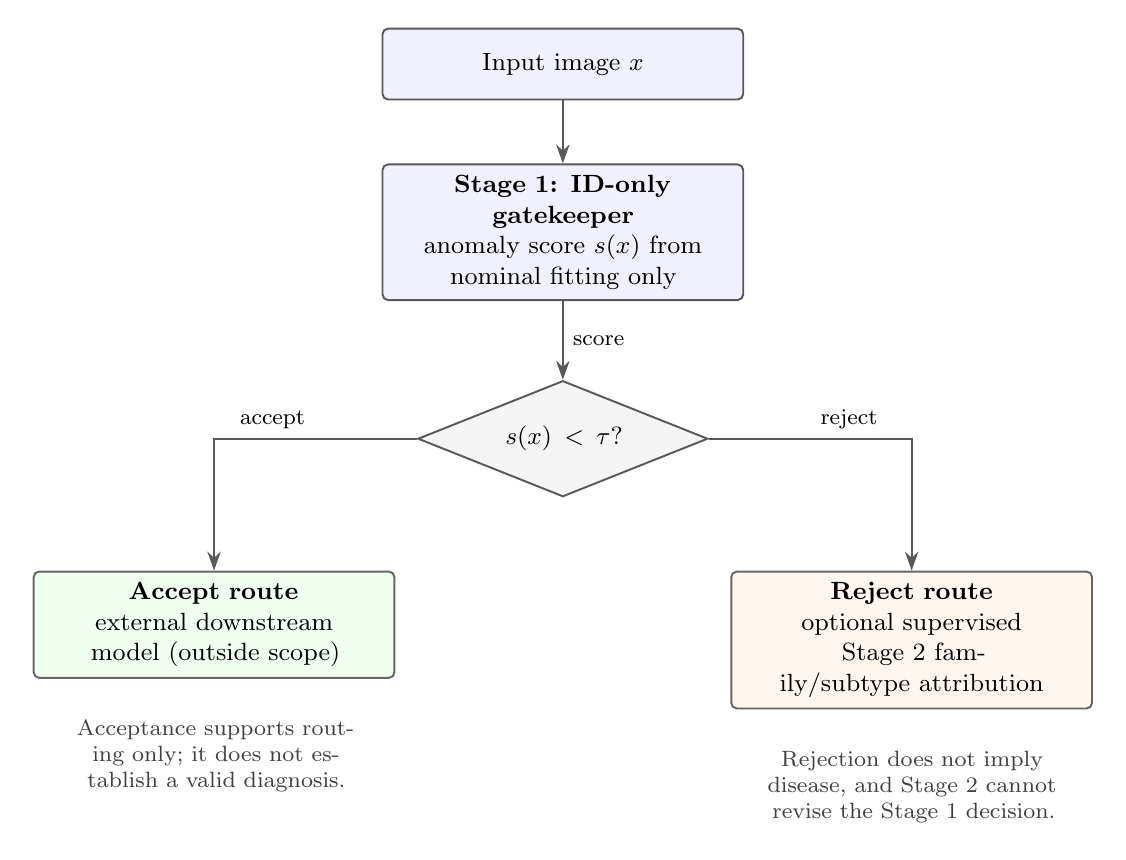
\begin{tikzpicture}[
        node distance=8mm and 13mm,
        every node/.style={font=\small},
        block/.style={
            rectangle,
            rounded corners=2pt,
            draw=black!65,
            line width=0.7pt,
            fill=blue!6,
            minimum height=9mm,
            text width=43mm,
            align=center,
            inner sep=4pt
        },
        decision/.style={
            diamond,
            aspect=2.5,
            draw=black!65,
            line width=0.7pt,
            fill=gray!8,
            text width=24mm,
            align=center,
            inner sep=2pt
        },
        endpoint/.style={
            rectangle,
            rounded corners=2pt,
            draw=black!60,
            line width=0.7pt,
            fill=green!6,
            minimum height=11mm,
            text width=43mm,
            align=center,
            inner sep=4pt
        },
        explain/.style={endpoint,fill=orange!7},
        flow/.style={-{Stealth[length=2.4mm,width=1.7mm]},line width=0.8pt,draw=black!65},
        note/.style={font=\footnotesize,text width=45mm,align=center,text=black!75}
    ]
        \node[block] (input) {Input image $x$};
        \node[block, below=of input] (gate) {\textbf{Stage 1: ID-only}\\
            \textbf{gatekeeper}\\anomaly score $s(x)$ from nominal fitting only};
        \node[decision, below=10mm of gate] (decision) {$s(x) < \tau$?};
        \node[endpoint, below left=13mm and 12mm of decision] (accept)
            {\textbf{Accept route}\\external downstream\\model (outside scope)};
        \node[explain, below right=13mm and 12mm of decision] (reject)
            {\textbf{Reject route}\\optional supervised\\Stage 2 family/subtype attribution};
        \node[note, below=4mm of accept] (acceptnote)
            {Acceptance supports routing only; it does not establish a valid diagnosis.};
        \node[note, below=4mm of reject] (rejectnote)
            {Rejection does not imply disease, and Stage 2 cannot revise the Stage 1 decision.};

        \draw[flow] (input) -- (gate);
        \draw[flow] (gate) -- node[right,font=\footnotesize] {score} (decision);
        \draw[flow] (decision) -| node[pos=0.25,above left,font=\footnotesize] {accept} (accept);
        \draw[flow] (decision) -| node[pos=0.25,above right,font=\footnotesize] {reject} (reject);
    \end{tikzpicture}
    \caption[Stage 1 gatekeeping and post-rejection explanation.]{
    \textbf{Gatekeeping and explanation boundary.} Stage~1 is fitted using
    nominal ID images only and makes the thresholded input-validity decision.
    Accepted images may proceed to an external downstream model, whereas only
    rejected images are eligible for optional supervised Stage~2 attribution.
    Neither branch is a diagnostic conclusion, and Stage~2 cannot alter the
    Stage~1 score or decision.}
    \label{fig:ood_pipeline}
\end{figure}


Figure~\ref{fig:ood_pipeline} fixes the interpretation used throughout: acceptance supports downstream routing, rejection indicates insufficient nominal support, and neither is a clinical diagnosis. Stage~2 supplies only an operational reason for rejection.

The following chapters review the literature, define the architecture and dataset, describe the methods and protocol, report the results, discuss their implications and limitations, document reproducibility, and conclude the study.

Figure~\ref{fig:dissertation_roadmap} summarises the structure and logical progression of the dissertation.

\begin{figure}[H]
\centering
\resizebox{0.82\textwidth}{!}{%
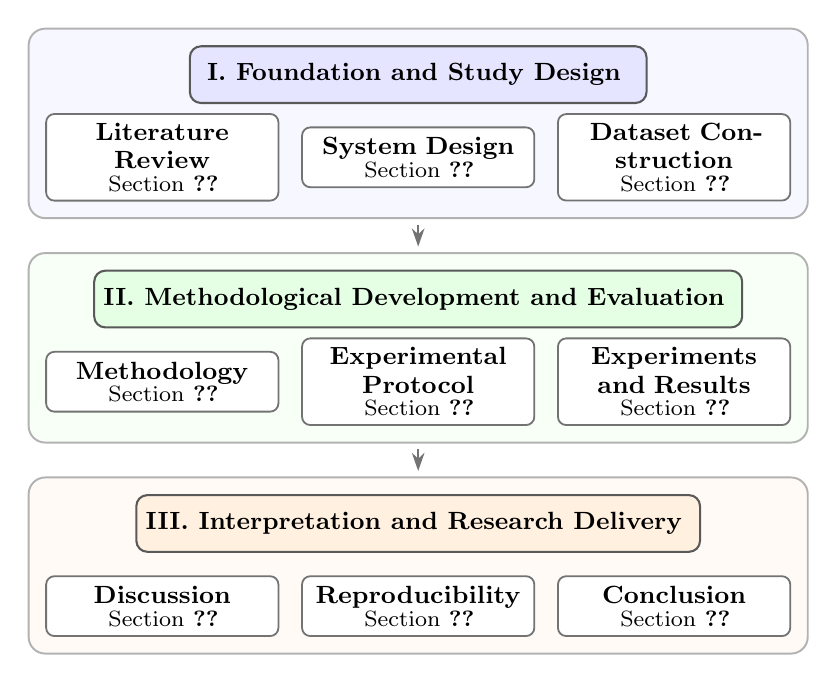
\begin{tikzpicture}[
    every node/.style={
        font=\fontsize{8.7pt}{10.2pt}\selectfont
    },
    phaseheader/.style={
        rectangle,
        rounded corners=4pt,
        minimum width=5.8cm,
        minimum height=0.72cm,
        align=center,
        draw=black!65,
        line width=0.75pt
    },
    chapter/.style={
        rectangle,
        rounded corners=3pt,
        minimum width=2.95cm,
        minimum height=0.76cm,
        text width=2.70cm,
        align=center,
        draw=black!55,
        line width=0.65pt,
        fill=white
    },
    phasegroup/.style={
        rectangle,
        rounded corners=6pt,
        draw=black!30,
        line width=0.7pt,
        inner sep=6pt
    },
    flowarrow/.style={
        -{Stealth[length=2.3mm,width=1.6mm]},
        line width=0.8pt,
        draw=black!55,
        shorten <=2pt,
        shorten >=2pt
    }
]

% ==========================================================
% Phase I
% ==========================================================
\node[
    phaseheader,
    fill=blue!10
] (phase1title) at (0,0) {
    \textbf{I. Foundation and Study Design}
};

\node[chapter] (lit) at (-3.25,-1.05) {
    \textbf{Literature Review}\\[-2pt]
    {\footnotesize Section~\ref{sec:literature_review}}
};

\node[chapter] (design) at (0,-1.05) {
    \textbf{System Design}\\[-2pt]
    {\footnotesize Section~\ref{sec:system_design}}
};

\node[chapter] (dataset) at (3.25,-1.05) {
    \textbf{Dataset Construction}\\[-2pt]
    {\footnotesize Section~\ref{sec:dataset}}
};

% ==========================================================
% Phase II
% ==========================================================
\node[
    phaseheader,
    fill=green!10
] (phase2title) at (0,-2.85) {
    \textbf{II. Methodological Development and Evaluation}
};

\node[chapter] (method) at (-3.25,-3.90) {
    \textbf{Methodology}\\[-2pt]
    {\footnotesize Section~\ref{sec:methodology}}
};

\node[chapter] (protocol) at (0,-3.90) {
    \textbf{Experimental Protocol}\\[-2pt]
    {\footnotesize Section~\ref{sec:experimental_protocol}}
};

\node[chapter] (results) at (3.25,-3.90) {
    \textbf{Experiments and Results}\\[-2pt]
    {\footnotesize Section~\ref{sec:results}}
};

% ==========================================================
% Phase III
% ==========================================================
\node[
    phaseheader,
    fill=orange!12
] (phase3title) at (0,-5.70) {
    \textbf{III. Interpretation and Research Delivery}
};

\node[chapter] (discussion) at (-3.25,-6.75) {
    \textbf{Discussion}\\[-2pt]
    {\footnotesize Section~\ref{sec:discussion}}
};

\node[chapter] (repro) at (0,-6.75) {
    \textbf{Reproducibility}\\[-2pt]
    {\footnotesize Section~\ref{sec:reproducibility}}
};

\node[chapter] (conclusion) at (3.25,-6.75) {
    \textbf{Conclusion}\\[-2pt]
    {\footnotesize Section~\ref{sec:conclusion}}
};

% ==========================================================
% Phase background cards
% ==========================================================
\begin{scope}[on background layer]

\node[
    phasegroup,
    fill=blue!3,
    fit=(phase1title)(lit)(design)(dataset)
] (phase1group) {};

\node[
    phasegroup,
    fill=green!3,
    fit=(phase2title)(method)(protocol)(results)
] (phase2group) {};

\node[
    phasegroup,
    fill=orange!4,
    fit=(phase3title)(discussion)(repro)(conclusion)
] (phase3group) {};

\end{scope}

% ==========================================================
% Short vertical arrows between phase cards
% ==========================================================
\draw[flowarrow]
    (phase1group.south)
    --
    (phase2group.north);

\draw[flowarrow]
    (phase2group.south)
    --
    (phase3group.north);

\end{tikzpicture}%
}
\caption[Dissertation chapter roadmap.]{\textbf{Dissertation roadmap.}
The dissertation progresses from foundation and study design to methodological evaluation, interpretation, and research delivery.}
\label{fig:dissertation_roadmap}
\end{figure}

\newpage
\section{Literature Review and Background}
\label{sec:literature_review}

\subsection{Problem Definition and Input-Anomaly Taxonomy}
\label{sec:problem}

The purpose of an upstream retinal-image gatekeeper is to determine whether an input is appropriate for a downstream analysis pipeline before any disease-specific prediction is attempted. This task differs from diagnostic classification. A diagnostic model discriminates among known clinical labels, whereas an input-validity model asks whether the image is sufficiently supported by the intended acquisition and modality distribution. Because the range of possible deployment errors is open-ended, the problem is naturally related to unsupervised anomaly detection and one-class learning, in which the nominal distribution is modelled without requiring an exhaustive catalogue of anomalous inputs \cite{ruff2021unifying,hong2024medicalood,heer2021oodblindspot}. In the present dissertation, Stage~1 is therefore fitted using in-distribution (ID) FAF-like images only and produces a continuous anomaly score for each query image.

\subsubsection{Mathematical Formulation and the Manifold Assumption}

Let
\begin{equation}
    \mathcal{D}_{\mathrm{train}}=\{x_i\}_{i=1}^{N},
\end{equation}
where each $x_i\in\mathcal{X}\subseteq\mathbb{R}^{H\times W\times C}$ is a nominal FAF-like training image. In this study, Stage~1 is fitted using synthetic FAF-like images rather than real clinical FAF acquisitions. The training samples are assumed to be drawn from an ID distribution $\mathcal{P}_{\mathrm{in}}$ that occupies a structured, lower-dimensional region of the ambient image space. This assumption is commonly expressed through a manifold $\mathcal{M}\subset\mathcal{X}$ representing the regularities shared by nominal inputs.

The anomaly space $\mathcal{P}_{\mathrm{ood}}$ is not represented by a single coherent distribution. It may include wrong imaging modalities, local annotations, image degradation, export artefacts, scanner shifts, and unrelated natural content. Rather than attempting to model this unbounded collection directly, an OOD detector learns a scoring function
\begin{equation}
    S:\mathcal{X}\rightarrow\mathbb{R},
\end{equation}
where larger values indicate weaker support from the learned ID reference distribution. The gatekeeping rule is obtained by applying an operating threshold $\tau$:
\begin{equation}
    A(x)=
    \begin{cases}
        \textsc{Accept}, & S(x)<\tau,\\
        \textsc{Reject}, & S(x)\geq\tau.
    \end{cases}
    \label{eq:decision_rule}
\end{equation}
The threshold determines the trade-off between recovering OOD inputs and falsely rejecting valid FAF-like images. Acceptance indicates only that the input is sufficiently consistent with the intended FAF domain to proceed to downstream analysis; it does not imply the absence of retinal pathology and does not guarantee the correctness of a subsequent diagnosis. Conversely, rejection indicates inadequate support from the learned reference distribution rather than evidence of disease.

\subsubsection{A Spectrum of Distributional Shifts}

OOD inputs in retinal workflows are heterogeneous, and their detectability depends on how they depart from the intended FAF distribution. Medical-imaging studies distinguish acquisition and domain shifts, local corruptions, and previously unseen semantic content, while retinal OOD studies show that visually related near-OOD cases can be more difficult than clearly unrelated far-OOD examples \cite{hong2024medicalood,araujo2023fewshot,wang2023uios}. Accordingly, this dissertation organises invalid inputs into three operational families. \emph{Modality shifts} retain some retinal structure but originate from an imaging modality other than FAF; \emph{sensory artefacts} alter an otherwise plausible FAF-like input through corruption, annotation, or post-processing; and \emph{semantic outliers} contain content unrelated to retinal imaging. These categories structure the literature discussion and subsequent evaluation, while the implemented subtypes, data sources, and manifest definitions are detailed in Section~\ref{sec:dataset}.

These families are operational categories rather than mutually exclusive geometric sets. Their relative proximity to the nominal distribution depends on the feature representation, image preprocessing, and anomaly-scoring method. Figure~\ref{fig:manifold_concept} therefore provides a simplified conceptual view rather than an empirical projection of the dataset.

% -----------------------------------------------------------
% TikZ Diagram: Conceptual Manifold
% Original visual design retained; spacing and labels refined
% -----------------------------------------------------------
\begin{figure}[htbp]
\centering
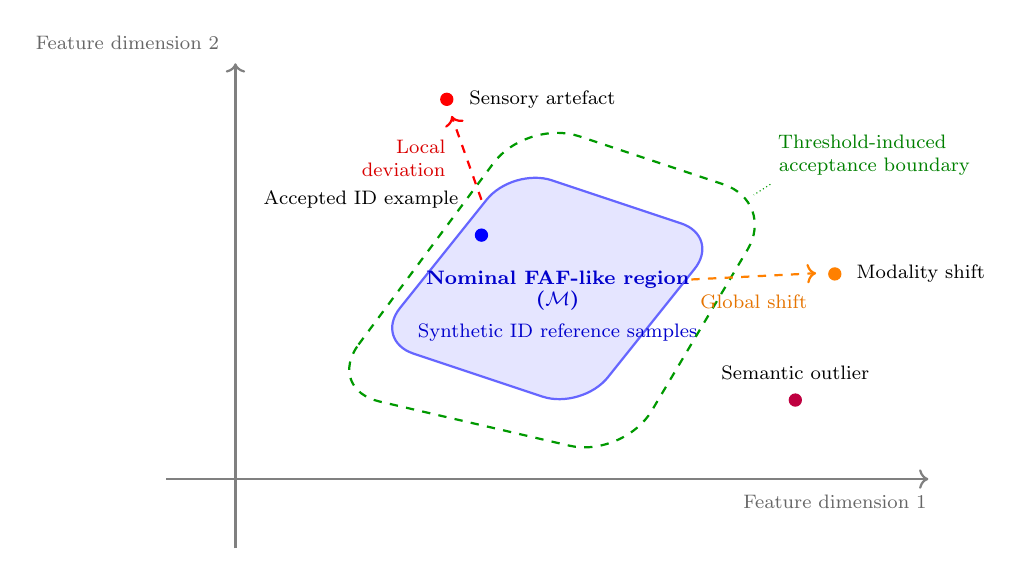
\begin{tikzpicture}[
    scale=0.88,
    transform shape,
    every node/.style={
        font=\fontsize{9.5pt}{11.5pt}\selectfont
    }
]

    % -------------------------------------------------------
    % Axes
    % -------------------------------------------------------
    \draw[thick, ->, gray]
        (-1,0) -- (10,0)
        node[
            anchor=north east,
            xshift=3pt,
            yshift=-3pt,
            text=gray!80!black,
            font=\footnotesize
        ] {Feature dimension 1};

    \draw[thick, ->, gray]
        (0,-1) -- (0,6)
        node[
            anchor=south east,
            xshift=-3pt,
            yshift=2pt,
            text=gray!80!black,
            font=\footnotesize
        ] {Feature dimension 2};

    % -------------------------------------------------------
    % Nominal FAF-like region
    % -------------------------------------------------------
    \draw[
        thick,
        fill=blue!10,
        draw=blue!60,
        rounded corners=15pt
    ]
        (2,2)
        -- (4,4.5)
        -- (7,3.5)
        -- (5,1)
        -- cycle;

    % Main label slightly reduced and repositioned
    \node[
        blue!80!black,
        font=\footnotesize\bfseries,
        align=center,
        text width=4.3cm
    ] at (4.65,2.72)
        {Nominal FAF-like region\\[-1pt]($\mathcal{M}$)};

    \node[
        blue!80!black,
        font=\footnotesize,
        align=center
    ] at (4.65,2.12)
        {Synthetic ID reference samples};

    % -------------------------------------------------------
    % Threshold-induced acceptance boundary
    % -------------------------------------------------------
    \draw[
        thick,
        dashed,
        draw=green!60!black,
        rounded corners=20pt
    ]
        (1.3,1.3)
        -- (4.2,5.2)
        -- (7.8,4.0)
        -- (5.6,0.3)
        -- cycle;

    \node[
        green!50!black,
        font=\footnotesize,
        align=left,
        anchor=west,
        text width=3.1cm
    ] (thresholdlabel) at (7.72,4.67)
        {Threshold-induced\\acceptance boundary};

    \draw[
        green!60!black,
        thin,
        densely dotted
    ]
        (thresholdlabel.south west)
        -- (7.48,4.10);

    % -------------------------------------------------------
    % Accepted ID example
    % -------------------------------------------------------
    \filldraw[blue]
        (3.55,3.52) circle (2.5pt);

    \node[
        anchor=south east,
        font=\footnotesize,
        text=black,
        align=right
    ] at (3.34,3.78)
        {Accepted ID example};

    % -------------------------------------------------------
    % Sensory artefact
    % -------------------------------------------------------
    \filldraw[red]
        (3.05,5.48) circle (2.5pt);

    \node[
        anchor=west,
        font=\footnotesize,
        text=black
    ] at (3.25,5.48)
        {Sensory artefact};

    \draw[
        ->,
        red,
        dashed,
        thick
    ]
        (3.55,4.03)
        -- (3.12,5.24)
        node[
            midway,
            left=5pt,
            font=\footnotesize,
            text=red!85!black,
            align=right
        ] {Local\\deviation};

    % -------------------------------------------------------
    % Modality shift
    % -------------------------------------------------------
    \filldraw[orange]
        (8.65,2.96) circle (2.5pt);

    \node[
        anchor=west,
        font=\footnotesize,
        text=black
    ] at (8.84,2.96)
        {Modality shift};

    % Label is attached directly to the arrow so that it
    % cannot fall to the origin or horizontal axis
    \draw[
        ->,
        orange,
        dashed,
        thick
    ]
        (6.58,2.88)
        -- (8.38,2.97)
        node[
            midway,
            below=4pt,
            font=\footnotesize,
            text=orange!90!black
        ] {Global shift};

    % -------------------------------------------------------
    % Semantic outlier
    % -------------------------------------------------------
    \filldraw[purple]
        (8.08,1.14) circle (2.5pt);

    \node[
        anchor=south,
        font=\footnotesize,
        text=black,
        yshift=5pt
    ] at (8.08,1.14)
        {Semantic outlier};

\end{tikzpicture}

\caption[Conceptual nominal support and OOD families.]{\textbf{Conceptual
feature-space view of FAF input validity.}
Nominal synthetic FAF-like inputs occupy a structured region, while modality shifts, sensory artefacts, and semantic outliers may deviate from it in different ways. The dashed contour is an illustrative acceptance boundary induced by the anomaly score and threshold, rather than an empirical embedding of the dataset.}
\label{fig:manifold_concept}
\end{figure}


The three families place different demands on the learned representation and anomaly score.

\paragraph{Modality shifts.}
Modality-shifted inputs may retain recognisable retinal anatomy while differing from FAF in acquisition physics, intensity distribution, colour composition, texture, or image layout. Representations dominated by high-level retinal structure may therefore underestimate the shift. Conversely, representations that rely too strongly on low-level acquisition characteristics may reject valid FAF images obtained under previously unseen devices or protocols. This tension makes modality shift a particularly important near-OOD challenge.

\paragraph{Sensory artefacts.}
Sensory artefacts preserve much of the underlying FAF-like content but introduce local deviations through annotations, watermarks, blur, cropping, noise, compression, or composite layouts. Because the affected region may occupy only a small proportion of the image, its contribution can be diluted by global image statistics, pooled feature representations, or globally averaged reconstruction losses. This motivates the evaluation of patch-level representations alongside image-level methods.

\paragraph{Semantic outliers.}
Semantic outliers contain content outside retinal imaging and are generally expected to receive weaker support from a nominal FAF representation. However, discriminative neural networks may still assign high confidence to unfamiliar inputs when local textures or shapes activate features associated with known classes \cite{nguyen2015deep,hendrycks2017baseline}. Semantic outliers therefore provide a useful far-OOD stress test, but strong performance on these visually distinct cases does not demonstrate that more subtle modality shifts or local artefacts have been resolved.

Representative benchmark samples, subtype definitions, provenance, counts, and audit procedures are presented in Section~\ref{sec:dataset}.

Having defined the one-class problem and the operational taxonomy, the following section reviews alternative ways of representing nominality and measuring deviation from it.

\subsection{OOD Detection Methodologies: A Comparative Analysis}
\label{sec:methods}

Visual anomaly-detection methods differ primarily in what they treat as evidence of normality. Some rely on low-level image statistics, others on the ability to reconstruct a nominal image, and others on distances or densities in a pretrained feature space \cite{ruff2021unifying,yang2024generalized,hong2024medicalood}. The implemented Stage~1 comparison in this dissertation evaluates five method families: image-statistics scoring, autoencoder reconstruction error, global feature $k$-nearest neighbours ($k$-NN), Mahalanobis feature distance, and PatchCore memory banks. The wider literature also includes PaDiM, knowledge-distillation methods, normalizing flows, transformer and foundation-model backbones, and self-supervised synthetic-anomaly methods. These broader approaches are reviewed to position the implemented comparison within the field; they are not presented as experiments completed in this dissertation.

\subsubsection{Image-Statistics Baselines}

Simple descriptors such as channel moments, intensity histograms, entropy,
edge density, and frequency statistics provide a transparent low-complexity
reference. In this benchmark, their diagnostic value is to reveal whether
gross acquisition cues already separate the evaluated categories before richer
retinal structure is modelled. They are inexpensive and interpretable but have
limited spatial specificity, so a small annotation may have little influence
on a globally aggregated descriptor.

\subsubsection{Reconstruction-Based Detection}

Autoencoders (AEs) and Variational Autoencoders (VAEs) are among the most established one-class anomaly-detection baselines in medical imaging \cite{baur2021autoencoders}. An encoder $E_{\theta}$ maps an input $x$ to a latent representation, and a decoder $D_{\phi}$ reconstructs the image. A common anomaly score is the squared reconstruction error
\begin{equation}
    S_{\mathrm{rec}}(x)=\lVert x-D_{\phi}(E_{\theta}(x))\rVert_2^2.
    \label{eq:reconstruction_score}
\end{equation}
The underlying assumption is that a model trained only on nominal images will reconstruct ID inputs better than OOD inputs.

The assumption is not guaranteed. A sufficiently expressive network may approximate an identity mapping and reproduce anomalous content more accurately than intended, while a restrictive bottleneck may remove clinically relevant detail from both ID and OOD images \cite{zavrtanik2021reconstruction,heer2021oodblindspot}. Neural networks also exhibit spectral bias, tending to learn lower-frequency structure before finer high-frequency components \cite{rahaman2019spectral}. This behaviour can be useful in image denoising, but it complicates quality control: a locally confined watermark or annotation may be attenuated, partially reconstructed, or diluted by a loss dominated by the unaffected retinal region. The reliability of reconstruction scoring therefore depends on network capacity, bottleneck design, loss function, preprocessing, and anomaly type. In this dissertation, the autoencoder is retained as a reconstruction baseline rather than assumed to provide a complete safety solution.

\subsubsection{Feature-Space Distance and Density Modelling}

Pretrained visual encoders shift the anomaly definition from pixel reconstruction to deviation in a learned representation. Generic CNN backbones can provide reusable edge, texture, shape, and semantic features, although transfer from natural-image pretraining to FAF remains imperfect \cite{yosinski2014transferable}. The quality of the resulting OOD boundary consequently depends on the representation, pooling strategy, feature depth, normalisation, and coverage of the nominal reference set.

\paragraph{Global feature $k$-NN.}
A global $k$-NN detector stores pooled feature vectors from nominal images and scores a query according to its distance from nearby reference samples. In its simplest form,
\begin{equation}
    S_{k\mathrm{NN}}(x)=\frac{1}{k}\sum_{j\in\mathcal{N}_k(\phi(x))}
    \lVert \phi(x)-\phi(x_j)\rVert_2,
\end{equation}
where $\phi(x)$ is a pooled embedding and $\mathcal{N}_k$ denotes the $k$ nearest nominal neighbours. The method is non-parametric and does not require the ID distribution to be Gaussian, but it depends on feature scaling, local density, the choice of $k$, and the coverage of the reference bank \cite{araujo2023fewshot,ahmadian2024novelty}. Global pooling can capture modality and semantic shifts effectively, yet may weaken sensitivity to small local artefacts.

\paragraph{Mahalanobis feature distance.}
Mahalanobis scoring estimates the nominal feature mean $\mu$ and covariance $\Sigma$ and measures deviation after accounting for feature correlations:
\begin{equation}
    S_{\mathrm{Mah}}(x)=
    \sqrt{\left(\phi(x)-\mu\right)^{T}
    \left(\Sigma+\lambda I\right)^{-1}
    \left(\phi(x)-\mu\right)},
    \label{eq:mahalanobis_score}
\end{equation}
where $\lambda I$ regularises the covariance estimate. Unlike unscaled Euclidean distance, Mahalanobis distance down-weights directions with high nominal variation and emphasises deviations along comparatively stable directions \cite{lee2018mahalanobis}. The model is compact and computationally efficient, but its interpretation relies on a sufficiently stable covariance estimate and can degrade when the embedded ID distribution is strongly multimodal or non-Gaussian. The global formulation used in this dissertation should be distinguished from patch-wise Gaussian methods such as PaDiM.

\paragraph{PaDiM.}
PaDiM estimates a Gaussian distribution for the feature vector at each spatial location \cite{defard2021padim}. For patch location $(i,j)$, its Mahalanobis score can be written as
\begin{equation}
    M(x_{i,j})=
    \sqrt{\left(\phi(x_{i,j})-\mu_{i,j}\right)^T
    \Sigma_{i,j}^{-1}
    \left(\phi(x_{i,j})-\mu_{i,j}\right)}.
\end{equation}
This spatially resolved formulation can support localisation, but location-specific statistics assume reasonably consistent alignment. Natural translation, rotation, cropping, or field-of-view variation may place otherwise normal structures in unexpected spatial cells. PaDiM is therefore relevant as a bridge between global covariance modelling and patch-level anomaly detection, although it is not included in the implemented experimental matrix.

\paragraph{PatchCore.}
PatchCore constructs a non-parametric memory bank of nominal patch embeddings and compares each test patch with its nearest stored feature \cite{roth2022towards}. Because the full memory bank may be large, a coreset $\mathcal{M}_C$ is selected to preserve representative coverage:
\begin{equation}
    \mathcal{M}_C^{*}=
    \arg\min_{\mathcal{M}_C\subset\mathcal{M}}
    \max_{m\in\mathcal{M}}
    \min_{c\in\mathcal{M}_C}
    \lVert m-c\rVert_2.
\end{equation}
A simplified image-level score is then obtained from the most anomalous query patch:
\begin{equation}
    S_{\mathrm{PC}}(x)=
    \max_{p\in\mathcal{P}(x)}
    \min_{c\in\mathcal{M}_C^{*}}
    \lVert p-c\rVert_2.
    \label{eq:patchcore_score}
\end{equation}
Patch-level comparison is attractive for local annotations and corruptions because a small discrepancy need not be averaged over the entire image. The patch distances can also be interpolated back to image space to provide localisation-oriented anomaly maps. However, the outcome depends on memory-bank coverage, feature normalisation, coreset construction, preprocessing, and feature depth. Shallow features retain detailed texture and acquisition signatures, deep features are more semantically invariant, and intermediate features often balance local sensitivity with structural abstraction \cite{yosinski2014transferable,zeiler2014visualizing}. This representation-depth trade-off motivates the L2, L3, L4, and L2+L3 PatchCore ablation evaluated later in the dissertation.

Figure~\ref{fig:architecture_comparison} contrasts the scoring mechanisms of an autoencoder and PatchCore. The comparison concerns scoring granularity rather than implying a universal performance ordering.

% -----------------------------------------------------------
% Comparative TikZ Diagram:
% Reconstruction versus Patch-Level Feature Matching
% -----------------------------------------------------------
\begin{figure}[htbp]
\centering
\resizebox{0.96\textwidth}{!}{%
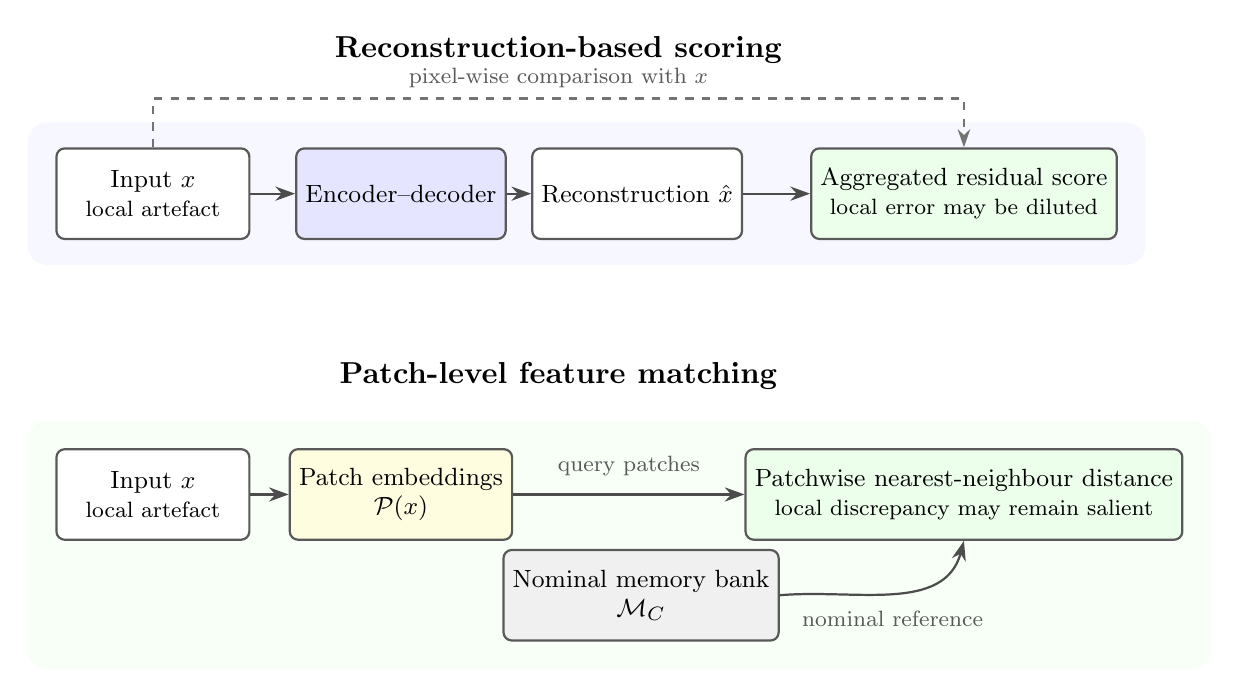
\begin{tikzpicture}[
    every node/.style={
        font=\fontsize{9.5pt}{11.5pt}\selectfont
    },
    block/.style={
        rectangle,
        rounded corners=3pt,
        draw=black!65,
        line width=0.8pt,
        minimum width=2.45cm,
        minimum height=1.15cm,
        align=center,
        fill=white
    },
    encoder/.style={
        block,
        fill=blue!10
    },
    feature/.style={
        block,
        minimum width=2.55cm,
        fill=yellow!12
    },
    memory/.style={
        block,
        minimum width=3.00cm,
        fill=gray!12
    },
    score/.style={
        block,
        minimum width=3.75cm,
        fill=green!8
    },
    arrow/.style={
        -{Stealth[length=2.5mm,width=1.8mm]},
        thick,
        draw=black!70
    },
    comparison/.style={
        -{Stealth[length=2.3mm,width=1.6mm]},
        dashed,
        line width=0.8pt,
        draw=black!55
    },
    annotation/.style={
        font=\footnotesize,
        text=black!65,
        fill=white,
        inner sep=1.5pt
    },
    paneltitle/.style={
        font=\fontsize{11pt}{13pt}\selectfont\bfseries,
        text=black
    }
]

% ===========================================================
% TOP PANEL: Reconstruction-based scoring
% ===========================================================

\node[paneltitle] at (5.15,1.82)
    {Reconstruction-based scoring};

\node[block] (aein) at (0,0)
    {Input $x$\\[-1pt]
     \footnotesize local artefact};

\node[encoder] (enc) at (3.15,0)
    {Encoder--decoder};

\node[block] (recon) at (6.15,0)
    {Reconstruction $\hat{x}$};

\node[score] (aesc) at (10.30,0)
    {Aggregated residual score\\[-1pt]
     \footnotesize local error may be diluted};

% Main reconstruction pathway
\draw[arrow] (aein) -- (enc);
\draw[arrow] (enc) -- (recon);
\draw[arrow] (recon) -- (aesc);

% Original input is compared with the reconstruction
\coordinate (compareleft) at ($(aein.north)+(0,0.62)$);
\coordinate (compareright) at ($(aesc.north)+(0,0.62)$);

\draw[comparison]
    (aein.north)
    -- (compareleft)
    -- node[
        midway,
        above=2pt,
        annotation
    ] {pixel-wise comparison with $x$}
    (compareright)
    -- (aesc.north);

% Upper-panel background
\begin{scope}[on background layer]
    \node[
        fill=blue!3,
        rounded corners=7pt,
        fit=(aein)(enc)(recon)(aesc),
        inner xsep=10pt,
        inner ysep=9pt
    ] {};
\end{scope}

% ===========================================================
% BOTTOM PANEL: Patch-level feature matching
% ===========================================================

\node[paneltitle] at (5.15,-2.32)
    {Patch-level feature matching};

\node[block] (pcin) at (0,-3.82)
    {Input $x$\\[-1pt]
     \footnotesize local artefact};

\node[feature] (patch) at (3.15,-3.82)
    {Patch embeddings\\[-1pt]
     $\mathcal{P}(x)$};

\node[score] (pcsc) at (10.30,-3.82)
    {Patchwise nearest-neighbour distance\\[-1pt]
     \footnotesize local discrepancy may remain salient};

\node[memory] (bank) at (6.20,-5.10)
    {Nominal memory bank\\[-1pt]
     $\mathcal{M}_{C}$};

% Query pathway
\draw[arrow] (pcin) -- (patch);

\draw[arrow]
    (patch.east)
    -- node[
        midway,
        above=3pt,
        font=\footnotesize,
        text=black!65
    ] {query patches}
    (pcsc.west);

% Fixed nominal reference pathway
\draw[arrow]
    (bank.east)
    to[out=5,in=-105]
    node[
        midway,
        below=3pt,
        font=\footnotesize,
        text=black!65
    ] {nominal reference}
    (pcsc.south);

% Lower-panel background
\begin{scope}[on background layer]
    \node[
        fill=green!3,
        rounded corners=7pt,
        fit=(pcin)(patch)(pcsc)(bank),
        inner xsep=10pt,
        inner ysep=10pt
    ] {};
\end{scope}

\end{tikzpicture}%
}

\caption[Reconstruction versus patch-level anomaly scoring.]{\textbf{Mechanistic
comparison of reconstruction and patch-level feature scoring.}
An autoencoder derives an aggregated residual by comparing the input with its reconstruction, which may dilute a spatially small artefact. PatchCore instead compares query patch embeddings with a fixed nominal memory bank, preserving local discrepancies in the anomaly score. The figure illustrates scoring granularity rather than a guaranteed performance ordering.}
\label{fig:architecture_comparison}
\end{figure}

\subsubsection{Broader Feature-Space and Representation-Learning Approaches}

\paragraph{Knowledge distillation.}
Student--teacher anomaly detectors train a student network to approximate a fixed teacher representation on nominal data \cite{salehi2021multiresolution}. At inference, disagreement between the teacher and student can be used as an anomaly score. A generic feature-matching objective is
\begin{equation}
    \mathcal{L}_{\mathrm{distill}}=
    \mathbb{E}_{x\sim\mathcal{P}_{\mathrm{in}}}
    \left[\lVert \widehat{T}(x)-\widehat{S}(x)\rVert_2^2\right].
\end{equation}
The approach avoids a growing nearest-neighbour bank and may support efficient inference, as illustrated by EfficientAD \cite{batzner2024efficientad}. Performance still depends on the teacher representation, student capacity, training stability, and whether disagreement generalises to unseen anomalies. It is not implemented here.

\paragraph{Normalizing flows.}
Normalizing flows learn an invertible mapping from a complex feature distribution to a tractable base density. The exact likelihood follows from the change-of-variables identity
\begin{equation}
    p_X(x)=p_Z(f(x))
    \left|\det\left(\frac{\partial f(x)}{\partial x}\right)\right|.
\end{equation}
FastFlow applies this principle to spatial feature maps \cite{yu2021fastflow}. Although flows provide explicit densities without a large memory bank, likelihood may reflect low-level statistics rather than semantic membership and can remain high for OOD samples. They are therefore relevant alternatives, not automatic clinical solutions.

\paragraph{Alternative backbones.}
CNNs impose locality and translation-related inductive biases through convolution, whereas Vision Transformers (ViTs) model long-range patch relationships through self-attention \cite{dosovitskiy2020image}. For queries $Q$, keys $K$, and values $V$, scaled dot-product attention is
\begin{equation}
    \begin{aligned}
        \mathbf{A}(Q,K)
        &=\operatorname{softmax}\left(\frac{QK^T}{\sqrt{d_k}}\right),\\
        \operatorname{Attention}(Q,K,V)
        &=\mathbf{A}(Q,K)V.
    \end{aligned}
\end{equation}
Neither architecture is uniformly superior for OOD detection: CNNs may preserve local texture, while transformers represent long-range structure differently. ViT-AD, DINOv2, and RETFound motivate future retinal representation studies \cite{mishra2021vt,oquab2023dinov2,zhou2023retfound}; the present comparison uses convolutional features.

% -----------------------------------------------------------
% Conceptual TikZ Diagram: CNN vs ViT
% -----------------------------------------------------------
\begin{figure}[htbp]
\centering
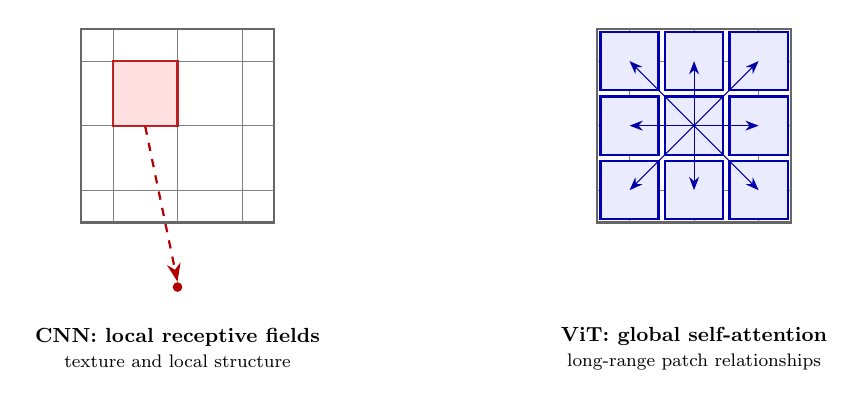
\begin{tikzpicture}[
    auto, scale=0.82, transform shape,
    every node/.style={font=\fontsize{9.5pt}{11.5pt}\selectfont},
    image_grid/.style={rectangle, draw=black!60, thick, minimum width=3cm, minimum height=3cm, align=center},
    kernel/.style={rectangle, draw=red!70!black, thick, fill=red!15, minimum width=1cm, minimum height=1cm, opacity=0.85},
    patch/.style={rectangle, draw=blue!70!black, thick, fill=blue!8, minimum width=0.9cm, minimum height=0.9cm},
    arrow/.style={thick, ->, >=Stealth, draw=black!70}
]

\node[image_grid] (cnn_img) at (0,0) {};
\draw[step=1cm, gray, very thin] (-1.5,-1.5) grid (1.5,1.5);
\node[kernel] (k1) at (-0.5,0.5) {};
\node[circle, fill=red!70!black, inner sep=1.5pt] (cnn_feat) at (0,-2.5) {};
\draw[arrow, red!70!black, dashed] (k1.south) -- (cnn_feat.north);
\node[align=center, font=\bfseries\small] at (0,-3.45)
    {CNN: local receptive fields\\\normalfont\footnotesize texture and local structure};

\node[image_grid] (vit_img) at (8,0) {};
\draw[step=1cm, gray, very thin] (6.5,-1.5) grid (9.5,1.5);
\node[patch] (p1) at (7,1) {}; \node[patch] (p2) at (8,1) {}; \node[patch] (p3) at (9,1) {};
\node[patch] (p4) at (7,0) {}; \node[patch] (p5) at (8,0) {}; \node[patch] (p6) at (9,0) {};
\node[patch] (p7) at (7,-1) {}; \node[patch] (p8) at (8,-1) {}; \node[patch] (p9) at (9,-1) {};
\foreach \j in {p1,p2,p3,p4,p6,p7,p8,p9} {
    \draw[arrow, blue!65!black, thin] (p5.center) -- (\j.center);
}
\node[align=center, font=\bfseries\small] at (8,-3.45)
    {ViT: global self-attention\\\normalfont\footnotesize long-range patch relationships};

\end{tikzpicture}
\caption[CNN and vision-transformer inductive biases.]{\textbf{Conceptual
inductive-bias comparison.} CNNs aggregate information through local
convolutions, whereas ViTs relate image patches through self-attention. These
architectural differences may alter sensitivity to local artefacts and global
structural shifts, but their suitability for FAF gatekeeping requires direct
empirical evaluation.}
\label{fig:cnn_vs_vit}
\end{figure}

\subsubsection{Proxy-Anomaly and Vision--Language Methods}

A further group of approaches uses nominal data to construct proxy anomalies or alternative supervisory signals. CutPaste inserts transformed image patches, Natural Synthetic Anomalies (NSA) applies more naturalistic blending, and DRAEM combines image reconstruction with a discriminative anomaly-segmentation network \cite{li2021cutpaste,schluter2022natural,zavrtanik2021draem}. Contrastive methods such as CSI apply distribution-shifting transformations to encourage nominal representations to separate from deliberately perturbed instances \cite{tack2020csi}. Related vision--language approaches, including WinCLIP, instead exploit CLIP-style representations and textual prompts to support zero-shot or few-shot anomaly classification and localisation \cite{jeong2023winclip}.

These methods can provide discriminative or spatial evidence without many labelled real anomalies, but may specialise to chosen corruptions, transformations, or prompts. They still require evaluation on heterogeneous unseen shifts. They are not implemented here: Stage~1 fitting remains ID-only, with OOD examples reserved for evaluation.

Taken together, the literature identifies complementary definitions of nominality rather than a universally superior detection strategy. Simple image-statistics baselines test whether broad shifts can already be identified from low-level appearance cues. Reconstruction methods assess whether an input can be reproduced through an ID-trained latent representation, while global feature methods measure its support within a pretrained embedding distribution. Patch-level approaches retain greater spatial sensitivity by comparing local representations with a nominal reference bank. Each paradigm introduces distinct assumptions and failure modes: low-level statistics provide limited semantic and spatial specificity; reconstruction errors may dilute small artefacts; global embeddings may overlook local deviations; and patch-based methods depend on feature depth and memory-bank coverage.

These trade-offs motivate the controlled Stage~1 comparison of image-statistics scoring, autoencoder reconstruction, global feature $k$-nearest-neighbour distance, Mahalanobis feature distance, and PatchCore layer variants conducted in this dissertation. Knowledge-distillation, normalizing-flow, transformer-based, foundation-model, proxy-anomaly, and vision--language approaches remain relevant alternatives in the wider literature, but fall outside the implemented experimental comparison.


\subsection{Open Problems and Research Gaps}
\label{sec:open_problems}

The transfer of one-class anomaly detection to retinal quality control remains constrained by distribution shift, threshold selection, interpretability, and the difference between controlled benchmarks and clinical deployment. Several analyses completed in this dissertation---including feature-layer ablation, subtype-level evaluation, robustness testing, threshold-policy comparison, and patch-level heatmaps---are motivated by these open issues. They reduce uncertainty within the current proof-of-concept benchmark but do not replace external validation on real clinical FAF data.

\subsubsection{Synthetic-to-Real Generalisation}

Synthetic data can improve reproducibility and reduce privacy and data-access barriers, but it may differ from clinical acquisitions in texture, noise, dynamic range, anatomical variability, preprocessing, and device-specific characteristics \cite{chen2021synthetic,veturi2023syntheye}. An anomaly detector trained only on synthetic FAF-like images may therefore learn generator- or pipeline-specific cues rather than the complete distribution of valid FAF. The risk is asymmetric: a narrow boundary may falsely reject valid real scans, whereas a permissive boundary may admit wrong modalities or corrupted inputs.

Figure~\ref{fig:sim_to_real} illustrates a possible synthetic-to-real mismatch schematically. The relative geometry is hypothetical and should not be interpreted as an empirical embedding of real clinical FAF data.

% -----------------------------------------------------------
% TikZ Diagram: Conceptual Sim-to-Real Gap
% Original visual design retained, with refined label placement
% -----------------------------------------------------------
\begin{figure}[htbp]
\centering
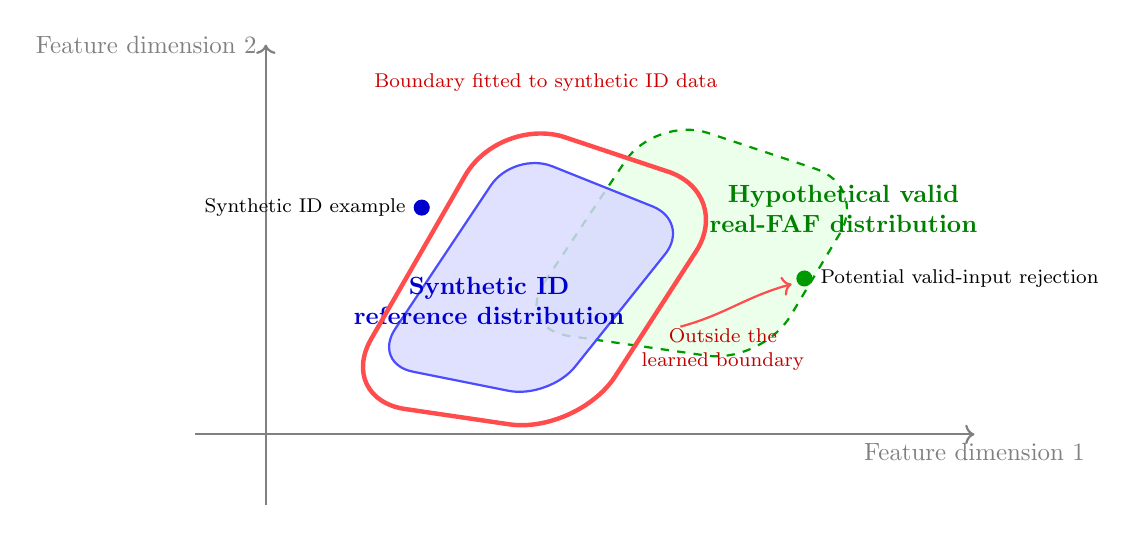
\begin{tikzpicture}[
    scale=0.9,
    transform shape,
    every node/.style={
        font=\fontsize{10pt}{12pt}\selectfont
    }
]

    % Axes
    \draw[thick, ->, gray]
        (-1,0) -- (10,0)
        node[anchor=north]
        {Feature dimension 1};

    \draw[thick, ->, gray]
        (0,-1) -- (0,5.5)
        node[anchor=east]
        {Feature dimension 2};

    % Hypothetical distribution of valid real clinical FAF
    \draw[
        thick,
        fill=green!10,
        fill opacity=0.78,
        draw=green!60!black,
        dashed,
        rounded corners=20pt
    ]
        (3.5,1.5)
        -- (5.5,4.5)
        -- (8.5,3.5)
        -- (7,1)
        -- cycle;

    \node[
        green!50!black,
        font=\bfseries,
        align=center
    ] at (8.15,3.18)
        {Hypothetical valid\\real-FAF distribution};

    % Synthetic ID reference distribution
    \draw[
        thick,
        fill=blue!15,
        fill opacity=0.82,
        draw=blue!70,
        rounded corners=15pt
    ]
        (1.5,1)
        -- (3.5,4)
        -- (6,3)
        -- (4,0.5)
        -- cycle;

    \node[
        blue!80!black,
        font=\bfseries,
        align=center
    ] at (3.15,1.88)
        {Synthetic ID\\reference distribution};

    % Boundary learned from synthetic ID data
    \draw[
        ultra thick,
        draw=red!70,
        rounded corners=25pt
    ]
        (1.0,0.5)
        -- (3.3,4.5)
        -- (6.6,3.4)
        -- (4.4,0.0)
        -- cycle;

    \node[
        red!80!black,
        font=\footnotesize,
        anchor=south
    ] at (3.95,4.72)
        {Boundary fitted to synthetic ID data};

    % Hypothetical valid real-FAF example outside the boundary
    \filldraw[green!60!black]
        (7.6,2.2) circle (3pt)
        node[
            anchor=west,
            font=\footnotesize,
            text=black,
            xshift=3pt
        ]
        {Potential valid-input rejection};

    \draw[
        ->,
        red!70,
        thick
    ]
        (5.85,1.52)
        to[out=15,in=195]
        (7.42,2.12);

    \node[
        red!75!black,
        font=\footnotesize,
        align=center
    ] at (6.45,1.2)
        {Outside the\\learned boundary};

    % Synthetic ID example
    \filldraw[blue!80!black]
        (2.2,3.2) circle (3pt)
        node[
            anchor=east,
            font=\footnotesize,
            text=black,
            xshift=-3pt
        ]
        {Synthetic ID example};

\end{tikzpicture}

\caption[Conceptual synthetic-to-real support mismatch.]{\textbf{Conceptual
synthetic-to-real mismatch in feature space.}
The blue region denotes the synthetic ID reference distribution used to fit the detector, and the red contour represents the acceptance boundary learned from synthetic ID data alone. The dashed green region illustrates a possible distribution of valid real clinical FAF acquisitions that is not fully covered by this synthetic-data boundary. Consequently, a valid real-FAF input may lie outside the learned boundary and be rejected. The relative positions and shapes are hypothetical and are not derived from an empirical embedding of real clinical FAF data in the present study.}
\label{fig:sim_to_real}
\end{figure}

The current project therefore uses held-out synthetic ID data as a fallback evaluation reference and reports proof-of-concept performance rather than clinical validity. Establishing external validity would require real FAF data collected across multiple devices, sites, acquisition protocols, and patient populations, together with a clinically justified distinction between acceptable acquisition variability and genuinely invalid inputs.

\subsubsection{Implications for Validation Design}

Standardised OOD benchmarks such as OpenOOD have improved comparability across detection settings \cite{yang2022openood,zhang2023openood}. Retinal quality control nevertheless requires additional structure: wrong modalities, sensory artefacts, semantic outliers, valid-ID false rejection, and threshold provenance should be reported separately rather than collapsed into one aggregate score. The corresponding fitting, calibration, and evaluation workflow is specified in Section~\ref{sec:experimental_protocol}.


\subsubsection{Representation Depth and Layer Selection}

Feature depth governs the balance between local detail and semantic invariance. Early CNN layers have small receptive fields and retain low-level texture, edge, and acquisition information \cite{zeiler2014visualizing}. This may help detect local overlays and noise, but it may also increase sensitivity to synthetic generation signatures or scanner-specific variation. Deeper layers aggregate wider context and produce more abstract representations \cite{yosinski2014transferable}. Such invariance can support semantic separation while attenuating subtle local corruptions. Intermediate representations can offer a compromise, but the optimum is task- and data-dependent rather than universal. This literature motivates the controlled PatchCore L2, L3, L4, and L2+L3 ablation conducted in the dissertation; the experiment tests the hypothesis rather than assuming that a particular layer is optimal.

\subsubsection{Evaluation Metrics and Threshold Provenance}

AUROC, AUPRC, and threshold-conditioned measures answer different questions. AUROC summarises how often an OOD example receives a higher score than an ID example over all thresholds. It is comparatively insensitive to the class ratio used to construct the evaluation set, but it does not directly express the precision or operational burden expected at a particular anomaly prevalence. AUPRC summarises precision--recall behaviour for the designated positive class and is often informative when attention centres on anomaly retrieval; however, it depends on the positive-class prevalence of the evaluation set \cite{saito2015precision}. In the present OOD-heavy benchmark, AUPRC must therefore be interpreted together with AUROC, family- and subtype-level performance, and threshold-conditioned ID rejection.

Let OOD denote the positive class. Precision and recall are
\begin{equation}
    \operatorname{Precision}=\frac{TP}{TP+FP},
    \qquad
    \operatorname{Recall}=\frac{TP}{TP+FN}.
\end{equation}
FPR at 95\% TPR provides a research operating point. If $\tau_{95}$ is selected as the smallest threshold achieving at least 95\% empirical OOD recall, then
\begin{equation}
    P_{x\sim\mathcal{P}_{\mathrm{ood}}}
    \left(S(x)\geq\tau_{95}\right)\geq 0.95,
\end{equation}
The corresponding ID false-rejection rate is then
\begin{equation}
    \operatorname{FPR@95\%TPR}=
    P_{x\sim\mathcal{P}_{\mathrm{in}}}
    \left(S(x)\geq\tau_{95}\right).
    \label{eq:fpr95}
\end{equation}
This quantity measures the proportion of ID inputs rejected while recovering at
least 95\% of the labelled OOD examples. It is useful for comparing detectors,
but a threshold selected with labelled OOD evaluation data should not be
described as a deployment threshold. Deployment-style policies must instead be
calibrated from held-out ID validation scores, for example through an ID
quantile or a fixed allowable ID rejection rate, and their provenance should
be reported explicitly. This distinction motivates the threshold-policy
analysis, bootstrap uncertainty, per-family and per-subtype reporting, and
explicit ID false-rejection analysis used later in the dissertation
\cite{yang2022openood,zhang2023openood}.

\subsubsection{Interpretability and Spatial Localisation}

A global anomaly score indicates that an input is insufficiently supported by
the nominal distribution, yet it provides no spatial origin for the score
\cite{choi2023concept}. PatchCore adds a spatial anomaly map: the nearest-memory
distance is retained at each query-patch location, arranged on the feature
grid, and interpolated to the input resolution. High-intensity regions mark
patches that depart most strongly from the nominal memory bank. The resulting
heatmap is localisation-oriented model evidence; it has not been validated as
a pixel-accurate segmentation or a clinical finding.

Spatial resolution remains limited by the feature-map stride and by interpolation back to the input image. Shallow features offer finer localisation but greater sensitivity to low-level variation; deeper features provide wider context but coarser maps. Gradient-based techniques such as Grad-CAM represent a related explanatory family \cite{selvaraju2017grad}, but they are conceptually distinct from the distance-based PatchCore maps implemented here and are not part of the present experiments. Future work may combine stronger ophthalmic representations, including RETFound-like features, with localisation-capable OOD methods, but any claimed improvement must be assessed under external clinical distribution shift rather than classification accuracy alone \cite{zhou2023retfound,oquab2023dinov2}.

\subsection{Post-Rejection Explanation and Stage~2 Attribution}
\label{sec:stage2_literature}

OOD detection, spatial localisation, and reason attribution answer different questions. Stage~1 asks whether an input is sufficiently supported by the nominal FAF distribution. A patch-level map indicates where feature-space discrepancy is concentrated. Stage~2 instead assigns a rejected input to one of the known operational reasons represented in the attribution taxonomy. Explainable OOD work similarly distinguishes the detection score from the concepts used to communicate why a sample appears OOD \cite{choi2023concept}.

Stage~2 is therefore designed as a supervised, closed-set task invoked only
after Stage~1 has rejected an input. OOD family and subtype labels are used to
train and evaluate this attribution module, but they are not used to fit the
Stage~1 gatekeeper. Conceptually, Stage~2 operates only on rejected inputs; its
standalone experimental evaluation is performed separately on the labelled
OOD set so that attribution performance can be isolated from Stage~1 threshold
errors. The label structure is hierarchical: the family level distinguishes
modality shift, sensory artefact, and semantic outlier, while the subtype level
provides a more specific operational reason. Hierarchical classification can
first estimate a coarse family and then restrict fine prediction to the
corresponding branch \cite{silla2011hierarchical}. This structure motivates
comparison between flat and hierarchical attribution models, although an
incorrect family decision can propagate to the subtype stage.

The explanation layer does not extend the open-world guarantee of the detector. It can name only reason categories represented during Stage~2 development, should not be applied to accepted inputs, and cannot compensate for an incorrect Stage~1 decision. Its output is a likely operational explanation rather than a clinical diagnosis. These boundaries preserve the primary contribution of the dissertation: an ID-only Stage~1 gatekeeper, supplemented---but not replaced---by a supervised post-rejection attribution module.

Together, these findings motivate the two-stage architecture, manifest-driven benchmark, ID-only fitting procedures, and safety-oriented evaluation framework developed in the following chapters.

\newpage
% Requires: graphicx, booktabs, tabularx, array

\section{System Requirements and Design}
\label{sec:system_design}

This section translates the research question into a system specification for
an upstream quality-control gatekeeper in retinal fundus autofluorescence
(FAF) imaging. The system assesses whether an incoming image is sufficiently
supported by a nominal FAF-like reference before it reaches any downstream
analysis model. Its purpose is input validation rather than disease
recognition. Detection, localisation, and post-rejection attribution are kept
as separate functions so that the primary Stage~1 decision remains ID-only.

\subsection{Design Objective and Operating Scope}
\label{subsec:design_objective}

Let $x\in\mathcal{X}$ denote an incoming image. Stage~1 assigns an anomaly
score $s(x)$, where larger values indicate weaker support from the nominal
reference. Given a threshold $\tau$, the gatekeeper applies

\begin{equation}
    d_{\tau}(x)=
    \begin{cases}
        \textsc{Accept}, & s(x)<\tau,\\
        \textsc{Reject}, & s(x)\geq\tau.
    \end{cases}
    \label{eq:system_gate_rule}
\end{equation}

An \textsc{Accept} decision means only that the image is sufficiently
consistent with the selected reference to continue through the wider
pipeline. It does not imply a healthy retina or guarantee a correct
downstream prediction. A \textsc{Reject} decision indicates insufficient
support under the learned reference rather than evidence of a specific
clinical condition.

The gatekeeper is intended to identify modality shifts, sensory artefacts, and
semantic outliers, as defined in Section~\ref{sec:dataset}. Errors originating
within a downstream diagnostic model, including class confusion, calibration
failure, and disease-specific bias, remain outside its scope. The present
study is also limited by its synthetic nominal data: Stage~1 fitting,
calibration, and fallback ID testing use synthetic FAF-like images rather than
a real clinical FAF cohort. The resulting system is therefore evaluated as a
benchmark-level proof of concept.

\subsection{Functional Requirements}
\label{subsec:functional_requirements}

Table~\ref{tab:system_requirements} summarises the system contract used
throughout the study.

\begin{table}[htbp]
    \centering
    \caption[FAF gatekeeper design requirements.]{Core design requirements of
    the FAF input gatekeeper.}
    \label{tab:system_requirements}

    \small
    \setlength{\tabcolsep}{5pt}
    \renewcommand{\arraystretch}{1.12}

    \begin{tabularx}{0.94\textwidth}{@{}
        >{\raggedright\arraybackslash}p{3.25cm}
        >{\raggedright\arraybackslash}X
    @{}}
        \toprule
        \textbf{Requirement} &
        \textbf{System implication} \\
        \midrule

        ID-only Stage~1 fitting &
        Stage~1 models and reference structures are constructed from nominal
        training data only; OOD labels are reserved for evaluation. \\

        Explicit score and threshold &
        Every successfully processed image receives an anomaly score and a
        documented thresholded decision. \\

        Threshold provenance &
        Thresholds derived from labelled OOD data are treated as retrospective
        research operating points, whereas operational prototype thresholds
        are calibrated from held-out ID validation scores. \\

        Explanation boundary &
        Localisation and Stage~2 attribution may accompany a rejection but
        cannot alter the Stage~1 score, threshold, or decision. \\

        Traceable failure handling &
        Configurations, scores, thresholds, and decisions remain traceable;
        decoding or processing failures are recorded separately from
        score-based rejection. \\

        \bottomrule
    \end{tabularx}
\end{table}

These requirements separate three operations that are often conflated:
constructing an anomaly score, comparing ID and OOD rankings, and selecting an
operating threshold. They also preserve the distinction between deciding that
an input is unsupported and explaining why it may have been rejected.

\subsection{Two-Stage System Architecture}
\label{subsec:two_stage_architecture}

The system contains two logically distinct stages. Stage~1 performs
input-validity detection from an ID-only nominal reference and controls
routing. Stage~2 is an optional supervised component invoked after rejection
to provide a likely technical explanation. Figure~\ref{fig:system_pipeline_overview}
shows the final architecture.

\begin{figure}[htbp]
    \centering
    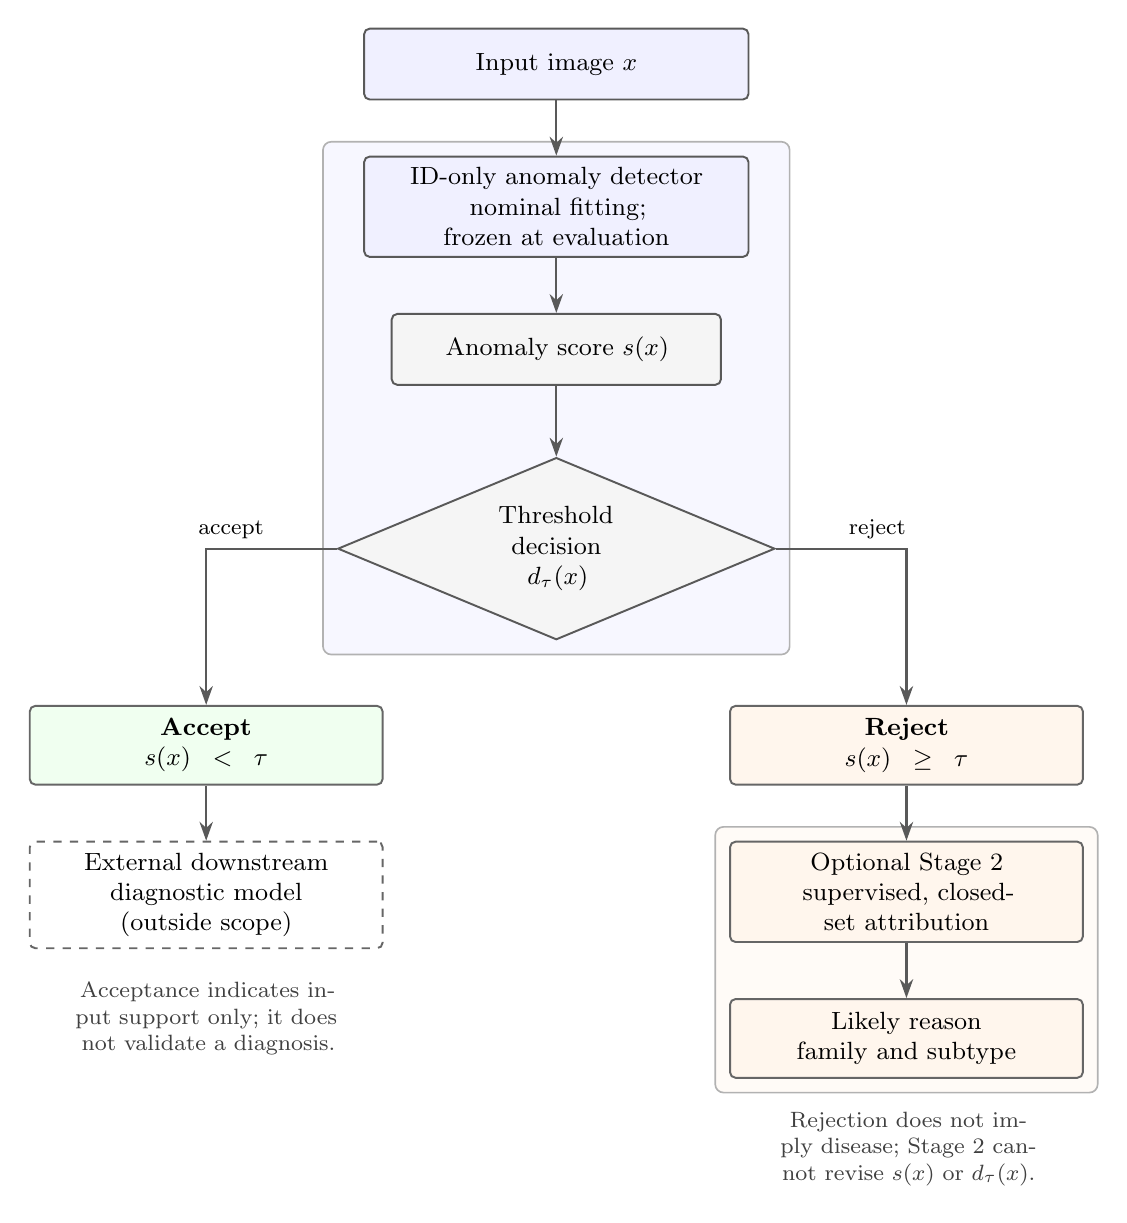
\begin{tikzpicture}[
        node distance=7mm and 16mm,
        every node/.style={font=\small},
        process/.style={
            rectangle,
            rounded corners=2pt,
            draw=black!65,
            line width=0.7pt,
            fill=blue!6,
            minimum height=9mm,
            text width=46mm,
            align=center,
            inner sep=4pt
        },
        score/.style={process,fill=gray!8,text width=39mm},
        decision/.style={
            diamond,
            aspect=2.4,
            draw=black!65,
            line width=0.7pt,
            fill=gray!8,
            text width=25mm,
            align=center,
            inner sep=2pt
        },
        route/.style={
            rectangle,
            rounded corners=2pt,
            draw=black!60,
            line width=0.7pt,
            fill=green!6,
            minimum height=10mm,
            text width=42mm,
            align=center,
            inner sep=4pt
        },
        rejectroute/.style={route,fill=orange!7},
        external/.style={route,dashed,fill=white},
        flow/.style={-{Stealth[length=2.4mm,width=1.7mm]},line width=0.8pt,draw=black!65},
        boundary/.style={font=\footnotesize,text=black!75,text width=43mm,align=center},
        group/.style={rounded corners=3pt,draw=black!30,line width=0.6pt,inner sep=5pt}
    ]
        \node[process] (input) {Input image $x$};
        \node[process, below=of input] (gate)
            {ID-only anomaly detector\\nominal fitting; frozen at evaluation};
        \node[score, below=of gate] (score) {Anomaly score $s(x)$};
        \node[decision, below=9mm of score] (decision)
            {Threshold decision\\$d_{\tau}(x)$};

        \node[route, below left=14mm and 8mm of decision] (accept)
            {\textbf{Accept}\\$s(x)<\tau$};
        \node[external, below=of accept] (downstream)
            {External downstream\\diagnostic model\\(outside scope)};
        \node[boundary, below=3mm of downstream] (acceptnote)
            {Acceptance indicates input support only; it does not validate a diagnosis.};

        \node[rejectroute, below right=14mm and 8mm of decision] (reject)
            {\textbf{Reject}\\$s(x)\geq\tau$};
        \node[rejectroute, below=of reject] (stage2)
            {Optional Stage 2\\supervised, closed-set attribution};
        \node[rejectroute, below=of stage2] (reason)
            {Likely reason\\family and subtype};
        \node[boundary, below=3mm of reason] (rejectnote)
            {Rejection does not imply disease; Stage 2 cannot revise $s(x)$ or $d_{\tau}(x)$.};

        \draw[flow] (input) -- (gate);
        \draw[flow] (gate) -- (score);
        \draw[flow] (score) -- (decision);
        \draw[flow] (decision) -| node[pos=0.24,above left,font=\footnotesize] {accept} (accept);
        \draw[flow] (decision) -| node[pos=0.24,above right,font=\footnotesize] {reject} (reject);
        \draw[flow] (accept) -- (downstream);
        \draw[flow] (reject) -- (stage2);
        \draw[flow] (stage2) -- (reason);

        \begin{scope}[on background layer]
            \node[group,fill=blue!3,fit=(gate)(score)(decision)] {};
            \node[group,fill=orange!3,fit=(stage2)(reason)] {};
        \end{scope}
    \end{tikzpicture}
    \caption[Canonical two-stage FAF input-control architecture.]{
    \textbf{Canonical two-stage architecture.} Stage~1 is fitted only on
    nominal ID images and owns the score, threshold, and routing decision.
    Accepted inputs may proceed to an external diagnostic model outside this
    work. Only rejected inputs may enter optional supervised, closed-set
    Stage~2 attribution, which cannot alter the Stage~1 score or decision.}
    \label{fig:system_pipeline_overview}
\end{figure}

A single supervised classifier could be trained to separate the implemented
ID and OOD categories, but such a system would optimise directly against the
known benchmark taxonomy. The two-stage design instead assigns different
responsibilities to the two forms of learning: Stage~1 estimates support under
the nominal distribution, while Stage~2 communicates a known reason for an
existing rejection.

\subsubsection{Stage~1: ID-Only Input-Validity Detection}
\label{subsubsec:stage1_design}

Stage~1 evaluates each input against parameters, statistics, or stored
features obtained from nominal training images:

\begin{equation}
    f_{1}\!\left(x;\Theta_{\mathrm{ID}}\right)
    \longrightarrow s(x)
    \longrightarrow d_{\tau}(x),
    \label{eq:stage1_system_interface}
\end{equation}

where $\Theta_{\mathrm{ID}}$ denotes the fitted nominal reference. The training
split constructs this reference, the held-out ID validation split supports
ID-calibrated threshold selection, and the synthetic ID fallback and labelled
OOD sets are used only for retrospective evaluation. OOD family and subtype
labels do not enter Stage~1 fitting. Method-specific implementations are
described in Section~\ref{sec:methodology}, while threshold policies are
defined in Section~\ref{sec:experimental_protocol}.

Patch-based configurations may additionally return a spatial anomaly map.
Such maps indicate where patch-level features deviate most strongly from the
nominal memory bank. They are treated as localisation-oriented model evidence,
not as pixel-accurate segmentation, causal explanation, or evidence of retinal
pathology.

\subsubsection{Stage~2: Optional Post-Rejection Attribution}
\label{subsubsec:stage2_design}

Stage~2 is invoked only after Stage~1 has returned \textsc{Reject}. Its output
is

\begin{equation}
    f_{2}(x)
    \longrightarrow
    \left(
        \widehat{y}_{\mathrm{family}},
        \widehat{y}_{\mathrm{subtype}}
    \right),
    \label{eq:stage2_system_interface}
\end{equation}

where the predictions describe a likely operational reason from the finite
attribution taxonomy. Stage~2 is supervised because its purpose is to name a
known rejection reason rather than to determine whether the image is nominal.
The implemented subtype model is hierarchical and uses the predicted family
for routing at inference, making it non-oracle.

Stage~2 cannot alter the anomaly score, threshold, or gate decision. Its label
space is closed-set, so an unseen failure mechanism may be assigned
imperfectly to an existing category. The output is therefore a likely
technical explanation rather than a clinical diagnosis or a complete causal
account.

\subsection{Decision Flow and Interface Boundaries}
\label{subsec:decision_flow}

The operational flow begins with image loading and method-specific
preprocessing. A successfully processed image receives a Stage~1 score and
thresholded decision. Accepted inputs may be forwarded to an external
downstream model; rejected inputs are blocked from that route and may
optionally receive localisation or Stage~2 attribution.

Unreadable, missing, or unsupported files are treated as processing failures,
not model-based OOD decisions. Both outcomes prevent downstream routing, but
only a successfully scored image receives an anomaly score. Recording these
states separately avoids attributing a learned decision to an input that was
never evaluated.

Detection, localisation, and attribution also have distinct evidential roles.
Detection controls routing, localisation indicates where feature discrepancy
is concentrated, and attribution selects the most plausible known reason for
rejection. Strong performance in one role does not establish performance in
another. The downstream diagnostic model remains an external consumer of
accepted inputs and is neither implemented nor evaluated in this dissertation.

\subsection{Safety, Interpretability, and Traceability Requirements}
\label{subsec:safety_traceability}

The safety-oriented objective is to reduce the chance that an unsupported
input is passed silently to a downstream model. This is not equivalent to a
claim of clinical safety. A restrictive threshold may improve OOD recall while
increasing false rejection of nominal inputs, whereas a permissive threshold
reduces false rejection at the cost of missed OOD cases. A thresholded result
must therefore be reported together with its selection policy, ID
false-rejection rate, and OOD recall. No operating point is assumed to be
universally optimal.

The system exposes three complementary forms of evidence: the continuous
anomaly score, optional PatchCore localisation maps, and optional Stage~2
reason labels. None has the status of clinical ground truth. Scores are
detector-relative, heatmaps do not establish pathology or causality, and
attribution labels describe operational categories rather than diagnoses.

Traceability requires each reported result to remain connected to its data
manifest, configuration, nominal reference, threshold policy, score file,
metric table, and figure. Dataset controls are described in
Section~\ref{sec:dataset}, and repository-level validation and evidence
indexing are described in Section~\ref{sec:reproducibility}.

\subsection{Computational Requirements and Explicit Non-Goals}
\label{subsec:computational_non_goals}

The implementation supports reproducible fitting, calibration, and scoring
rather than a predetermined real-time clinical latency target. Each Stage~1
method must be able to score an unseen image using a stored model or nominal
reference, with fitting, threshold calibration, and evaluation executed
separately. The evaluated methods have different storage and inference costs;
these are reported as local experimental measurements in
Section~\ref{sec:results}, not as hardware-independent deployment guarantees.

The system is not intended to diagnose retinal disease, certify clinical image
quality, replace expert review, detect every future anomaly, produce
pixel-accurate anomaly segmentation, or prescribe a universal threshold. It
also does not evaluate the effect of gatekeeping on any specific downstream
diagnostic model. Most importantly, the present study does not establish
external performance on real multi-centre clinical FAF data or support claims
of regulatory or hospital readiness.

Within these boundaries, the architecture provides a controlled framework for
testing whether nominal-only modelling can support FAF input rejection,
whether patch-level methods can provide useful spatial evidence, and whether
rejected inputs can be assigned plausible technical reasons without
introducing OOD supervision into Stage~1.

The next section describes the benchmark used to instantiate this design,
including the synthetic nominal reference, OOD taxonomy, manifest-defined
splits, image-integrity checks, and synthetic-to-real limitations.


\newpage

\section{Dataset Construction and Validation}
\label{sec:dataset}

This section describes the benchmark used to instantiate the system defined in
Section~\ref{sec:system_design}. The dataset supports three distinct
experimental roles: nominal-only fitting and calibration of the Stage~1
gatekeeper, controlled evaluation against structured OOD inputs, and
supervised Stage~2 reason attribution. These roles are represented through
separate version-controlled manifests so that labelled OOD examples remain
isolated from Stage~1 fitting.

The package contains 3,100 unique image files: 1,000 synthetic FAF-like ID
images and 2,100 OOD images. Several task-specific views are derived from this
fixed collection for fitting, calibration, balanced evaluation, and Stage~2
attribution. Their manifest row counts are therefore non-additive.

\subsection{Dataset Rationale and Scope}
\label{subsec:dataset_rationale}

The benchmark was constructed around the requirements of an upstream FAF
input gatekeeper. Stage~1 requires nominal examples from which to construct an
ID reference, but its fitting procedure must remain independent of any fixed
catalogue of anomalies. Evaluation instead requires heterogeneous inputs that
depart from the intended domain in controlled and interpretable ways.

The OOD collection therefore covers three operational families. Modality
shifts retain an ophthalmic context but originate from an unintended imaging
modality. Sensory artefacts preserve an underlying FAF-like image while
introducing an overlay, corruption, crop, or layout change. Semantic outliers
contain content unrelated to retinal imaging. This structure supports
family- and subtype-level analysis without implying that the taxonomy is
exhaustive.

The benchmark was designed for method comparison and stress testing rather
than prevalence estimation. Its class proportions do not represent the
frequency of invalid inputs in clinical practice. It also contains no disease
targets: the ID designation denotes membership in the synthetic FAF-like
reference distribution, not the absence of retinal pathology.

\subsection{Image Collection and Data Sources}
\label{subsec:dataset_sources}

The nominal collection contains 1,000 synthetic FAF-like images from the UCL
SynthEye synthetic FAF source \cite{uclSyntheyeDataset2025}, partitioned
deterministically into 700 training, 150 validation, and 150 held-out fallback
test images. The source metadata did not support clinically stratified
partitioning by disease, scanner, or patient subgroup, and the fallback test is
therefore not a real clinical FAF validation set.

The sensory-artefact collection contains 1,200 images derived from held-out
synthetic FAF-like parents. Eight transformations were applied, with 150
examples per subtype: text watermark, rectangle annotation, arrow annotation,
composite layout, blur, border crop, Gaussian noise, and JPEG compression.
Parent images used for these transformations were excluded from the Stage~1
training split. Each derived image retains a content hash and a parent-image
hash so that related variants can be audited.

The modality-shift collection contains 200 colour-fundus images and 200 OCT
screenshots imported from prepared public OOD source buckets. The
semantic-outlier collection contains 500 prepared natural images imported from
a prepared public semantic-outlier source bucket. The committed manifests
confirm the benchmark source buckets
(\texttt{prepared\_colour\_fundus},
\texttt{prepared\_oct\_screenshot}, and
\texttt{prepared\_cifar10\_or\_natural}), but they do not retain the original
upstream filenames, source URLs, or per-image licence records needed to assign
each imported image to a specific public dataset. Redistribution remains
subject to the terms of the original external sources.

\subsection{Manifest-Defined Experimental Views}
\label{subsec:manifest_representation}

Dataset membership is defined through version-controlled CSV manifests rather
than inferred dynamically from directory contents. Each row records the
relative image path, experimental role, ID/OOD label, split, OOD family and
subtype, source-bucket label, and available derivation metadata. Content hashes,
parent-image hashes, transformation details, and audit notes are retained
where applicable.

This design separates physical storage from experimental use. A single image
may be referenced by the full OOD collection, a balanced evaluation view, and
a Stage~2 split without being duplicated on disk. It also makes the role of
every image explicit and prevents unnoticed directory changes from altering
an experiment.

Table~\ref{tab:dataset_splits} uses five concise status labels. A
\emph{primary split} partitions the nominal image collection; a
\emph{primary collection} contains imported standalone images; and
\emph{derived images} are generated from recorded parents. A
\emph{manifest view} reuses existing files for evaluation, while a
\emph{grouped split} partitions those files by parent hash or image path.
Manifest views and grouped splits create no additional images, so their row
counts are not added to the unique-file total.

For Stage~1, binary and taxonomic labels are consulted only after anomaly
scores have been generated. They support evaluation and stratified reporting
but do not contribute to detector fitting or nominal reference construction.
Stage~2 uses separate OOD-only manifests because family and subtype labels are
supervised attribution targets.

\subsection{Stage~1 and Stage~2 Data Splits}
\label{subsec:dataset_splits}

Table~\ref{tab:dataset_splits} summarises the principal manifest-defined
views. Stage~1 fitting uses only the 700-image ID training set. A separate
150-image ID validation set supports ID-calibrated threshold selection, and a
further 150 synthetic FAF-like images provide the held-out ID fallback test
set. OOD examples are introduced only during evaluation.

Stage~2 uses a separate parent-grouped 60/20/20 partition with seed 42.
Parent grouping means that all rows sharing the same normalised parent
identifier are assigned together to exactly one of the training, validation,
or test partitions. The identifier is the non-empty
\texttt{parent\_image\_\allowbreak hash} when available and otherwise the exact
image path. Thus, all eight sensory-artefact variants derived from one
synthetic parent remain in one partition, while standalone modality-shift and
semantic-outlier images form singleton groups. The resulting manifests contain
1,260, 420, and 420 rows, respectively.

\begin{table}[p]
    \centering
    \caption[Dataset collections and experimental views.]{Dataset collections,
    manifest-defined views, and experimental roles.}
    \label{tab:dataset_splits}

    \small
    \setlength{\tabcolsep}{1.95pt}
    \setlength{\extrarowheight}{1.0pt}
    \renewcommand{\arraystretch}{1.08}

    \sisetup{
        group-separator = {,},
        group-minimum-digits = 4,
        table-number-alignment = right
    }

    \begin{tabularx}{0.99\textwidth}{@{}
        >{\raggedright\arraybackslash}p{2.15cm}
        >{\centering\arraybackslash}p{0.78cm}
        >{\raggedright\arraybackslash}p{1.58cm}
        >{\raggedright\arraybackslash}p{2.15cm}
        >{\raggedright\arraybackslash}X
        >{\raggedright\arraybackslash}p{1.48cm}
        S[table-format=4.0]
    @{}}
        \toprule
        \makecell[l]{\textbf{Dataset /}\\\textbf{split}} &
        \textbf{Use} &
        \makecell[l]{\textbf{Data}\\\textbf{status}} &
        \makecell[l]{\textbf{Source /}\\\textbf{grouping}} &
        \textbf{Role} &
        \textbf{Targets} &
        {\textbf{Images}} \\
        \midrule

        \rowcolor{black!7}
        \multicolumn{7}{@{}l}{\textit{Physical image collections and nominal splits}}\\
        \addlinespace[0.12em]

        ID training & S1 & Primary split & UCL SynthEye FAF &
        Fit nominal reference & ID & 700 \\
        ID validation & S1 & Primary split & UCL SynthEye FAF &
        Calibrate ID threshold & ID & 150 \\
        ID fallback test & S1 & Primary split & UCL SynthEye FAF &
        Estimate ID false rejection & ID & 150 \\
        Imported OOD & Both & Primary collection & Public-source buckets &
        Modality and semantic OOD source & \makecell[l]{Family /\\subtype} & 900 \\
        Sensory artefacts & Both & Derived images & Held-out SynthEye parents &
        Artefact OOD source & \makecell[l]{Family /\\subtype} & 1200 \\

        \addlinespace[0.20em]
        \midrule
        \addlinespace[0.10em]
        \rowcolor{black!7}
        \multicolumn{7}{@{}l}{\textit{Manifest-defined Stage~1 evaluation views}}\\
        \addlinespace[0.12em]

        Full OOD & Both & Manifest view & All OOD files &
        Complete evaluation; Stage~2 source & \makecell[l]{Family /\\subtype} & 2100 \\
        Family-balanced OOD & S1 & Manifest view & Full OOD collection &
        Family-level analysis & \makecell[l]{Eval.\\only} & 1200 \\
        Subtype-balanced OOD & S1 & Manifest view & Full OOD collection &
        Primary Stage~1 comparison & \makecell[l]{Eval.\\only} & 1650 \\

        \addlinespace[0.20em]
        \midrule
        \addlinespace[0.10em]
        \rowcolor{black!7}
        \multicolumn{7}{@{}l}{\textit{Parent-grouped Stage~2 partitions}}\\
        \addlinespace[0.12em]

        Attribution training & S2 & Grouped split & Parent/path groups &
        Fit attribution models & \makecell[l]{Family /\\subtype} & 1260 \\
        Attribution validation & S2 & Grouped split & Parent-disjoint &
        Select attribution models & \makecell[l]{Family /\\subtype} & 420 \\
        Attribution test & S2 & Grouped split & Parent-disjoint &
        Final attribution evaluation & \makecell[l]{Family /\\subtype} & 420 \\

        \bottomrule
    \end{tabularx}

    \vspace{0.35em}
    \begin{minipage}{\textwidth}
        \footnotesize
        \setlength{\parindent}{0pt}
        \emph{Note.}
        S1 and S2 denote Stage~1 and Stage~2; Both indicates use in both stages. The 1,000 ID images, 900 imported
        OOD images, and 1,200 derived sensory artefacts constitute 3,100 unique
        files. Manifest views reuse these files. The Stage~2 partitions divide
        the same 2,100 OOD files into 1,260 training, 420 validation, and 420
        test examples.
    \end{minipage}
\end{table}

Imported OOD images remain traceable to their prepared source buckets. The
final manifests do not retain immutable upstream filenames or per-image source
URLs.

The subtype-balanced OOD set is used for the primary Stage~1 comparison
because it gives equal weight to each of the 11 implemented subtypes. The full
OOD collection contains 1,200 sensory artefacts, 400 modality shifts, and 500
semantic outliers, so an unbalanced aggregate would give greater influence to
the largest family.

Subtype balancing does not make the benchmark prevalence neutral. The primary
comparison still contains 1,650 OOD and 150 ID images and is therefore
OOD-heavy. This composition is particularly relevant to AUPRC, which depends
on positive-class prevalence. Metric definitions and threshold policies are
specified in Section~\ref{sec:experimental_protocol}.

\subsection{OOD Family and Subtype Taxonomy}
\label{subsec:dataset_taxonomy}

The benchmark contains three OOD families and 11 subtypes.
Table~\ref{tab:ood_taxonomy} presents the complete taxonomy and the image
counts in the full OOD collection.

\begin{table}[htbp]
    \centering
    \caption[OOD taxonomy and image counts.]{OOD taxonomy and image counts in
    the full evaluation set.}
    \label{tab:ood_taxonomy}

    \small
    \setlength{\tabcolsep}{6pt}
    \renewcommand{\arraystretch}{1.18}

    \sisetup{
        group-separator = {,},
        group-minimum-digits = 4,
        table-number-alignment = center
    }

    \begin{tabularx}{0.94\textwidth}{@{}
        >{\raggedright\arraybackslash}p{3.05cm}
        >{\raggedright\arraybackslash}X
        S[table-format=4.0]
    @{}}
        \toprule
        \textbf{OOD family} &
        \textbf{Implemented subtypes} &
        \multicolumn{1}{c}{\textbf{Images}} \\
        \midrule

        Modality shift &
        Colour fundus; OCT screenshot &
        400 \\

        \addlinespace[0.35em]

        Sensory artefact &
        Text watermark; rectangle annotation; arrow annotation; composite
        layout;\newline
        blur; border crop; Gaussian noise; JPEG compression &
        1200 \\

        \addlinespace[0.35em]

        Semantic outlier &
        Natural-image content &
        500 \\

        \bottomrule
    \end{tabularx}
\end{table}

Modality shifts test whether the detector distinguishes FAF from other retinal
modalities rather than merely recognising retinal anatomy. Sensory artefacts
test both local and diffuse changes while preserving the overall FAF-like
content. Semantic outliers test broad separation from non-retinal content.
These categories are operational rather than clinical and describe how an
input departs from the intended image domain.

Figure~\ref{fig:anomaly_examples} shows representative examples. The panels
are illustrative and do not encode category prevalence, detection difficulty,
or clinical ground truth.

\begin{figure}[p]
    \centering
    \includegraphics[width=\textwidth]{%
        reports/dissertation_figures/figure_dataset_taxonomy_12_panel_vincent_round3.pdf}
    \caption[One nominal example and all 11 OOD subtypes.]{
    \textbf{Benchmark taxonomy examples.} Panel (a) shows one synthetic
    FAF-like ID sample. Panels (b)--(d) show the colour-fundus, OCT-screenshot,
    and natural-image OOD subtypes. Panels (e)--(l) show all eight sensory
    artefacts generated from held-out synthetic FAF-like parents. Panels
    (i)--(l) use the same clearer, higher-contrast synthetic FAF-like base
    image so that the four artefacts remain visible at page scale. The inset in
    panel (g) magnifies the original watermark region. The modality-shift and
    semantic panels come from prepared public-source collections recorded at
    source-bucket level. The montage illustrates the taxonomy only and does not
    represent prevalence, detection difficulty, or clinical validity.}
    \label{fig:anomaly_examples}
\end{figure}

\subsection{Integrity, Provenance, and Split Dependence}
\label{subsec:dataset_validation}

All 3,100 packaged files were present and opened successfully during the
automated audit; no corrupt, missing, or blank images were identified.
File-level checksums support detection of incomplete transfer or unintended
modification. These checks establish mechanical integrity and within-package
identity and traceability, not upstream provenance, clinical validity, or
statistical independence.

Content hashes distinguish individual files, while parent-image hashes identify
the underlying source of generated sensory-artefact variants. The initial
Stage~2 builder performed row-level, subtype-stratified assignment and did not
use \texttt{parent\_image\_hash} as a grouping constraint. It was disjoint by
file path but therefore shared 127 parents between training and validation,
128 between training and test, and 108 between validation and test; 108
occurred in all three partitions. This could make the legacy attribution
evaluation optimistic, so those results are retained only as a sensitivity
comparison.

The final Stage~2 protocol assigns complete parent groups to one partition.
Auditing the grouped manifests found zero shared image paths and zero shared
group identifiers for every train--validation, train--test, and
validation--test comparison. This removes cross-partition parent overlap, not
dependence among variants that remain together inside a partition. It also
does not establish patient-, device-, or site-independent clinical
generalisation. Stage~1 is unaffected because its detector fitting and
threshold calibration continue to use ID images only.

The package contains no patient identifiers or clinical disease labels.
Schema fields capable of storing patient or scanner information are retained
for compatibility and auditing but are not used as model inputs or prediction
targets. A dedicated provenance audit found that SynthEye ID data are
dataset-level confirmed and the 1,200 sensory artefacts are generation-level
confirmed from held-out synthetic parents. The 900 imported OOD rows are
confirmed only at public prepared source-bucket level because the committed
package does not preserve original upstream filenames or per-image source URLs.

\subsection{Dataset Limitations}
\label{subsec:dataset_limitations}

The principal limitation is the use of synthetic FAF-like images for nominal
training, validation, and fallback testing. The held-out ID split provides an
internally consistent reference for controlled method comparison, but it does
not estimate performance on real clinical FAF. A detector may exploit
differences between the synthetic reference and the curated OOD sets that do
not transfer across scanners, acquisition protocols, sites, or patient
populations.

The OOD collection is also curated rather than epidemiological. Its family
and subtype frequencies support stress testing and balanced analysis but do
not represent the prevalence of invalid inputs in practice. Aggregate and
prevalence-sensitive metrics must therefore be interpreted in relation to the
stated benchmark composition.

Finally, parent grouping addresses one internal-validity risk in Stage~2 but
does not replace clinical source grouping. The benchmark still uses synthetic
parents, a fixed closed-set attribution taxonomy, and prepared OOD source
buckets whose current package-level provenance is not immutable at per-image
upstream-dataset level. Related variants remain dependent within their assigned
partition, and no claim is made about unseen patients, devices, sites, or
rejection mechanisms.

External validation will require real FAF images collected across multiple
devices, sites, protocols, and patient populations, together with patient- or
source-grouped partitioning. Until such evidence is available, the dataset
should be regarded as a reproducible proof-of-concept benchmark rather than a
clinical validation cohort.

The next section describes the Stage~1 and Stage~2 methods applied to these
data.

\newpage

% Required packages/libraries:
% \usepackage{amsmath,amssymb}
% \usepackage{booktabs}
% \usepackage{tabularx}
% \usepackage{array}
% \usepackage{tikz}
% \usetikzlibrary{arrows.meta,positioning,fit,calc,backgrounds,shapes.geometric}

\section{Methodology}
\label{sec:methodology}

This section formalises the implemented methods for ID-only input-validity
detection and optional post-rejection reason attribution. Stage~1 contains
five method families and eight completed configurations: image statistics, a
convolutional autoencoder, global feature $k$-nearest neighbours, global
Mahalanobis distance, and four PatchCore variants. Every Stage~1 detector is
constructed from nominal training images only. Stage~2 is methodologically
separate and uses labelled OOD images solely to predict likely reasons for a
rejection.

\subsection{Problem Formulation, Notation, and Method Overview}
\label{subsec:method_overview}

Let the nominal Stage~1 training set be

\begin{equation}
    \mathcal{D}_{\mathrm{ID}}^{\mathrm{train}}
    =
    \{x_i\}_{i=1}^{N},
    \qquad
    N=700,
    \label{eq:method_id_training_set}
\end{equation}

where $x_i\in\mathbb{R}^{H\times W\times C}$ is the $i$th nominal synthetic
FAF-like image, $H$ and $W$ denote image height and width, $C$ denotes the
number of channels, and $N$ is the number of nominal training images. Each
Stage~1 method estimates a nominal reference
$\Theta_{\mathrm{ID}}$ from
$\mathcal{D}_{\mathrm{ID}}^{\mathrm{train}}$ and maps a query image $x$ to a
scalar anomaly score:

\begin{equation}
    \begin{aligned}
        s(x;\Theta_{\mathrm{ID}})&\in\mathbb{R},\\
        s(x_1;\Theta_{\mathrm{ID}})>s(x_2;\Theta_{\mathrm{ID}})
        &\Longrightarrow
        x_1 \text{ is less supported by the nominal reference than } x_2.
    \end{aligned}
    \label{eq:method_generic_score}
\end{equation}

Here, $s(\cdot)$ denotes the method-specific anomaly-scoring function and
$\Theta_{\mathrm{ID}}$ denotes the fitted parameters, statistics, or stored
features that define nominality. The score is converted into an accept/reject
decision by Equation~\ref{eq:system_gate_rule}.

Table~\ref{tab:method_notation} summarises the notation used repeatedly
throughout this section. Method-specific symbols are additionally defined
when first introduced.

\begin{table}[htbp]
    \centering
    \caption[Core methodology notation.]{Core notation used in the methodology.}
    \label{tab:method_notation}

    \small
    \setlength{\tabcolsep}{6pt}
    \renewcommand{\arraystretch}{1.10}

    \begin{tabularx}{0.94\textwidth}{@{}
        >{\centering\arraybackslash}p{2.5cm}
        >{\raggedright\arraybackslash}X
    @{}}
        \toprule
        \textbf{Symbol} &
        \textbf{Meaning} \\
        \midrule

        $x$, $x_i$ &
        Query image and $i$th nominal training image, respectively. \\

        $\mathcal{D}_{\mathrm{ID}}^{\mathrm{train}}$ &
        Nominal Stage~1 training set containing $N=700$ images. \\

        $\Theta_{\mathrm{ID}}$ &
        Method-specific nominal reference estimated from ID training data. \\

        $s(x;\Theta_{\mathrm{ID}})$ &
        Scalar anomaly score; larger values indicate weaker nominal support. \\

        $\mathbf{F}_{\ell}(x)$ &
        Frozen ResNet-50 feature map at residual stage $\ell$. \\

        $\mathbf{z}(x)$ &
        Globally pooled layer-3 embedding in $\mathbb{R}^{1024}$. \\

        $\mathbf{p}_{\ell,u,v}(x)$ &
        Patch embedding at spatial position $(u,v)$ of feature stage $\ell$. \\

        $\mathcal{M}_{\mathrm{full}}$, $\mathcal{M}$ &
        Full nominal patch set and retained PatchCore memory, respectively. \\

        $\mathbf{h}(x)$ &
        Hand-crafted image-statistics descriptor in $\mathbb{R}^{24}$. \\

        $\mathbf{r}(x)$ &
        Flattened $24\times24$ Stage~2 pooled-pixel descriptor in
        $\mathbb{R}^{576}$. \\

        $\mathbf{u}(x)$ &
        Stage~2 fusion descriptor
        $[\mathbf{r}(x);\mathbf{h}(x)]\in\mathbb{R}^{600}$. \\

        \bottomrule
    \end{tabularx}
\end{table}

Table~\ref{tab:method_configurations} summarises the completed Stage~1
configurations. Group headings are used to distinguish low-level,
reconstruction, global-feature, and local-feature approaches without
repeating identical scoring descriptions.

\begin{table}[htbp]
    \centering
    \caption[Stage~1 configurations and anomaly scores.]{Implemented Stage~1
    method configurations and anomaly scores.}
    \label{tab:method_configurations}

    \small
    \setlength{\tabcolsep}{6pt}
    \renewcommand{\arraystretch}{1.12}

    \begin{tabularx}{0.96\textwidth}{@{}
        >{\raggedright\arraybackslash}p{3.25cm}
        >{\raggedright\arraybackslash}X
        >{\raggedright\arraybackslash}p{4.15cm}
    @{}}
        \toprule
        \textbf{Method or configuration} &
        \textbf{Nominal reference} &
        \textbf{Image-level anomaly score} \\
        \midrule

        \rowcolor{black!7}
        \multicolumn{3}{@{}l}{\textit{Low-level descriptor baseline}} \\
        \addlinespace[0.15em]

        Image statistics &
        Standardised 24-dimensional descriptor distribution &
        Root-mean-square standardised deviation from the ID centre \\

        \addlinespace[0.45em]
        \rowcolor{black!7}
        \multicolumn{3}{@{}l}{\textit{Reconstruction baseline}} \\
        \addlinespace[0.15em]

        Autoencoder &
        Convolutional reconstruction network fitted on ID images &
        Mean squared pixel reconstruction error \\

        \addlinespace[0.45em]
        \rowcolor{black!7}
        \multicolumn{3}{@{}l}{\textit{Global pretrained-feature methods}} \\
        \addlinespace[0.15em]

        Global feature kNN &
        Set of pooled ResNet-50 layer-3 ID embeddings &
        Euclidean distance to the nearest ID embedding \\

        Mahalanobis feature &
        Regularised mean and covariance of pooled layer-3 ID embeddings &
        Covariance-normalised distance from the ID mean \\

        \addlinespace[0.45em]
        \rowcolor{black!7}
        \multicolumn{3}{@{}l}{\textit{Local pretrained-feature methods}} \\
        \addlinespace[0.15em]

        PatchCore L2 &
        Randomly reduced layer-2 ID patch memory &
        Maximum nearest-memory distance over query patches \\

        PatchCore L3 &
        Randomly reduced layer-3 ID patch memory &
        Maximum nearest-memory distance over query patches \\

        PatchCore L4 &
        Randomly reduced layer-4 ID patch memory &
        Maximum nearest-memory distance over query patches \\

        PatchCore L2+L3 &
        Randomly reduced memory of aligned and concatenated layer-2/3 patches &
        Maximum nearest-memory distance over query patches \\

        \bottomrule
    \end{tabularx}
\end{table}

All scores in Table~\ref{tab:method_configurations} use the same orientation:
higher values indicate greater anomaly evidence. Image statistics use the
root-mean-square deviation of the ID-standardised 24-dimensional descriptor;
the autoencoder uses mean squared pixel reconstruction error; global kNN uses
Euclidean distance to the nearest nominal pooled layer-3 embedding;
Mahalanobis uses regularised covariance-normalised distance from the nominal
feature mean; and PatchCore uses the maximum nearest-memory distance across
query patches.

PatchCore L1 was explored during development but was not included in the final
comparison because its high-resolution feature grid produced a substantially
larger patch memory and the complete run was not finished within the available
computational budget.

Figure~\ref{fig:methodology_overview} summarises the implemented data flow and
distinguishes the Stage~1 anomaly-scoring pathways from the supervised
Stage~2 attribution pathway.

\begin{figure}[htbp]
    \centering
    \resizebox{0.98\textwidth}{!}{%
    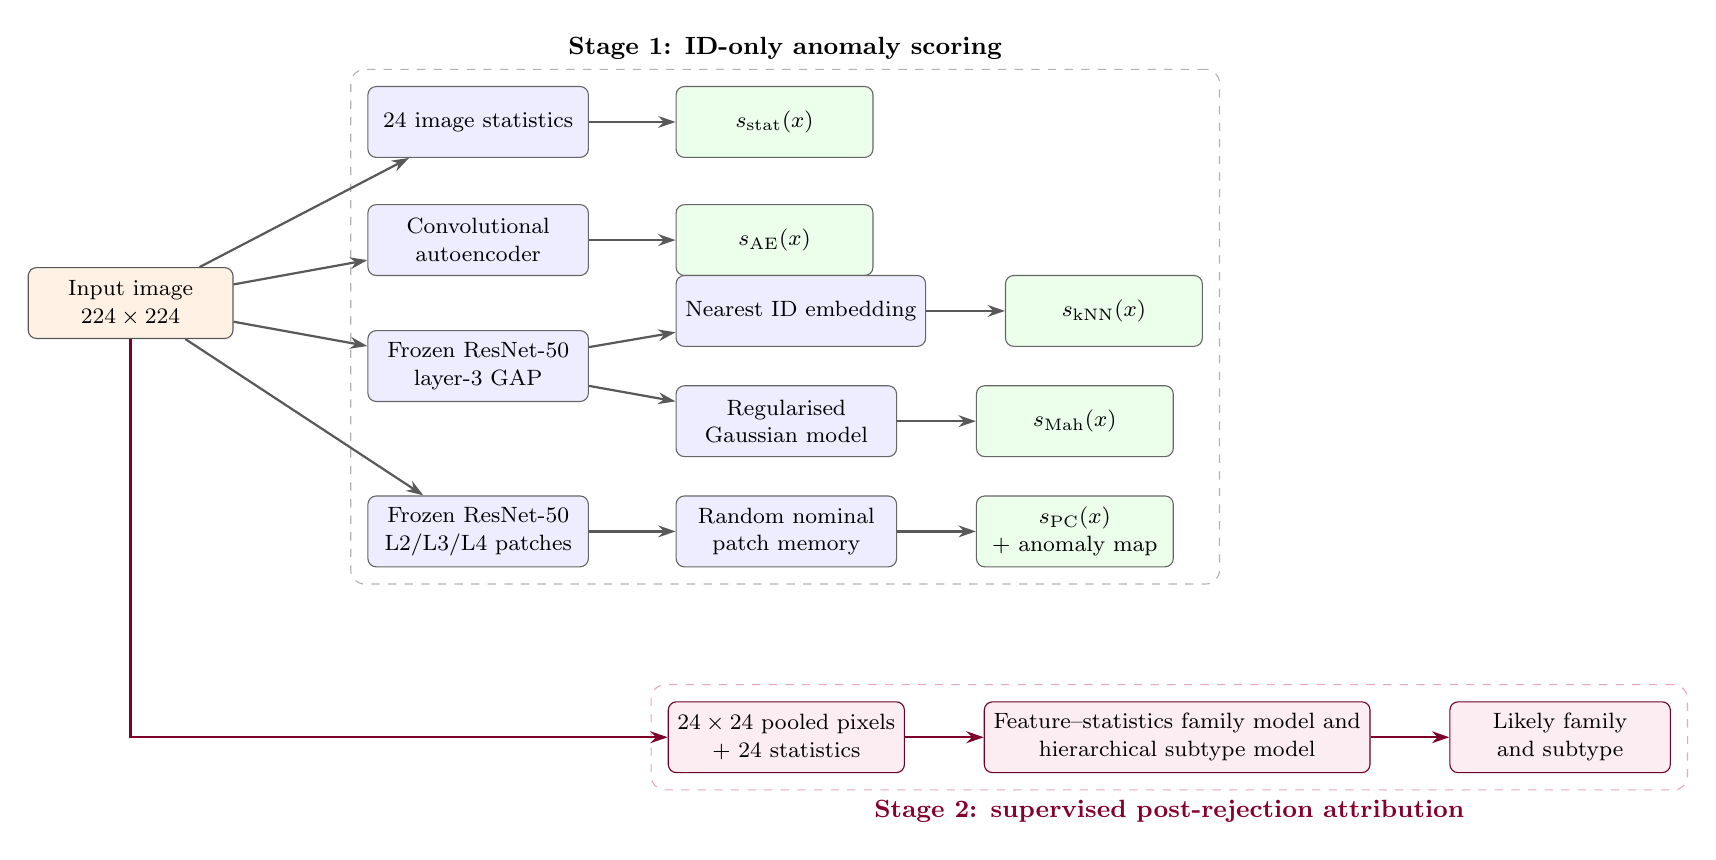
\begin{tikzpicture}[
        node distance=8mm and 11mm,
        every node/.style={font=\fontsize{8.5pt}{10pt}\selectfont},
        input/.style={
            rectangle,
            rounded corners=3pt,
            draw=black!65,
            fill=orange!10,
            minimum width=2.6cm,
            minimum height=0.9cm,
            align=center
        },
        process/.style={
            rectangle,
            rounded corners=3pt,
            draw=black!60,
            fill=blue!7,
            minimum width=2.8cm,
            minimum height=0.9cm,
            align=center
        },
        score/.style={
            rectangle,
            rounded corners=3pt,
            draw=black!60,
            fill=green!8,
            minimum width=2.5cm,
            minimum height=0.9cm,
            align=center
        },
        explain/.style={
            rectangle,
            rounded corners=3pt,
            draw=purple!60!black,
            fill=purple!7,
            minimum width=2.8cm,
            minimum height=0.9cm,
            align=center
        },
        arrow/.style={
            -{Stealth[length=2.2mm,width=1.5mm]},
            thick,
            draw=black!65
        },
        group/.style={
            rectangle,
            rounded corners=5pt,
            draw=black!30,
            dashed,
            inner sep=6pt
        }
    ]

    \node[input] (image) {Input image\\$224\times224$};

    \node[process, right=17mm of image, yshift=23mm] (stats)
        {24 image statistics};
    \node[score, right=11mm of stats] (statsscore)
        {$s_{\mathrm{stat}}(x)$};

    \node[process, right=17mm of image, yshift=8mm] (ae)
        {Convolutional\\autoencoder};
    \node[score, right=11mm of ae] (aescore)
        {$s_{\mathrm{AE}}(x)$};

    \node[process, right=17mm of image, yshift=-8mm] (cnn)
        {Frozen ResNet-50\\layer-3 GAP};
    \node[process, right=11mm of cnn, yshift=7mm] (knn)
        {Nearest ID embedding};
    \node[score, right=10mm of knn] (knnscore)
        {$s_{\mathrm{kNN}}(x)$};
    \node[process, right=11mm of cnn, yshift=-7mm] (mah)
        {Regularised\\Gaussian model};
    \node[score, right=10mm of mah] (mahscore)
        {$s_{\mathrm{Mah}}(x)$};

    \node[process, right=17mm of image, yshift=-29mm] (patch)
        {Frozen ResNet-50\\L2/L3/L4 patches};
    \node[process, right=11mm of patch] (memory)
        {Random nominal\\patch memory};
    \node[score, right=10mm of memory] (pcscore)
        {$s_{\mathrm{PC}}(x)$\\+ anomaly map};

    \node[explain, below=17mm of memory] (stage2feat)
        {$24\times24$ pooled pixels\\+ 24 statistics};
    \node[explain, right=10mm of stage2feat] (stage2model)
        {Feature--statistics family model and\\hierarchical subtype model};
    \node[explain, right=10mm of stage2model] (stage2out)
        {Likely family\\and subtype};

    \draw[arrow] (image) -- (stats);
    \draw[arrow] (stats) -- (statsscore);

    \draw[arrow] (image) -- (ae);
    \draw[arrow] (ae) -- (aescore);

    \draw[arrow] (image) -- (cnn);
    \draw[arrow] (cnn) -- (knn);
    \draw[arrow] (knn) -- (knnscore);
    \draw[arrow] (cnn) -- (mah);
    \draw[arrow] (mah) -- (mahscore);

    \draw[arrow] (image) -- (patch);
    \draw[arrow] (patch) -- (memory);
    \draw[arrow] (memory) -- (pcscore);

    \draw[arrow, purple!65!black] (image.south) |- (stage2feat.west);
    \draw[arrow, purple!65!black] (stage2feat) -- (stage2model);
    \draw[arrow, purple!65!black] (stage2model) -- (stage2out);

    \begin{scope}[on background layer]
        \node[group,
              fit=(stats)(statsscore)(ae)(aescore)(cnn)(knn)(knnscore)
                  (mah)(mahscore)(patch)(memory)(pcscore),
              label={[font=\bfseries\small]above:
              Stage~1: ID-only anomaly scoring}] {};
        \node[group,
              draw=purple!35,
              fit=(stage2feat)(stage2model)(stage2out),
              label={[font=\bfseries\small,text=purple!70!black]below:
              Stage~2: supervised post-rejection attribution}] {};
    \end{scope}

    \end{tikzpicture}%
    }
    \caption[Implemented Stage~1 and Stage~2 method pathways.]{Implemented
    methodological pathways. Stage~1 constructs anomaly
    scores from nominal training data only. Stage~2 is a separate supervised
    module used to attribute likely reasons after rejection.}
    \label{fig:methodology_overview}
\end{figure}

\subsection{Preprocessing and ID-Only Fitting}
\label{subsec:shared_preprocessing}

All inputs are resized deterministically to $224\times224$ pixels, and no
random augmentation is used during Stage~1 fitting or evaluation. The
image-statistics and autoencoder baselines operate on intensities scaled to
$[0,1]$. The autoencoder retains one channel. Feature-distance and PatchCore
methods convert each image to three identical greyscale channels and apply
ImageNet normalisation:

\begin{equation}
    x'_{c}(u,v)
    =
    \frac{x_{c}(u,v)-\mu_c}{\sigma_c},
    \qquad
    \boldsymbol{\mu}=(0.485,0.456,0.406),
    \quad
    \boldsymbol{\sigma}=(0.229,0.224,0.225).
    \label{eq:method_imagenet_normalisation}
\end{equation}

In Equation~\ref{eq:method_imagenet_normalisation},
$x_c(u,v)$ is the intensity at channel $c$ and pixel location $(u,v)$,
$x'_c(u,v)$ is the normalised intensity, and $\mu_c$ and $\sigma_c$ are the
ImageNet mean and standard deviation for channel $c\in\{1,2,3\}$. Although the
three input channels contain identical greyscale content, channel-specific
ImageNet normalisation is retained to match the pretrained backbone
convention.

For every Stage~1 method, fitting code retains ID rows only. Model parameters,
summary statistics, global memories, covariance estimates, and patch memories
are therefore functions solely of
$\mathcal{D}_{\mathrm{ID}}^{\mathrm{train}}$. OOD family and subtype labels do
not enter any Stage~1 scoring function.

\subsection{Image-Statistics Baseline}
\label{subsec:image_statistics_method}

The image-statistics detector tests whether low-level acquisition and intensity
properties already separate the benchmark. For an image $x$, it constructs

\begin{equation}
    \mathbf{h}(x)
    =
    \left[
        \mu_x,\,
        \sigma_x,\,
        x_{\min},\,
        x_{\max},\,
        H(x),\,
        E(x),\,
        F(x),\,
        B(x),\,
        \mathbf{p}(x)^{\top}
    \right]^{\top}
    \in\mathbb{R}^{24}.
    \label{eq:method_statistics_vector}
\end{equation}

Here, $\mathbf{h}(x)$ is the complete descriptor; $\mu_x$ and $\sigma_x$ are
the image mean and standard deviation; $x_{\min}$ and $x_{\max}$ are the
minimum and maximum intensities; $H(x)$ is histogram entropy; $E(x)$ is
finite-difference edge density; $F(x)$ is the fraction of pixels whose
intensity exceeds $\mu_x+0.25\sigma_x$; $B(x)$ is the fraction of pixels on
the outer image border with intensity at most $0.05$; and
$\mathbf{p}(x)\in\mathbb{R}^{16}$ is a normalised 16-bin intensity histogram.
The transpose symbol $(\cdot)^{\top}$ converts the concatenated entries into a
column vector.

For feature dimension $j\in\{1,\ldots,24\}$, the standardised deviation is

\begin{equation}
    \begin{aligned}
        \widehat{\sigma}^{\star}_j
        &=
        \begin{cases}
            \widehat{\sigma}_j, & \widehat{\sigma}_j\geq\varepsilon,\\
            1, & \widehat{\sigma}_j<\varepsilon,
        \end{cases}\\[2pt]
        \widetilde{h}_j(x)
        &=
        \frac{h_j(x)-\widehat{\mu}_j}{\widehat{\sigma}^{\star}_j}.
    \end{aligned}
    \label{eq:method_statistics_standardisation}
\end{equation}

In this expression, $h_j(x)$ is the $j$th component of $\mathbf{h}(x)$,
$\widehat{\mu}_j$ and $\widehat{\sigma}_j$ are the ID-training mean and
standard deviation of that component, and $\varepsilon>0$ defines the
near-zero-variance condition. The implementation uses
$\widehat{\sigma}^{\star}_j=1$ for such dimensions. The image-level score is

\begin{equation}
    s_{\mathrm{stat}}(x)
    =
    \sqrt{
        \frac{1}{D}
        \sum_{j=1}^{D}
        \widetilde{h}_j(x)^2
    },
    \qquad
    D=24.
    \label{eq:method_statistics_score}
\end{equation}

Here, $D$ is the descriptor dimensionality. The score is the root-mean-square
standardised distance from the nominal descriptor centre. It intentionally
ignores learned spatial semantics and serves as a transparent
low-complexity baseline.

\subsection{Autoencoder Reconstruction Baseline}
\label{subsec:autoencoder_method}

The reconstruction baseline is a convolutional autoencoder fitted on nominal
images only. For a one-channel $224\times224$ input, the encoder applies three
$3\times3$ convolutions with stride two and padding one:

\begin{equation}
    1\times224\times224
    \rightarrow
    16\times112\times112
    \rightarrow
    32\times56\times56
    \rightarrow
    64\times28\times28.
    \label{eq:method_ae_encoder_dimensions}
\end{equation}

Each triplet denotes channels, height, and width. Each encoder convolution is
followed by ReLU. The decoder mirrors this spatial reduction using three
$4\times4$ transposed convolutions with stride two and padding one:

\begin{equation}
    64\times28\times28
    \rightarrow
    32\times56\times56
    \rightarrow
    16\times112\times112
    \rightarrow
    1\times224\times224.
    \label{eq:method_ae_decoder_dimensions}
\end{equation}

The first two decoder layers use ReLU, while the output layer uses a sigmoid
to return intensities in $[0,1]$. For encoder
$f_{\theta}$ and decoder $g_{\phi}$,

\begin{equation}
    \widehat{x}
    =
    g_{\phi}\!\left(f_{\theta}(x)\right),
    \label{eq:method_ae_reconstruction}
\end{equation}

where $\theta$ and $\phi$ denote the trainable encoder and decoder parameters,
respectively, and $\widehat{x}$ denotes the reconstructed image. The network
minimises

\begin{equation}
    \mathcal{L}_{\mathrm{AE}}(\theta,\phi)
    =
    \frac{1}{N}
    \sum_{i=1}^{N}
    \frac{1}{P}
    \left\|
        x_i-g_{\phi}(f_{\theta}(x_i))
    \right\|_2^2,
    \label{eq:method_ae_objective}
\end{equation}

where $\mathcal{L}_{\mathrm{AE}}$ is the average training loss,
$P=224\times224$ is the number of pixels in each one-channel image, and
$\|\cdot\|_2$ is the Euclidean norm. Optimisation uses Adam with learning rate
$10^{-3}$, batch size 32, and 50 epochs. At inference,

\begin{equation}
    s_{\mathrm{AE}}(x)
    =
    \frac{1}{P}
    \left\|
        x-\widehat{x}
    \right\|_2^2.
    \label{eq:method_ae_score}
\end{equation}

The method assumes that the ID-trained autoencoder reconstructs nominal
FAF-like images more accurately than unsupported inputs. Because the residual
is averaged across all $P$ pixels, a spatially small artefact may contribute
only weakly to the image-level score.

\subsection{Frozen CNN Feature Representation}
\label{subsec:feature_representation}

Global feature-distance and PatchCore methods use a frozen ImageNet-pretrained
ResNet-50. For residual stage $\ell$,

\begin{equation}
    \mathbf{F}_{\ell}(x)
    \in
    \mathbb{R}^{C_{\ell}\times H_{\ell}\times W_{\ell}}
    \label{eq:method_feature_map}
\end{equation}

denotes the feature map of query image $x$, where $\ell$ indexes the residual
stage, $C_{\ell}$ is the number of feature channels, and
$H_{\ell}\times W_{\ell}$ is the spatial feature grid.
Table~\ref{tab:resnet_feature_dimensions} gives the implemented dimensions.

\begin{table}[htbp]
    \centering
    \caption[ResNet-50 stages used by the implemented methods.]{Frozen
    ResNet-50 feature stages used by the implemented methods.}
    \label{tab:resnet_feature_dimensions}

    \small
    \setlength{\tabcolsep}{8pt}
    \renewcommand{\arraystretch}{1.08}

    \begin{tabular}{@{}lccc@{}}
        \toprule
        \textbf{Stage} &
        \textbf{Channels $C_{\ell}$} &
        \textbf{Grid $H_{\ell}\times W_{\ell}$} &
        \textbf{Use} \\
        \midrule
        Layer~2 & 512  & $28\times28$ & PatchCore L2 and L2+L3 \\
        Layer~3 & 1024 & $14\times14$ & Global methods and PatchCore L3 \\
        Layer~4 & 2048 & $7\times7$   & PatchCore L4 \\
        \bottomrule
    \end{tabular}
\end{table}

No backbone parameter is updated on the dissertation dataset. The extracted
representations therefore remain generic ImageNet features rather than
retinally fine-tuned embeddings.

\subsection{Global Feature-Distance Detectors}
\label{subsec:global_feature_methods}

The global methods spatially average the layer-3 feature map:

\begin{equation}
    \mathbf{z}(x)
    =
    \operatorname{GAP}\!\left(\mathbf{F}_{3}(x)\right)
    =
    \frac{1}{H_3W_3}
    \sum_{u=1}^{H_3}
    \sum_{v=1}^{W_3}
    \mathbf{F}_{3}(x)_{:,u,v}
    \in\mathbb{R}^{1024}.
    \label{eq:method_global_pooling}
\end{equation}

Here, $\operatorname{GAP}$ denotes global average pooling, $u$ and $v$ index
spatial positions, and the colon selects all 1024 channels at location
$(u,v)$. The nominal embedding set is

\begin{equation}
    \mathcal{Z}_{\mathrm{ID}}
    =
    \left\{
        \mathbf{z}(x_i)
        \mid
        x_i\in\mathcal{D}_{\mathrm{ID}}^{\mathrm{train}}
    \right\}.
    \label{eq:method_id_embedding_set}
\end{equation}

Thus, $\mathcal{Z}_{\mathrm{ID}}$ contains one 1024-dimensional embedding for
each of the $N=700$ nominal training images.

\subsubsection{Global Feature $k$-Nearest Neighbours}
\label{subsubsec:global_knn}

The implemented global $k$-nearest-neighbour detector uses $k=1$ and
Euclidean distance:

\begin{equation}
    s_{\mathrm{kNN}}(x)
    =
    \min_{\mathbf{z}_i\in\mathcal{Z}_{\mathrm{ID}}}
    \left\|
        \mathbf{z}(x)-\mathbf{z}_i
    \right\|_2.
    \label{eq:method_global_knn_score}
\end{equation}

Here, $\mathbf{z}_i$ is a nominal reference embedding and
$s_{\mathrm{kNN}}(x)$ is the distance from the query embedding to its nearest
nominal neighbour. All 700 nominal embeddings are retained. The method is
non-parametric, although global pooling can attenuate evidence confined to a
small spatial region.

\subsubsection{Mahalanobis Feature Distance}
\label{subsubsec:mahalanobis}

The Mahalanobis detector models the first two moments of the nominal embedding
distribution:

\begin{align}
    \widehat{\boldsymbol{\mu}}
    &=
    \frac{1}{N}
    \sum_{i=1}^{N}
    \mathbf{z}(x_i),
    \label{eq:method_mahalanobis_mean}\\
    \widehat{\boldsymbol{\Sigma}}
    &=
    \frac{1}{N-1}
    \sum_{i=1}^{N}
    \left(
        \mathbf{z}(x_i)-\widehat{\boldsymbol{\mu}}
    \right)
    \left(
        \mathbf{z}(x_i)-\widehat{\boldsymbol{\mu}}
    \right)^{\top}.
    \label{eq:method_mahalanobis_covariance}
\end{align}

In these equations,
$\widehat{\boldsymbol{\mu}}\in\mathbb{R}^{1024}$ is the sample mean,
$\widehat{\boldsymbol{\Sigma}}\in\mathbb{R}^{1024\times1024}$ is the unbiased
sample covariance, and $(\cdot)^{\top}$ denotes vector transpose. Because the
embedding dimension is 1024 while $N=700$, the sample covariance is rank
deficient. The implementation therefore uses

\begin{equation}
    \widetilde{\boldsymbol{\Sigma}}
    =
    \widehat{\boldsymbol{\Sigma}}
    +
    \lambda\mathbf{I},
    \qquad
    \lambda=10^{-3},
    \label{eq:method_mahalanobis_regularisation}
\end{equation}

where $\lambda$ is the diagonal regularisation coefficient and
$\mathbf{I}\in\mathbb{R}^{1024\times1024}$ is the identity matrix. The
Moore--Penrose pseudoinverse is denoted by
$\widetilde{\boldsymbol{\Sigma}}^{+}$. The query score is

\begin{equation}
    s_{\mathrm{Mah}}(x)
    =
    \sqrt{
        \left(
            \mathbf{z}(x)-\widehat{\boldsymbol{\mu}}
        \right)^{\top}
        \widetilde{\boldsymbol{\Sigma}}^{+}
        \left(
            \mathbf{z}(x)-\widehat{\boldsymbol{\mu}}
        \right)
    }.
    \label{eq:method_mahalanobis_score}
\end{equation}

The resulting scalar accounts for correlations and unequal nominal variance
among feature dimensions. Directions with low nominal variance contribute
more strongly than equally sized deviations along highly variable
directions.

\subsection{PatchCore Memory-Bank Detection}
\label{subsec:patchcore_method}

PatchCore preserves spatially local representations. For selected stage
$\ell$, every feature-grid location defines

\begin{equation}
    \mathbf{p}_{\ell,u,v}(x)
    =
    \mathbf{F}_{\ell}(x)_{:,u,v}
    \in\mathbb{R}^{C_{\ell}},
    \label{eq:method_patch_embedding}
\end{equation}

where $(u,v)$ is the spatial grid location and
$\mathbf{p}_{\ell,u,v}(x)$ contains all $C_{\ell}$ channel values at that
location. For L2+L3, layer~3 is bilinearly resized to the $28\times28$
layer-2 grid and concatenated channel-wise:

\begin{equation}
    \mathbf{p}_{2+3,u,v}(x)
    =
    \left[
        \mathbf{F}_{2}(x)_{:,u,v};
        \operatorname{Up}_{28\times28}
        \!\left(
            \mathbf{F}_{3}(x)
        \right)_{:,u,v}
    \right]
    \in\mathbb{R}^{1536}.
    \label{eq:method_multilayer_patch_embedding}
\end{equation}

The semicolon denotes vector concatenation and
$\operatorname{Up}_{28\times28}$ denotes bilinear resizing to the layer-2
spatial grid. The complete nominal patch set is

\begin{equation}
    \mathcal{M}_{\mathrm{full}}
    =
    \bigcup_{x_i\in\mathcal{D}_{\mathrm{ID}}^{\mathrm{train}}}
    \left\{
        \mathbf{p}_{u,v}(x_i)
    \right\}_{u,v}.
    \label{eq:method_full_patch_memory}
\end{equation}

Here, $\bigcup$ denotes the union over all nominal training images and spatial
positions. To reduce storage and matching cost, a deterministic random subset
is sampled with seed 42:

\begin{equation}
    |\mathcal{M}|
    =
    \min
    \left(
        \left\lceil
            \rho|\mathcal{M}_{\mathrm{full}}|
        \right\rceil,
        M_{\max}
    \right),
    \qquad
    \rho=0.1,
    \quad
    M_{\max}=100\,000.
    \label{eq:method_patchcore_coreset_size}
\end{equation}

In Equation~\ref{eq:method_patchcore_coreset_size},
$|\cdot|$ denotes set cardinality, $\rho$ is the retained fraction,
$\lceil\cdot\rceil$ is the ceiling operator, and $M_{\max}$ is the memory cap.
The retained set $\mathcal{M}$ is a seeded random subset rather than the
greedy farthest-point coreset used in the original PatchCore formulation.

For a query patch $\mathbf{p}$, the local anomaly value is

\begin{equation}
    a(\mathbf{p})
    =
    \min_{\mathbf{m}\in\mathcal{M}}
    \left\|
        \mathbf{p}-\mathbf{m}
    \right\|_2,
    \label{eq:method_patch_anomaly_score}
\end{equation}

where $\mathbf{m}$ is a retained nominal memory vector and
$a(\mathbf{p})$ is the nearest-memory Euclidean distance. Let
$\mathcal{P}(x)$ denote the complete set of query patches for image $x$. The
image-level score is

\begin{equation}
    s_{\mathrm{PC}}(x)
    =
    \max_{\mathbf{p}\in\mathcal{P}(x)}
    a(\mathbf{p}).
    \label{eq:method_patchcore_image_score}
\end{equation}

Thus, $s_{\mathrm{PC}}(x)$ is determined by the most anomalous query patch.
Nearest-neighbour count is one and no additional PatchCore reweighting term is
applied. The spatial score map is

\begin{equation}
    \mathbf{A}(x)
    =
    \left[
        a\!\left(
            \mathbf{p}_{u,v}(x)
        \right)
    \right]_{u,v},
    \label{eq:method_patchcore_map}
\end{equation}

where $\mathbf{A}(x)$ preserves the feature-grid arrangement of the patch
distances. It is resized to the input resolution only for visualisation and is
not trained against a pixel-level mask.

Figure~\ref{fig:patchcore_implementation} shows the exact implementation flow.

\begin{figure}[htbp]
    \centering
    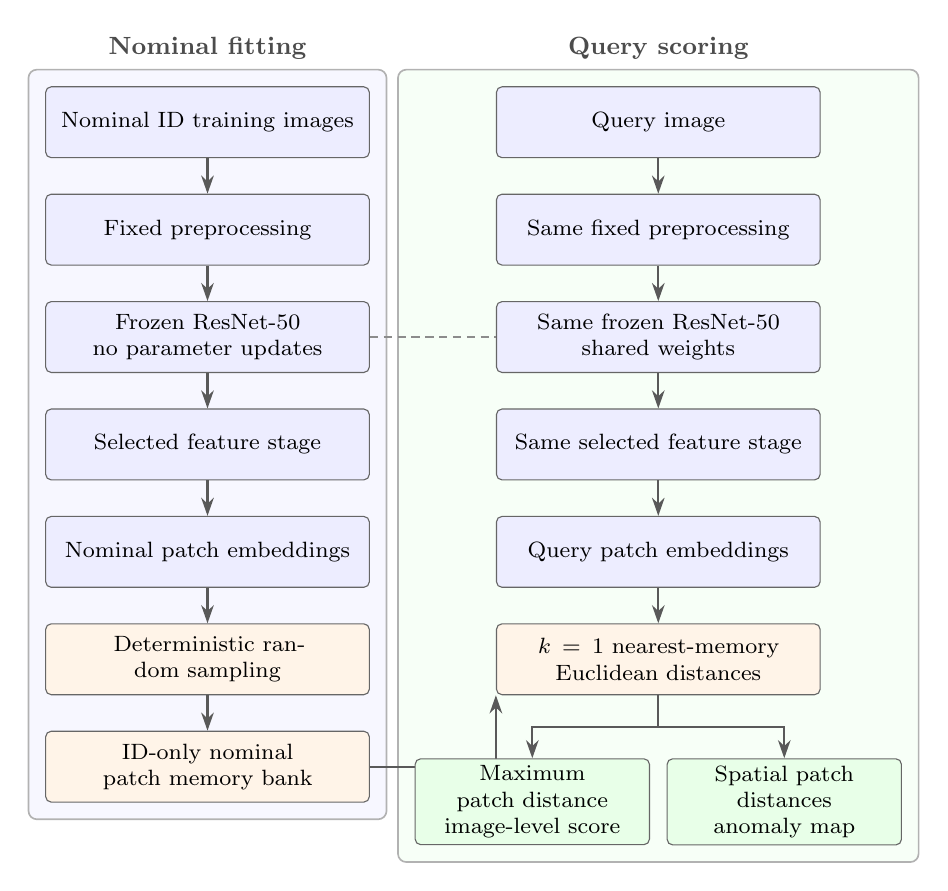
\begin{tikzpicture}[
        node distance=4.5mm and 16mm,
        every node/.style={font=\footnotesize},
        block/.style={
            rectangle,
            rounded corners=2pt,
            draw=black!60,
            fill=blue!7,
            minimum height=9mm,
            text width=39mm,
            align=center,
            inner sep=3pt
        },
        memory/.style={
            rectangle,
            rounded corners=2pt,
            draw=black!60,
            fill=orange!9,
            minimum height=9mm,
            text width=39mm,
            align=center,
            inner sep=3pt
        },
        output/.style={
            rectangle,
            rounded corners=2pt,
            draw=black!60,
            fill=green!9,
            minimum height=10mm,
            text width=28mm,
            align=center,
            inner sep=2.5pt
        },
        arrow/.style={
            -{Stealth[length=2.3mm,width=1.6mm]},
            line width=0.8pt,
            draw=black!65
        },
        shared/.style={densely dashed,line width=0.65pt,draw=black!45},
        group/.style={rounded corners=3pt,draw=black!30,line width=0.6pt,inner sep=6pt},
        annotation/.style={font=\footnotesize,text=black!70,align=center}
    ]
        % Nominal fitting path
        \node[block] (trainimg) {Nominal ID training images};
        \node[block, below=of trainimg] (trainprep) {Fixed preprocessing};
        \node[block, below=of trainprep] (trainbackbone)
            {Frozen ResNet-50\\no parameter updates};
        \node[block, below=of trainbackbone] (trainstage)
            {Selected feature stage};
        \node[block, below=of trainstage] (trainpatch)
            {Nominal patch embeddings};
        \node[memory, below=of trainpatch] (sampling)
            {Deterministic random sampling};
        \node[memory, below=of sampling] (bank)
            {ID-only nominal patch memory bank};

        \draw[arrow] (trainimg) -- (trainprep);
        \draw[arrow] (trainprep) -- (trainbackbone);
        \draw[arrow] (trainbackbone) -- (trainstage);
        \draw[arrow] (trainstage) -- (trainpatch);
        \draw[arrow] (trainpatch) -- (sampling);
        \draw[arrow] (sampling) -- (bank);

        % Query scoring path
        \node[block, right=of trainimg] (query) {Query image};
        \node[block, below=of query] (queryprep) {Same fixed preprocessing};
        \node[block, below=of queryprep] (querybackbone)
            {Same frozen ResNet-50\\shared weights};
        \node[block, below=of querybackbone] (querystage)
            {Same selected feature stage};
        \node[block, below=of querystage] (querypatch)
            {Query patch embeddings};
        \node[memory, below=of querypatch] (distance)
            {$k=1$ nearest-memory Euclidean distances};

        \draw[arrow] (query) -- (queryprep);
        \draw[arrow] (queryprep) -- (querybackbone);
        \draw[arrow] (querybackbone) -- (querystage);
        \draw[arrow] (querystage) -- (querypatch);
        \draw[arrow] (querypatch) -- (distance);
        \draw[arrow] (bank.east) -| (distance.south west);

        \coordinate (scorefork) at ($(distance.south)+(0,-4mm)$);
        \node[output, below=8mm of distance, xshift=-16mm] (imagescore)
            {Maximum patch distance\\image-level score};
        \node[output, below=8mm of distance, xshift=16mm] (map)
            {Spatial patch distances\\anomaly map};
        \draw[line width=0.8pt,draw=black!65] (distance.south) -- (scorefork);
        \draw[arrow] (scorefork) -| (imagescore.north);
        \draw[arrow] (scorefork) -| (map.north);

        \draw[shared] (trainbackbone.east) -- (querybackbone.west);

        \begin{scope}[on background layer]
            \node[group,fill=blue!3,fit=(trainimg)(bank),
                label={[font=\small\bfseries,text=black!70]above:Nominal fitting}] {};
            \node[group,fill=green!3,fit=(query)(distance)(imagescore)(map),
                label={[font=\small\bfseries,text=black!70]above:Query scoring}] {};
        \end{scope}
    \end{tikzpicture}
    \caption[ID-only PatchCore fitting and query scoring.]{
    \textbf{Implemented PatchCore workflow.} Nominal ID images pass through
    fixed preprocessing and a frozen ResNet-50; selected-stage patch
    embeddings are deterministically sampled to form the ID-only memory bank.
    Query patches use the same frozen representation and are scored by
    $k=1$ nearest-memory Euclidean distance; they are never added to the memory
    bank. The maximum patch distance is the image-level anomaly score, while
    the spatial distance arrangement forms the anomaly map.}
    \label{fig:patchcore_implementation}
\end{figure}

The four completed variants differ only in the selected feature stages:
L2, L3, L4, and L2+L3. Backbone, preprocessing, coreset ratio, memory cap,
nearest-neighbour rule, and maximum aggregation remain fixed.

The nearest-neighbour count $k=1$ was fixed before evaluation for both the
global $k$-NN detector and all PatchCore variants. It measures support from
the closest nominal reference while avoiding an additional tuned
neighbourhood-size hyperparameter. No $k$-ablation was performed, so the
setting is treated as a pre-specified implementation choice rather than an
empirically validated optimum; the test set was not used to choose $k$.

\subsection{Score-to-Decision Interface}
\label{subsec:threshold_interface}

All Stage~1 methods use the common interface defined in
Section~\ref{sec:system_design}, although their anomaly scores occupy
different numerical ranges. The scoring functions are defined in the preceding
sections, while ID-calibrated quantiles, retrospective operating points, and
threshold-conditioned evaluation are specified in
Section~\ref{sec:experimental_protocol}.

\subsection{Stage~2 Post-Rejection Attribution}
\label{subsec:stage2_methodology}

Stage~2 is a supervised, closed-set module applied after Stage~1 rejection. It
predicts an OOD family and, where applicable, a more specific subtype. It does
not use the Stage~1 anomaly score as an input and cannot alter the Stage~1
decision.

\paragraph{Image-derived representations.}
Two deterministic image representations are used. The first is the
24-dimensional statistics vector $\mathbf{h}(x)$ defined in
Equation~\ref{eq:method_statistics_vector}. The second converts the image to
greyscale, resizes it bilinearly to $24\times24$, scales the values to
$[0,1]$, and applies row-major flattening:

\begin{equation}
    \mathbf{r}(x)
    =
    \operatorname{vec}
    \left(
        \operatorname{Resize}_{24\times24}
        \left(
            \operatorname{Gray}(x)
        \right)
    \right)
    \in\mathbb{R}^{576}.
    \label{eq:method_stage2_pooled_pixels}
\end{equation}

The two representations are concatenated to form

\begin{equation}
    \mathbf{u}(x)
    =
    \left[
        \mathbf{r}(x);
        \mathbf{h}(x)
    \right]
    \in\mathbb{R}^{600},
    \label{eq:method_stage2_fusion}
\end{equation}

where the semicolon denotes concatenation. All Stage~2 inputs are derived from
image content. Metadata and target fields---including image paths, filenames,
source information, URLs, licence records, notes, labels, family and subtype
targets, transformations, severity values, hashes, and split identifiers---are
excluded. The Stage~1 anomaly score is also excluded.

\paragraph{Family attribution.}
The validation-selected family model applies a training-fitted
\texttt{StandardScaler} followed by balanced multinomial logistic regression
to $\mathbf{u}(x)$. The implementation uses the L-BFGS solver, $L_2$
regularisation with $C=1$, seed 42, and a maximum of 5,000 iterations. For
family $c\in\mathcal{C}$,

\begin{equation}
    \eta_c(x)
    =
    \boldsymbol{\beta}_c^{\top}
    \widetilde{\mathbf{u}}(x)
    +
    b_c,
    \qquad
    p_c(x)
    =
    \frac{\exp(\eta_c(x))}
         {\sum_{c'\in\mathcal{C}}\exp(\eta_{c'}(x))},
    \qquad
    \widehat{y}_{\mathrm{family}}
    =
    \arg\max_{c\in\mathcal{C}}
    p_c(x),
    \label{eq:method_stage2_family_logreg}
\end{equation}

where $\widetilde{\mathbf{u}}(x)$ is the training-standardised fusion vector,
$\boldsymbol{\beta}_c$ and $b_c$ are the learned parameters, and
$\mathcal{C}$ contains the three OOD families. The returned probabilities are
used as model confidence values and are not interpreted as clinically
calibrated probabilities.

A pre-specified confidence threshold $\gamma=0.50$ permits an
\textsc{Unknown} family output:

\begin{equation}
    \widehat{y}(x)
    =
    \begin{cases}
        \widehat{y}_{\mathrm{family}},
        &
        \displaystyle
        \max_{c\in\mathcal{C}} p_c(x)
        \geq \gamma,\\[3pt]
        \textsc{Unknown},
        &
        \displaystyle
        \max_{c\in\mathcal{C}} p_c(x)
        < \gamma.
    \end{cases}
    \label{eq:method_stage2_unknown}
\end{equation}

Here, $\widehat{y}(x)$ denotes the final thresholded family output.

\paragraph{Subtype attribution.}
Flat baselines predict one of the 11 subtype labels directly. The selected
method uses a hierarchical classifier:

\begin{equation}
    \widehat{y}_{\mathrm{family}}
    =
    f_{\mathrm{family}}
    \left(
        \mathbf{u}(x)
    \right),
    \qquad
    \widehat{y}_{\mathrm{subtype}}
    =
    f_{\widehat{y}_{\mathrm{family}}}
    \left(
        \mathbf{u}(x)
    \right).
    \label{eq:method_stage2_hierarchy}
\end{equation}

The first model predicts one of the three OOD families, after which the
corresponding family-specific branch predicts the subtype. Both levels use
training-fitted standardisation and balanced logistic regression with the same
solver and iteration limit. A family containing a single subtype uses a
constant-label estimator, and a global subtype model is retained as a fallback
when a family-specific branch is unavailable.

Validation and test samples are routed using the predicted family rather than
the ground-truth family. The reported hierarchy is therefore non-oracle and
includes any errors propagated from the family prediction.

\paragraph{Evaluation boundary.}
Detection, localisation, and attribution serve different functions in the
system. Stage~1 determines whether an input is supported by the ID reference.
PatchCore spatial anomaly maps visualise the distribution of patch-level
feature discrepancies, but they are not segmentation masks, causal
explanations, or clinical findings. Stage~2 assigns a likely operational
reason from the predefined taxonomy after rejection.

Stage~2 is evaluated separately on the labelled OOD test set so that
attribution performance can be measured independently of Stage~1 threshold
errors. Its metrics therefore describe standalone attribution rather than
end-to-end system performance. The taxonomy remains closed-set: unfamiliar
failures may be assigned to an existing category or returned as
\textsc{Unknown}, but Stage~2 does not extend the open-world detection
capability of Stage~1.

The next section defines the protocol used to fit, calibrate, and evaluate the
two stages.

\newpage
\section{Experimental Protocol}
\label{sec:experimental_protocol}

This section defines the procedures used to fit, calibrate, and evaluate the
methods described in Section~\ref{sec:methodology}. The protocol separates
nominal model construction, threshold calibration, retrospective OOD
evaluation, robustness analysis, and Stage~2 attribution. Stage~1 remains
ID-only throughout: labelled OOD examples are introduced only after anomaly
scores have been generated.

\subsection{Evaluation Workflow and Data Separation}
\label{subsec:evaluation_workflow}

Figure~\ref{fig:evaluation_paradigm} summarises the complete workflow.
Synthetic ID training images are used to construct each Stage~1 detector. A
disjoint ID validation split supports ID-calibrated threshold selection. The
synthetic ID fallback test set and the structured OOD benchmark are introduced
only after fitting and calibration. Robustness, threshold, and failure
analyses are then derived from the resulting held-out scores.

\begin{figure}[htbp]
    \centering
    \resizebox{0.96\textwidth}{!}{%
    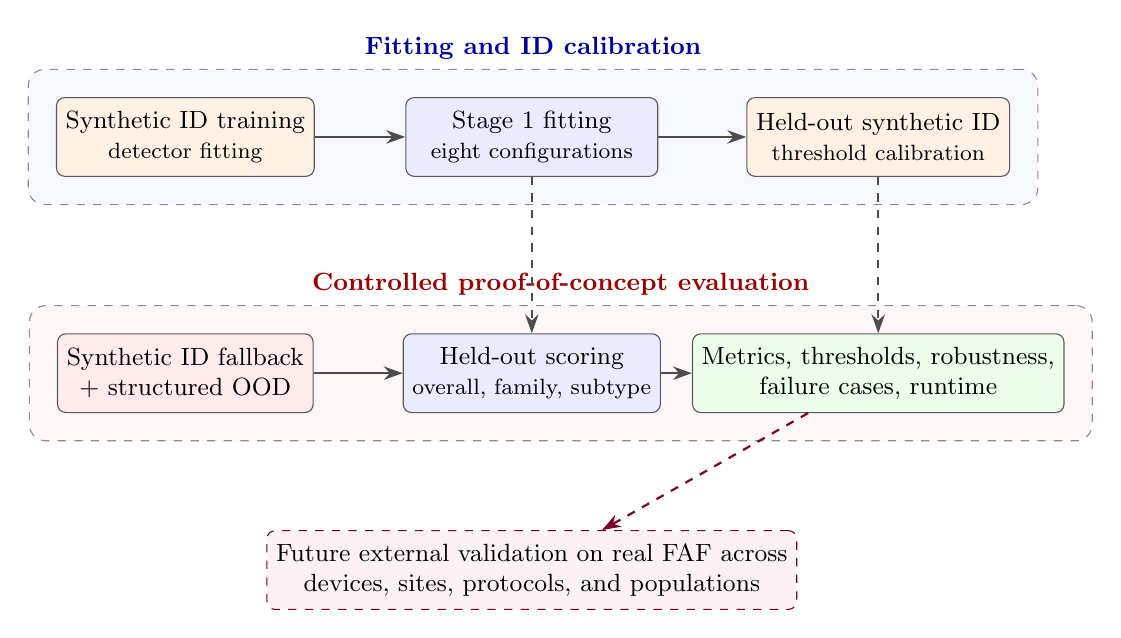
\begin{tikzpicture}[
        every node/.style={
            font=\fontsize{9pt}{10.8pt}\selectfont
        },
        phase/.style={
            rectangle,
            rounded corners=6pt,
            draw=black!45,
            dashed,
            inner sep=10pt
        },
        data/.style={
            rectangle,
            rounded corners=3pt,
            draw=black!65,
            fill=orange!10,
            minimum width=3.2cm,
            minimum height=1.0cm,
            align=center
        },
        process/.style={
            rectangle,
            rounded corners=3pt,
            draw=black!65,
            fill=blue!8,
            minimum width=3.2cm,
            minimum height=1.0cm,
            align=center
        },
        output/.style={
            rectangle,
            rounded corners=3pt,
            draw=black!65,
            fill=green!8,
            minimum width=3.4cm,
            minimum height=1.0cm,
            align=center
        },
        future/.style={
            rectangle,
            rounded corners=3pt,
            draw=purple!60!black,
            dashed,
            fill=purple!5,
            minimum width=4.6cm,
            minimum height=1.0cm,
            align=center
        },
        arrow/.style={
            -{Stealth[length=2.4mm,width=1.7mm]},
            thick,
            draw=black!70
        }
    ]

    \node[data] (train) at (0,0)
        {Synthetic ID training\\
         \footnotesize detector fitting};

    \node[process] (fit) at (4.4,0)
        {Stage~1 fitting\\
         \footnotesize eight configurations};

    \node[data] (val) at (8.8,0)
        {Held-out synthetic ID\\
         \footnotesize threshold calibration};

    \draw[arrow] (train) -- (fit);
    \draw[arrow] (fit) -- (val);

    \node[data, fill=red!8] (test) at (0,-3.0)
        {Synthetic ID fallback\\
         + structured OOD};

    \node[process] (score) at (4.4,-3.0)
        {Held-out scoring\\
         \footnotesize overall, family, subtype};

    \node[output] (analysis) at (8.8,-3.0)
        {Metrics, thresholds, robustness,\\
         failure cases, runtime};

    \draw[arrow] (test) -- (score);
    \draw[arrow] (score) -- (analysis);
    \draw[arrow, dashed] (fit) -- (score);
    \draw[arrow, dashed] (val) -- (analysis);

    \node[future] (clinical) at (4.4,-5.5)
        {Future external validation on real FAF across\\
         devices, sites, protocols, and populations};

    \draw[arrow, dashed, purple!65!black]
        (analysis) -- (clinical);

    \begin{scope}[on background layer]
        \node[
            phase,
            fill=blue!3,
            fit=(train)(fit)(val),
            label={[font=\bfseries\small,text=blue!60!black]above:
            Fitting and ID calibration}
        ] {};

        \node[
            phase,
            fill=red!3,
            fit=(test)(score)(analysis),
            label={[font=\bfseries\small,text=red!60!black]above:
            Controlled proof-of-concept evaluation}
        ] {};
    \end{scope}

    \end{tikzpicture}%
    }

    \caption[Experimental fitting, calibration, and evaluation workflow.]{
    Experimental workflow. Stage~1 fitting uses synthetic ID training
    images only. Held-out ID validation scores determine ID-calibrated
    thresholds, while the synthetic ID fallback and structured OOD sets are
    used for retrospective evaluation. External validation on real clinical
    FAF remains outside the present study.}
    \label{fig:evaluation_paradigm}
\end{figure}

The separation in Figure~\ref{fig:evaluation_paradigm} concerns data use, not
only file naming. OOD family and subtype labels are unavailable to every
Stage~1 fitting operation. They are consulted only after scoring, either to
compute retrospective metrics and stratified analyses or to define supervised
Stage~2 targets. The only threshold that uses OOD labels is the explicitly
research-only 95\% OOD-recall operating point described in
Section~\ref{subsec:threshold_policies}.

\subsection{Software Environment and Deterministic Execution}
\label{subsec:execution_environment}

The implementation uses Python, PyTorch and torchvision for neural feature
extraction, NumPy and pandas for numerical and tabular processing,
scikit-learn for metrics and Stage~2 classifiers, Pillow and OpenCV for image
operations, and Matplotlib for reporting. The repository records minimum
compatible dependency versions and the commands used to reproduce the
experiments.

All principal experiments use seed 42. The seed controls neural-network
initialisation, deterministic ID subset selection, PatchCore random-memory
sampling, bootstrap resampling, generated severity-test cases, and Stage~2
estimator initialisation. Evaluation data loaders do not shuffle samples, and
score files preserve manifest order so that every prediction remains
traceable to its source row.

The primary configurations select the available execution device
automatically. Runtime measurements use a local CPU path. Because the exact
processor model was not retained in the committed evidence, latency values
are interpreted as local engineering measurements rather than
hardware-independent benchmarks.

\subsection{Stage~1 Fitting, Calibration, and Test Isolation}
\label{subsec:stage1_fitting_calibration}

Each Stage~1 configuration is fitted using the 700-image nominal training
split. Image-statistics summaries, autoencoder parameters, global embedding
memories, covariance estimates, and PatchCore memories are therefore
constructed without access to the OOD benchmark.

The 150-image ID validation split is not merged with training. It is used only
to estimate ID score quantiles for threshold selection. The separate
150-image synthetic ID fallback test set remains held out until final scoring
and is used to estimate ID false rejection. It is not a substitute for a real
clinical FAF validation cohort.

The primary Stage~1 benchmark combines the 150 ID fallback images with 1,650
OOD images, comprising 150 examples from each of the 11 implemented subtypes.
This subtype-balanced view prevents the eight sensory-artefact subtypes from
dominating the comparison solely through their greater frequency. Supporting
analyses also use the full 2,100-image OOD set and the family-balanced set of
1,200 images, with 400 examples per OOD family.

All eight completed Stage~1 configurations are reported. No configuration is
removed after test inspection. Consequently, references to the ``strongest''
method or PatchCore layer describe retrospective performance on the stated
benchmark rather than selection verified on an independent external cohort.

\subsection{Stage~1 Evaluation Metrics}
\label{subsec:stage1_metrics}

OOD is treated as the positive class throughout Stage~1 evaluation, and larger
anomaly scores indicate stronger evidence for OOD. The analysis reports two
threshold-independent ranking metrics and two threshold-conditioned operating
measures.

AUROC summarises how consistently OOD images are ranked above ID images across
all possible thresholds. AUPRC summarises the precision--recall trade-off for
OOD detection. Because precision depends on class prevalence, AUPRC is
interpreted only with respect to the stated evaluation mixture, which is
OOD-heavy in the primary subtype-balanced benchmark.

For an operating threshold $\tau$, an image is rejected when $s_i\geq\tau$.
The corresponding ID false-rejection rate and OOD recall are

\begin{align}
    \operatorname{FRR}_{\mathrm{ID}}(\tau)
    &=
    \frac{
        \sum_{i:y_i=0}
        \mathbb{I}[s_i\geq\tau]
    }{
        \sum_i \mathbb{I}[y_i=0]
    },
    \label{eq:protocol_id_frr}\\[3pt]
    \operatorname{Recall}_{\mathrm{OOD}}(\tau)
    &=
    \frac{
        \sum_{i:y_i=1}
        \mathbb{I}[s_i\geq\tau]
    }{
        \sum_i \mathbb{I}[y_i=1]
    }.
    \label{eq:protocol_ood_recall}
\end{align}

Here, $s_i$ and $y_i\in\{0,1\}$ denote the anomaly score and binary label of
sample $i$, respectively, with $y_i=0$ for ID and $y_i=1$ for OOD.
$\mathbb{I}[\cdot]$ is the indicator function. The first quantity measures the
review burden imposed on nominal inputs, while the second measures the
proportion of benchmark OOD inputs rejected.

FPR@95\%TPR is reported as a research-oriented high-recall operating measure:

\begin{equation}
    \operatorname{FPR@95\%TPR}
    =
    \min_{\tau:
    \operatorname{Recall}_{\mathrm{OOD}}(\tau)\geq0.95}
    \operatorname{FRR}_{\mathrm{ID}}(\tau).
    \label{eq:protocol_fpr95}
\end{equation}

No interpolation beyond observed finite-sample thresholds is used. Because the
threshold is selected using labelled OOD evaluation data, FPR@95\%TPR is used
for retrospective method comparison rather than operational calibration.

\subsection{Threshold Policies and Provenance}
\label{subsec:threshold_policies}

Thresholds are divided according to the data used to determine them.

\paragraph{Research-only operating point.}
The research threshold is selected from labelled ID and OOD evaluation scores
to achieve at least 95\% empirical OOD recall while minimising ID false
rejection. Because it uses evaluation labels, it is reported only for
comparative analysis and is not treated as an operational calibration rule.

\paragraph{ID-calibrated quantile thresholds.}
Let the held-out ID validation scores for a method be

\begin{equation}
    \mathcal{S}_{\mathrm{ID}}^{\mathrm{val}}
    =
    \left\{
        s(x)
        \mid
        x\in\mathcal{D}_{\mathrm{ID}}^{\mathrm{val}}
    \right\}.
    \label{eq:protocol_validation_scores}
\end{equation}

For quantile $q\in(0,1)$, the threshold is

\begin{equation}
    \tau_q
    =
    Q_q
    \left(
        \mathcal{S}_{\mathrm{ID}}^{\mathrm{val}}
    \right),
    \label{eq:protocol_id_quantile}
\end{equation}

where $Q_q(\cdot)$ is the empirical $q$th quantile. The analysed values are
\[
    q\in\{0.95,0.975,0.99,0.995\}.
\]

\paragraph{Nominal rejection budgets.}
For a desired validation-ID rejection budget $\alpha\in(0,1)$,

\begin{equation}
    \tau_{\alpha}
    =
    Q_{1-\alpha}
    \left(
        \mathcal{S}_{\mathrm{ID}}^{\mathrm{val}}
    \right).
    \label{eq:protocol_rejection_budget}
\end{equation}

The evaluated rejection budgets are
\[
    \alpha\in\{0.05,0.10,0.20\}.
\]
The 5\% budget and the
95th-percentile policy are mathematically equivalent, but both descriptions
are retained because one emphasises quantile calibration and the other
emphasises expected nominal review burden.

The realised ID false-rejection rate on the fallback test set need not equal
the nominal validation budget exactly. Differences can arise from finite
validation size and from variation between the validation and fallback score
distributions.

\subsection{Stratified Stage~1 Evaluation}
\label{subsec:stratified_evaluation}

Aggregate results are supplemented by OOD family- and subtype-level analyses.
For each family, the corresponding OOD rows are paired with the same held-out
ID fallback set and the metrics are recomputed. The procedure is repeated for
all 11 subtypes. This preserves a common nominal reference while exposing
failure modes that may be hidden by overall averages.

Because the same 150 ID fallback images are reused across strata, the
family- and subtype-level estimates are statistically dependent. They are
used to characterise relative behaviour, not as independent hypothesis tests.
Score distributions and thresholded confusion counts are retained as
supporting evidence.

\subsection{Stage~2 Standalone Evaluation}
\label{subsec:stage2_evaluation_protocol}

Stage~2 uses the parent-grouped OOD-only splits defined in
Section~\ref{sec:dataset}. The 1,260-image training set fits all preprocessing
and attribution estimators, the 420-image validation set selects methods, and
the 420-image test set is not evaluated until both selections are frozen.
Every image derived from a shared parent is assigned with that parent to one
partition only. A non-empty parent-image hash defines the group when available;
otherwise the exact image path defines a singleton group. The final manifests
have zero shared image paths and zero shared normalised group identifiers
across training, validation, and test.

Family and subtype methods are selected by validation macro-F1. If methods are
tied within the implementation tolerance, the predefined lower-complexity
rank is preferred, followed by stable method-name ordering. Test performance
does not participate in the selection rule.

For $K$ classes, macro-F1 is

\begin{equation}
    \operatorname{MacroF1}
    =
    \frac{1}{K}
    \sum_{k=1}^{K}
    \frac{
        2\,\operatorname{Precision}_k
        \operatorname{Recall}_k
    }{
        \operatorname{Precision}_k
        +
        \operatorname{Recall}_k
    },
    \label{eq:protocol_macro_f1}
\end{equation}

with the standard convention that an undefined class-wise fraction is treated
according to the implementation's zero-division policy. Here, $K=3$ for
family attribution and $K=11$ for subtype attribution.

Family-level reporting includes accuracy, macro-F1, macro recall, class-wise
precision, recall and F1, known coverage, and the proportion assigned to
\textsc{Unknown}. Unknown predictions count as incorrect in headline accuracy
and macro-F1. The family confusion matrix uses the unthresholded argmax
prediction, so it visualises class-to-class confusion separately from
confidence-based abstention.

Subtype reporting includes accuracy, macro-F1, per-subtype precision, recall
and F1, and an 11-class confusion matrix. The hierarchical model uses predicted
rather than ground-truth family routing, so family errors propagate into the
subtype result.

Stage~2 evaluation is standalone: every labelled OOD test image is presented
to the attribution model. The resulting scores isolate attribution quality
and are not an end-to-end estimate of the subset that would reach Stage~2
after a particular Stage~1 threshold.

\subsection{Uncertainty and Training-Size Sensitivity}
\label{subsec:uncertainty_analysis}

Uncertainty in the principal Stage~1 metrics is estimated using a
sample-level percentile bootstrap with 500 valid replicates and seed 42. For
replicate $b\in\{1,\ldots,B\}$, where $B=500$, the combined evaluation rows
are sampled with replacement and the metric of interest is recomputed.
Replicates containing only one class are discarded because binary ranking
metrics are undefined.

If $\widehat{\theta}^{*(1)},\ldots,\widehat{\theta}^{*(B)}$ are the valid
bootstrap estimates of metric $\theta$, the two-sided 95\% percentile interval
is

\begin{equation}
    \operatorname{CI}_{0.95}(\theta)
    =
    \left[
        Q_{0.025}
        \left(
            \{\widehat{\theta}^{*(b)}\}_{b=1}^{B}
        \right),
        Q_{0.975}
        \left(
            \{\widehat{\theta}^{*(b)}\}_{b=1}^{B}
        \right)
    \right].
    \label{eq:protocol_bootstrap_ci}
\end{equation}

The resampling unit is the manifest row. These intervals therefore do not
correct for dependence among transformed images sharing the same parent.

Training-size sensitivity is evaluated for image statistics, global feature
kNN, and Mahalanobis distance using deterministic nominal subsets of
50, 100, 250, 500, and 700 images. Each detector is refitted at every size,
its threshold is recalibrated from the unchanged ID validation set, and it is
evaluated on the same primary benchmark. No OOD image enters refitting or
threshold calibration.

\subsection{Severity Stress Tests and Failure Analysis}
\label{subsec:robustness_failure_protocol}

Severity experiments examine whether anomaly scores change systematically as
controlled corruptions become stronger. Six artefact families are applied to
a deterministic subset of synthetic ID fallback images: blur, border crop,
Gaussian noise, JPEG compression, rectangle annotation, and text watermark.
Each artefact is generated at multiple predefined severity levels, with 12
images evaluated for each method--severity condition.

Previously fitted detectors are reused. For severity level $r$, the analysis
records mean and median anomaly score and rejection rates under both the
ID-calibrated and research-only thresholds. Monotonic association between
severity level and anomaly score is summarised by Spearman rank correlation:

\begin{equation}
    \rho_{\mathrm{S}}
    =
    \operatorname{corr}
    \left(
        \operatorname{rank}(r),
        \operatorname{rank}(s)
    \right),
    \label{eq:protocol_spearman}
\end{equation}

where $r$ denotes severity level and $s$ denotes the corresponding anomaly
score. This analysis tests controlled score response rather than clinical
artefact prevalence.

Failure analysis uses sample-level score tables. Mahalanobis distance is the
primary quantitative method, PatchCore L3 is the localisation-oriented
comparator, and the autoencoder and image-statistics baseline provide context.
Cases are grouped into ID false rejections, OOD misses, method-specific
successes, shared failures, and threshold-borderline cases. Within each group,
samples are ordered by absolute distance from the Mahalanobis threshold to
avoid choosing examples solely for visual effect.

A two-dimensional PCA projection of the Mahalanobis feature representation is
used only for qualitative inspection. PCA is fitted to evaluation embeddings,
and OOD labels are used only for colouring. The projection is not the
detector's decision space and does not contribute to any reported metric.

\subsection{Runtime and Resource Measurement}
\label{subsec:runtime_protocol}

Runtime is measured using a fixed 22-image smoke manifest on a local CPU path.
Each detector is loaded before timing. The timed interval includes manifest
construction, image loading, preprocessing, and score generation, but excludes
detector fitting and model loading.

For elapsed time $t_{\mathrm{elapsed}}$ seconds and
$n_{\mathrm{images}}$ scored images, latency is

\begin{equation}
    t_{\mathrm{image}}
    =
    \frac{
        1000\,t_{\mathrm{elapsed}}
    }{
        n_{\mathrm{images}}
    }
    \quad
    \text{ms/image}.
    \label{eq:protocol_runtime_per_image}
\end{equation}

Serialized model or reference size is measured from the saved artefact on
disk. It does not represent peak host or accelerator memory. Training time is
not reported because the robustness package reused existing fitted artefacts
rather than retraining every method under a common timing harness.

PatchCore L2+L3 is included in storage reporting, but its smoke-timing entry
uses the L3 scoring path to avoid a duplicate slow pass. It is therefore not
interpreted as an independent L2+L3 latency measurement.

\subsection{Reproducibility Controls and Statistical Reporting}
\label{subsec:protocol_reproducibility}

Every experiment is linked to explicit train, validation, and test manifests,
a version-controlled configuration, a fixed seed, a fitted artefact, and
sample-level score outputs. Tables and figures are generated from these score
files rather than transcribed manually. Dataset checksums and manifest audits
provide additional verification of input identity.

Stage~2 code records feature order and checks that file paths, hashes, source
metadata, split fields, and target labels are not concatenated into the model
input. Guard hashes verify that Stage~1 artefacts remain unchanged while
Stage~2 models are trained and evaluated.

Headline metrics are reported to four decimal places, while machine-readable
CSV files retain higher precision. Confusion matrices retain integer counts.
No null-hypothesis significance test is used because the study evaluates a
single synthetic-backed benchmark with known sample dependence.
Interpretation therefore emphasises effect sizes, confidence intervals,
stratified behaviour, threshold trade-offs, and observed failure cases.

The protocol does not remove the principal external-validity limitation:
training, calibration, and fallback ID testing remain synthetic. The reported
procedures constitute controlled proof-of-concept evaluation rather than
prospective clinical validation.

\newpage

\section{Experiments and Results}
\label{sec:results}

\begingroup
\setlength{\textfloatsep}{9pt plus 2pt minus 2pt}
\setlength{\floatsep}{8pt plus 2pt minus 2pt}
\setlength{\intextsep}{8pt plus 2pt minus 2pt}
\captionsetup{font=footnotesize,skip=4pt}

This section reports the results obtained under the protocol defined in
Section~\ref{sec:experimental_protocol}. Stage~1 results concern binary
input-validity detection under ID-only fitting, whereas Stage~2 results
concern supervised post-rejection attribution on labelled OOD data. Unless
otherwise stated, Stage~1 evaluation uses the subtype-balanced benchmark,
comprising 150 synthetic ID fallback images and 1,650 OOD images.

\subsection{Overall Stage~1 Performance}
\label{subsec:stage1_overall_results}

Table~\ref{tab:stage1_main_results} compares the five Stage~1 method families
and eight completed configurations. AUROC and AUPRC measure score ranking,
while FPR@95\%TPR quantifies the proportion of ID inputs rejected when at
least 95\% empirical OOD recall is required. The final column reports OOD
recall under a threshold calibrated solely from the held-out ID validation
set.

\begin{table}[H]
    \centering
    \caption[Overall Stage~1 performance.]
    {Overall Stage~1 performance on the subtype-balanced benchmark.}
    \label{tab:stage1_main_results}
    \footnotesize
    \setlength{\tabcolsep}{4pt}
    \renewcommand{\arraystretch}{1.02}
    \begin{tabularx}{0.88\textwidth}{@{}
        >{\raggedright\arraybackslash}X
        S[table-format=1.4]
        S[table-format=1.4]
        S[table-format=1.4]
        S[table-format=1.4]
    @{}}
        \toprule
        \textbf{Method} &
        {\textbf{AUROC}} &
        {\textbf{AUPRC}} &
        {\makecell[c]{\textbf{FPR@}\\\textbf{95\% TPR}}} &
        {\makecell[c]{\textbf{Recall at}\\$\boldsymbol{\tau}_{95}$}} \\
        \midrule
        \textbf{Mahalanobis feature} &
        \bfseries 0.9724 & \bfseries 0.9975 &
        \bfseries 0.2000 & \bfseries 0.9079 \\
        Global feature kNN & 0.9458 & 0.9949 & 0.3800 & 0.8024 \\
        PatchCore L3 & 0.8819 & 0.9880 & 0.6333 & 0.7097 \\
        PatchCore L2+L3 & 0.8722 & 0.9874 & 0.6867 & 0.6933 \\
        PatchCore L2 & 0.8280 & 0.9828 & 0.7867 & 0.6200 \\
        Image statistics & 0.7681 & 0.9717 & 0.7467 & 0.2994 \\
        Autoencoder & 0.7649 & 0.9763 & 0.9467 & 0.5588 \\
        PatchCore L4 & 0.7502 & 0.9692 & 0.8467 & 0.3527 \\
        \bottomrule
    \end{tabularx}
    \vspace{0.1em}
    \parbox{0.88\textwidth}{\scriptsize
    \emph{Note.} Higher values are better except FPR@95\% TPR;
    $\tau_{95}$ is the 95th percentile of held-out ID-validation scores.}
\end{table}

Mahalanobis feature distance produced the strongest overall result, achieving
AUROC 0.9724, AUPRC 0.9975, and FPR@95\%TPR 0.2000. Global feature kNN ranked
second on all three metrics. The two globally pooled feature-distance methods
therefore provided the strongest quantitative separation on the current
benchmark.

PatchCore L3 was the strongest patch-based configuration, with AUROC 0.8819,
but remained below both global feature methods. Combining layers~2 and~3 did
not improve performance, and the deeper L4 representation produced the
weakest PatchCore result. The image-statistics and autoencoder baselines
achieved similar AUROC values, although their threshold-conditioned behaviour
differed.

AUPRC was high for every method because OOD examples represented the large
majority of the primary evaluation set. Consequently, AUROC,
FPR@95\%TPR, and ID-calibrated recall provide the more discriminative
comparison. Complete ROC and precision--recall curves are provided in the
appendix.

\subsection{Stratified Performance and Method Complementarity}
\label{subsec:stage1_stratified_results}
\label{subsec:stage1_family_results}
\label{subsec:stage1_subtype_results}
\label{subsec:patchcore_results}

Aggregate results concealed substantial variation across OOD families.
Table~\ref{tab:stage1_family_auroc} is a stratified ranking analysis: each OOD
family is paired with the same 150-image synthetic ID fallback set, and AUROC
is reported to keep the comparison independent of family prevalence. The
four-metric summary in Table~\ref{tab:stage1_main_results} remains the primary
method comparison on the fixed subtype-balanced benchmark. AUPRC would change
with the family-specific OOD proportion, while a family-specific
FPR@95\%TPR would introduce a different threshold for each family. Recall at
the common ID-calibrated threshold is shown separately in
Figure~\ref{fig:appendix_family_threshold_recall}.

\begin{table}[H]
    \centering
    \caption[Stage~1 AUROC by OOD family.]
    {Family-level AUROC against the same synthetic ID reference.}
    \label{tab:stage1_family_auroc}
    \footnotesize
    \setlength{\tabcolsep}{4.2pt}
    \renewcommand{\arraystretch}{1.01}
    \begin{tabularx}{0.82\textwidth}{@{}
        >{\raggedright\arraybackslash}X
        S[table-format=1.4]
        S[table-format=1.4]
        S[table-format=1.4]
    @{}}
        \toprule
        \textbf{Method} &
        {\makecell[c]{\textbf{Modality}\\\textbf{shift}}} &
        {\makecell[c]{\textbf{Sensory}\\\textbf{artefact}}} &
        {\makecell[c]{\textbf{Semantic}\\\textbf{outlier}}} \\
        \midrule
        Mahalanobis feature & 1.0000 & 0.9621 & 1.0000 \\
        Global feature kNN & 1.0000 & 0.9255 & 1.0000 \\
        PatchCore L3 & 0.9822 & 0.8431 & 0.9918 \\
        PatchCore L2+L3 & 0.9919 & 0.8274 & 0.9912 \\
        PatchCore L2 & 0.9968 & 0.7719 & 0.9392 \\
        Image statistics & 0.9037 & 0.7056 & 0.9972 \\
        Autoencoder & 0.9927 & 0.6809 & 0.9809 \\
        PatchCore L4 & 0.8941 & 0.6878 & 0.9614 \\
        \bottomrule
    \end{tabularx}
\end{table}

Modality shifts and semantic outliers were separated almost perfectly by the
global feature-distance methods. Mahalanobis and global feature kNN both
achieved AUROC 1.0000 for these families. Sensory artefacts were consistently
more difficult because they retained the global appearance of the nominal
FAF-like images while modifying local content or low-level image properties.
Mahalanobis nevertheless remained strongest for this family, with AUROC
0.9621.

Table~\ref{tab:stage1_subtype_auroc_all} provides the complete
eight-method, eleven-subtype comparison. Values are rounded to two decimals for portrait
page layout; the generated result artefacts retain full precision.

\begin{table}[H]
    \centering
    \caption[Stage~1 AUROC by OOD subtype.]
    {Subtype AUROC for all eight Stage~1 configurations.}
    \label{tab:stage1_subtype_auroc_all}
    \label{tab:stage1_subtype_auroc_global}
    \label{tab:stage1_subtype_auroc_patchcore}
    \scriptsize
    \setlength{\tabcolsep}{2.7pt}
    \renewcommand{\arraystretch}{0.98}
    \begin{tabularx}{0.99\textwidth}{@{}
        >{\raggedright\arraybackslash}X
        *{8}{S[table-format=1.2]}
    @{}}
        \toprule
        & \multicolumn{4}{c}{\textbf{Global / reconstruction}} &
          \multicolumn{4}{c}{\textbf{PatchCore}} \\
        \cmidrule(lr){2-5}\cmidrule(l){6-9}
        \textbf{OOD subtype} &
        {\textbf{Stats}} & {\textbf{AE}} & {\textbf{kNN}} & {\textbf{Mah.}} &
        {\textbf{L2}} & {\textbf{L3}} & {\textbf{L4}} & {\textbf{L2+L3}} \\
        \midrule
        Colour fundus & 0.84 & 1.00 & 1.00 & 1.00 & 0.99 & 0.97 & 0.84 & 0.98 \\
        OCT screenshot & 0.97 & 0.99 & 1.00 & 1.00 & 1.00 & 0.99 & 0.95 & 1.00 \\
        Text watermark & 0.51 & 0.53 & 0.57 & 0.74 & 0.95 & 0.96 & 0.64 & 0.96 \\
        Rectangle annotation & 0.73 & 1.00 & 1.00 & 1.00 & 1.00 & 0.99 & 0.98 & 1.00 \\
        Arrow annotation & 0.71 & 1.00 & 0.96 & 1.00 & 1.00 & 1.00 & 0.99 & 1.00 \\
        Composite layout & 0.95 & 0.99 & 1.00 & 1.00 & 1.00 & 0.99 & 0.44 & 1.00 \\
        Blur & 0.65 & 0.11 & 0.99 & 1.00 & 0.49 & 0.58 & 0.59 & 0.55 \\
        Border crop & 0.70 & 0.43 & 0.96 & 0.99 & 0.75 & 0.88 & 0.74 & 0.89 \\
        Gaussian noise & 0.87 & 0.87 & 0.95 & 0.98 & 0.43 & 0.75 & 0.58 & 0.64 \\
        JPEG compression & 0.51 & 0.51 & 0.97 & 0.99 & 0.56 & 0.60 & 0.55 & 0.58 \\
        Natural image & 1.00 & 0.98 & 1.00 & 1.00 & 0.94 & 0.99 & 0.96 & 0.99 \\
        \bottomrule
    \end{tabularx}
    \vspace{0.1em}
    \parbox{0.99\textwidth}{\scriptsize
    \emph{Note.} Values are rounded to two decimals. Mah. denotes
    Mahalanobis feature distance.}
\end{table}

The full matrix shows why the aggregate ranking needs subtype context.
Mahalanobis achieved near-perfect separation for broad modality and semantic
shifts and remained strong for diffuse corruptions. Text watermark was its
main weakness, with AUROC 0.7361 at full precision. Global feature kNN followed
a similar pattern and reached only 0.5700 for text watermark.

PatchCore L3 reached AUROC 0.9572 for text watermark and exceeded 0.99 for
several annotation subtypes. Its lower scores for blur, Gaussian noise, and
JPEG compression indicate that the maximum local-patch distance responds
unevenly to diffuse changes. Layer~3 gave the strongest aggregate PatchCore
result, balancing local detail with higher-level structure. PatchCore therefore
contributes local evidence and spatial localisation alongside the stronger
global ranking of Mahalanobis.

Appendix~\ref{app:qualitative_subtype_analysis} provides paired-image
galleries covering all 11 subtypes, together with controlled-severity panels,
recorded false-negative cases, PatchCore localisation examples, and the full
ROC and precision--recall curves.

\subsection{Operating Points, Uncertainty, and Robustness}
\label{subsec:threshold_results}
\label{subsec:bootstrap_results}
\label{subsec:robustness_results}

The ranking metrics do not define a unique operating point.
Figure~\ref{fig:threshold_policy_tradeoff} therefore compares ID false
rejection and OOD recall under thresholds derived from held-out ID validation
scores and under the retrospective research-only threshold.

\begin{figure}[H]
    \centering
    \includegraphics[width=0.70\textwidth]
    {reports/dissertation_figures/compact/figure_threshold_policy_tradeoff.pdf}
    \caption[Threshold-policy trade-off.]
    {ID false rejection and OOD recall under ID-calibrated and
    research-only threshold policies.}
    \label{fig:threshold_policy_tradeoff}
\end{figure}

For Mahalanobis, the 95th-percentile ID-validation threshold was 38.5824. It
rejected 7 of 150 synthetic ID fallback images, corresponding to an ID
false-rejection rate of 0.0467, while rejecting 90.79\% of the OOD benchmark.
Increasing the threshold to the 97.5th and 99th validation percentiles reduced
ID false rejection to 0.0200 and 0.0133, but also reduced OOD recall to
0.8836 and 0.8727.

The research-only threshold achieved OOD recall 0.9503 but rejected 20.00\%
of the ID fallback set. This result illustrates why FPR@95\%TPR should be
treated as a comparative safety metric rather than a deployment threshold.

Threshold sensitivity was concentrated in sensory artefacts. Under the
95th-percentile Mahalanobis threshold, modality-shift and semantic-outlier
recall were both 1.0000, whereas sensory-artefact recall was 0.8733.
Text-watermark recall was only 0.1400. Lowering the threshold to the
research-only operating point raised watermark recall to 0.4667, but also
increased ID rejection by more than fourfold.

Table~\ref{tab:bootstrap_results} reports percentile bootstrap intervals for
the two principal Stage~1 configurations. The analysis used 500 sample-level
replicates with seed 42.

\begin{table}[H]
    \centering
    \caption[Bootstrap intervals for Stage~1 metrics.]
    {Bootstrap estimates with 95\% percentile intervals (500 replicates).}
    \label{tab:bootstrap_results}
    \scriptsize
    \setlength{\tabcolsep}{3.6pt}
    \renewcommand{\arraystretch}{1.02}
    \begin{tabularx}{0.92\textwidth}{@{}
        >{\raggedright\arraybackslash}p{2.45cm}
        >{\centering\arraybackslash}X
        >{\centering\arraybackslash}X
        >{\centering\arraybackslash}X
    @{}}
        \toprule
        \textbf{Method} &
        \textbf{AUROC (95\% CI)} &
        \textbf{AUPRC (95\% CI)} &
        \textbf{FPR@95\% TPR (95\% CI)} \\
        \midrule
        Mahalanobis feature &
        0.9724 (0.9638--0.9800) &
        0.9975 (0.9967--0.9983) &
        0.2000 (0.1061--0.2901) \\
        PatchCore L3 &
        0.8819 (0.8587--0.9013) &
        0.9880 (0.9847--0.9908) &
        0.6333 (0.5519--0.7110) \\
        \bottomrule
    \end{tabularx}
\end{table}

The AUROC and FPR@95\%TPR intervals remained separated, preserving the
ordering observed in the point estimates. These intervals quantify
sample-level uncertainty under the current benchmark, but do not account for
dependence among artefacts derived from shared parent images.

Training-size experiments indicated that the Mahalanobis result was not
already saturated at the smallest nominal subsets. Its AUROC increased from
0.9389 with 50 ID images to 0.9500 with 100, 0.9571 with 250, 0.9694 with
500, and 0.9724 with all 700 images. OOD recall under the recalibrated
95th-percentile threshold rose from 0.6830 to 0.9079 over the same range.
Global feature kNN followed the same broad trend, whereas the image-statistics
baseline varied non-monotonically.

Controlled severity experiments also revealed representation-dependent
behaviour. Mahalanobis scores were strongly associated with the severity of
blur, border crop, and Gaussian noise, with Spearman correlations of 0.9644,
0.9685, and 0.9268. Its watermark correlation was only 0.1776. PatchCore L3
showed stronger sensitivity to watermark severity
($\rho=0.5259$), but weaker monotonicity for JPEG compression
($\rho=0.1674$). Thus, increasing visual corruption did not produce a
uniform score response across methods or artefact types.

\subsection{Failure Patterns and Computational Cost}
\label{subsec:failure_results}
\label{subsec:runtime_results}

The deployment-style decisions exposed a clear complementarity between the
two principal methods. Mahalanobis rejected 90.79\% of the OOD benchmark and
falsely rejected 7 ID images, but detected only 14.00\% of text-watermark
examples. PatchCore L3 rejected 70.97\% of the benchmark and falsely rejected
10 ID images, but detected 85.33\% of text watermarks.

The opposite pattern occurred for diffuse corruptions. PatchCore L3 rejected
only 10.67\% of blur examples and 7.33\% of JPEG-compression examples at its
ID-validation threshold, whereas Mahalanobis was substantially more reliable
for blur, noise, crop, and compression. The global feature model was therefore
stronger for broad distributional changes, while the local patch model was
more responsive to visible overlays.

The baselines exhibited further distinct failures. The autoencoder separated
rectangle and arrow annotations almost perfectly in ranking terms, but
achieved AUROC 0.1116 for blur. Image statistics performed strongly on
semantic outliers but remained close to random ranking for text watermark
and JPEG compression. These results demonstrate that no single aggregate
metric fully characterises the operational failure surface.

Table~\ref{tab:runtime_results} reports local CPU smoke-test latency and
serialized artefact size. The timed region included image loading,
preprocessing, and score generation for 22 images, but excluded model loading
and fitting.

\begin{table}[H]
    \centering
    \caption[Local runtime and artefact size.]
    {Local CPU scoring cost and serialized artefact size.}
    \label{tab:runtime_results}
    \footnotesize
    \setlength{\tabcolsep}{4.5pt}
    \renewcommand{\arraystretch}{1.01}
    \begin{tabularx}{0.66\textwidth}{@{}
        >{\raggedright\arraybackslash}X
        S[table-format=2.4]
        S[table-format=2.4]
    @{}}
        \toprule
        \textbf{Method} &
        {\textbf{Size (MB)}} &
        {\textbf{ms/image}} \\
        \midrule
        Image statistics & 0.0013 & 11.5703 \\
        Autoencoder & 0.2553 & 10.9943 \\
        Global feature kNN & 2.5021 & 37.6755 \\
        Mahalanobis feature & 6.2061 & 39.3631 \\
        PatchCore L3 & 16.0489 & 55.8631 \\
        \bottomrule
    \end{tabularx}
    \vspace{0.1em}
    \parbox{0.66\textwidth}{\scriptsize
    \emph{Note.} Local 22-image CPU smoke test; values are not
    hardware-independent deployment benchmarks.}
\end{table}

The autoencoder and image-statistics baseline had the smallest stored
artefacts and lowest measured latency. Global feature kNN and Mahalanobis
incurred similar feature-extraction costs, while PatchCore L3 required a
larger memory bank and longer nearest-neighbour search.

Mahalanobis required 6.2061~MB and 39.3631~ms per image, compared with
16.0489~MB and 55.8631~ms per image for PatchCore L3. The L2+L3 PatchCore
artefact occupied 31.3294~MB, but an independent L2+L3 latency was not
recorded and is therefore not reported.

\subsection{Stage~2 Reason Attribution}
\label{subsec:stage2_method_results}
\label{subsec:stage2_family_results}
\label{subsec:stage2_subtype_results}

Stage~2 methods were selected using validation macro-F1 and subsequently
evaluated on the 420-image labelled OOD test split.
Table~\ref{tab:stage2_method_results} reports the resulting family- and
subtype-level performance.

\begin{table}[H]
    \centering
    \caption[Parent-grouped Stage~2 performance.]
    {Parent-grouped Stage~2 test performance after validation-only selection.}
    \label{tab:stage2_method_results}
    \scriptsize
    \setlength{\tabcolsep}{3.1pt}
    \renewcommand{\arraystretch}{1.01}
    \begin{tabularx}{0.92\textwidth}{@{}
        >{\raggedright\arraybackslash}X
        S[table-format=1.4]
        S[table-format=1.4]
        S[table-format=1.4]
        S[table-format=1.4]
    @{}}
        \toprule
        \textbf{Method} &
        {\makecell[c]{\textbf{Family}\\\textbf{acc.}}} &
        {\makecell[c]{\textbf{Family}\\\textbf{macro-F1}}} &
        {\makecell[c]{\textbf{Subtype}\\\textbf{acc.}}} &
        {\makecell[c]{\textbf{Subtype}\\\textbf{macro-F1}}} \\
        \midrule
        \textbf{Feature--statistics fusion}\textsuperscript{F} &
        \bfseries 1.0000 & \bfseries 1.0000 & 0.9048 & 0.8777 \\
        \textbf{Hierarchical classifier}\textsuperscript{S} &
        1.0000 & 1.0000 & \bfseries 0.9357 & \bfseries 0.9176 \\
        Random forest & 0.9976 & 0.9979 & 0.8310 & 0.7696 \\
        Logistic regression & 1.0000 & 1.0000 & 0.7619 & 0.6937 \\
        Linear SVM & 0.9976 & 0.9963 & 0.6929 & 0.6133 \\
        Global feature kNN & 0.9714 & 0.9676 & 0.6548 & 0.5430 \\
        Image-statistics logistic regression & 0.9452 & 0.9405 & 0.9095 & 0.8861 \\
        Nearest centroid & 0.8024 & 0.7735 & 0.5643 & 0.4499 \\
        \bottomrule
    \end{tabularx}
    \vspace{0.1em}
    \parbox{0.92\textwidth}{\scriptsize
    \emph{Note.} F and S identify the validation-selected family and subtype
    models. Bold family values mark the selected family model.}
\end{table}

\begin{figure}[H]
    \centering
    \includegraphics[width=0.86\textwidth]
    {reports/dissertation_figures/compact/figure_grouped_stage2_method_comparison.pdf}
    \caption[Parent-grouped Stage~2 candidate comparison.]
    {Validation and test macro-F1 across the eight Stage~2 candidates;
    selection used validation macro-F1.}
    \label{fig:stage2_grouped_method_comparison}
\end{figure}

The feature--statistics fusion logistic-regression model was selected for
family attribution because its
validation macro-F1 of 0.9925 was maximal under the predefined selection and
tie-breaking rule. Retrospective grouped-test accuracy, macro-F1, and balanced
accuracy were all 1.0000. Known-class coverage was 1.0000, with no unknown
outputs at the pre-specified confidence threshold.

Table~\ref{tab:stage2_family_confusion} reports its unthresholded argmax
confusion matrix. All 420 grouped-test images were classified correctly.

\begin{center}
    \begin{minipage}[t]{0.37\textwidth}
        \captionsetup{type=table,font=footnotesize,skip=3pt}
        \captionof{table}[Grouped-test family confusion matrix.]
        {Grouped-test family confusion matrix.}
        \label{tab:stage2_family_confusion}
        \centering
        \scriptsize
        \setlength{\tabcolsep}{2.4pt}
        \renewcommand{\arraystretch}{1.02}
        \begin{tabular}{@{}
            l
            S[table-format=3.0]
            S[table-format=3.0]
            S[table-format=3.0]
        @{}}
            \toprule
            \textbf{True} &
            {\textbf{Mod.}} &
            {\textbf{Art.}} &
            {\textbf{Sem.}} \\
            \midrule
            Modality & 80 & 0 & 0 \\
            Artefact & 0 & 240 & 0 \\
            Semantic & 0 & 0 & 100 \\
            \bottomrule
        \end{tabular}

        \vspace{0.2em}
        \raggedright\scriptsize
        Mod., Art., and Sem. denote modality shift, sensory artefact,
        and semantic outlier.
    \end{minipage}
    \hfill
    \begin{minipage}[t]{0.59\textwidth}
        \captionsetup{type=figure,font=footnotesize,skip=3pt}
        \centering
        \includegraphics[width=0.92\linewidth]
        {reports/dissertation_figures/compact/figure_grouped_subtype_confusion_matrix.pdf}
        \captionof{figure}[Grouped-test subtype confusion matrix.]
        {Grouped-test subtype confusion matrix for the selected non-oracle
        hierarchy; routing uses the predicted family.}
        \label{fig:stage2_grouped_subtype_confusion}
    \end{minipage}
\end{center}

All three family classes achieved F1 1.0000, so there was no unique hardest
family on this grouped test allocation. This perfect retrospective result did
not participate in model selection and should not be interpreted as clinical
generalisability.

The selected non-oracle hierarchical classifier achieved validation subtype
macro-F1 0.9059, followed by grouped-test accuracy 0.9357 and macro-F1 0.9176.
It outperformed the image-statistics classifier, which achieved test accuracy
0.9095 and macro-F1 0.8861, and the flat fusion classifier, which achieved
0.9048 and 0.8777.

Colour fundus, OCT screenshot, composite layout, border crop, Gaussian noise,
and natural-image content were classified without error. Text watermark was
the hardest subtype, with F1 0.7742 and 24 correct predictions from 30
examples. Arrow and rectangle annotations achieved F1 0.8000 and 0.8070,
respectively; JPEG compression achieved F1 0.8254.



The Stage~2 values remain standalone attribution results on labelled OOD data;
they do not represent end-to-end performance on only those images rejected by
a particular Stage~1 threshold.

Relative to the legacy row-stratified evaluation, grouped family validation
macro-F1 changed by $+0.0017$, family test accuracy by $+0.0119$, and family
test macro-F1 by $+0.0099$. Subtype validation macro-F1 changed by $+0.0387$,
test accuracy by $+0.0119$, and test macro-F1 by $+0.0116$. The increases show
that the allocation of parent groups changes benchmark difficulty; they do not
show that parent dependence improved the legacy estimates or that the model
generalises clinically.

\begin{figure}[!t]
    \centering
    \includegraphics[width=0.80\textwidth]
    {reports/dissertation_figures/compact/figure_legacy_vs_grouped_stage2_metrics.pdf}
    \caption[Legacy and parent-grouped Stage~2 comparison.]
    {Legacy row-stratified and final parent-grouped Stage~2 metrics;
    grouped results provide the headline evidence.}
    \label{fig:stage2_legacy_grouped_comparison}
\end{figure}

\subsection{Summary of Empirical Findings}
\label{subsec:results_summary}

Mahalanobis feature distance was the strongest quantitative Stage~1 detector
on the present benchmark and offered a favourable balance between ranking
performance, ID-calibrated recall, storage, and runtime. PatchCore L3 was the
strongest patch-based configuration and provided complementary sensitivity
to local overlays, particularly text watermarks, together with spatial
localisation evidence.

The results also show that the apparent strength of Stage~1 depends on the OOD
family, subtype, and selected threshold. Modality shifts and semantic outliers
were comparatively easy, whereas subtle sensory artefacts produced the
largest overlap with nominal inputs. Stage~2 achieved high family-level
attribution and lower, but still substantial, subtype-level performance. The
interpretation and external-validity limitations of these findings are
examined in Section~\ref{sec:discussion}.

\clearpage
\endgroup

\section{Discussion}
\label{sec:discussion}

This study examined whether an unsupervised, ID-only gatekeeper could identify
unsupported inputs before they reach a downstream retinal-imaging system.
Within the scope of the present synthetic-backed benchmark, the findings
support an affirmative answer to the primary research question: an ID-only
detector can reject a high proportion of the represented OOD inputs while
retaining most held-out synthetic nominal inputs under an ID-calibrated
threshold. Globally pooled feature-distance methods provided the strongest
Stage~1 separation, with Mahalanobis distance performing best overall.
PatchCore L3 was weaker in aggregate but supplied complementary sensitivity to
local overlays and spatial anomaly maps. Stage~2 further showed that many
rejected inputs could receive a plausible operational explanation, although
this attribution task remained supervised, closed-set, and methodologically
separate from Stage~1. These conclusions establish benchmark-level feasibility
rather than clinical effectiveness.

\subsection{Mahalanobis Provides the Strongest Overall Separation}
\label{subsec:discussion_stage1}

Regularised Mahalanobis distance on globally pooled, frozen ResNet-50 embeddings produced the strongest Stage~1 result, indicating that the main benchmark separations are represented in generic deep features. Covariance scaling emphasises deviations along stable nominal directions, which is consistent with its advantage over unweighted global kNN, although the experiment does not isolate covariance modelling as the sole cause.

Global kNN ranked second with a similar family profile, showing that the frozen representation itself contributed substantially. Both global methods captured broad modality and semantic shifts but were less sensitive to some local overlays.

Image statistics detected broad changes in intensity, entropy, borders, and histograms but lacked learned retinal structure and spatial specificity. The autoencoder could reconstruct unsupported low-level appearances well, so reconstruction error was not a reliable proxy for nominal support across all corruptions.

PatchCore L3 was the strongest patch-based configuration. Local patch comparison preserved watermark and annotation evidence that global pooling could dilute, while the maximum-patch score responded less consistently to diffuse blur and compression. Layer~3 provided the best balance of spatial detail and abstraction; layer~2 was less discriminative, layer~4 was coarser, and L2+L3 increased memory without improving aggregate performance.

\subsection{Global and Local Detectors Capture Complementary Failures}
\label{subsec:discussion_complementarity}

No detector dominated every subtype. Mahalanobis was strongest for modality
shift, semantic outliers, blur, crop, Gaussian noise, and JPEG compression.
PatchCore L3 was markedly stronger for text watermark and retained high scores
for several annotation subtypes. The aggregate AUROC ranking therefore captures
only part of the operating behaviour. Mahalanobis provides the strongest
general ranking on this benchmark, while PatchCore supplies local evidence for
spatially confined deviations.

\paragraph{Spatial anomaly maps.}
The term \emph{map} in this dissertation refers to a PatchCore spatial anomaly
map. Each query patch receives its Euclidean distance to the nearest nominal
memory-bank patch. These distances are placed back on the feature grid and
interpolated to image resolution, producing a heatmap of detector-relative
spatial discrepancy. The heatmap can draw attention to an annotation, border,
or local corruption during manual review. Its resolution is limited by the
feature stride and interpolation, and no pixel-level masks were used for
training or evaluation.

\paragraph{Spatial attribution for Mahalanobis.}
The implemented Mahalanobis detector uses a globally pooled layer-3 embedding,
so the current score contains no retained spatial coordinates. A spatial
extension is technically feasible. One option is to compute the gradient of
the scalar Mahalanobis score with respect to the final convolutional feature
map and form a Grad-CAM-style attribution \cite{selvaraju2017grad}. A more
direct distance-based alternative would estimate position-wise Gaussian
statistics on unpooled feature maps, following the local modelling principle
used by PaDiM \cite{defard2021padim}. Both approaches would require separate
validation because gradient attribution and local feature distance answer a
different question from the current global score. Their maps would also need
assessment against human review or region-level annotations before any claim
of reliable localisation.

\paragraph{Detector ensembles.}
The subtype matrix suggests useful complementarity between Mahalanobis and
PatchCore. A conservative ID-only ensemble could standardise each detector by
its held-out ID score distribution and reject when either calibrated score
exceeds its threshold. Score averaging, maximum normalised score, and a
sequential rule with Mahalanobis first and PatchCore as a local-artifact check
are further candidates. Conventional boosting would require labelled positive
and negative examples, changing Stage~1 into a supervised or semi-supervised
system. Any learned fusion therefore needs a separate validation set and an
evaluation containing previously unseen OOD mechanisms. The present results
motivate this analysis but do not establish that fusion improves external
generalisation.

\subsection{Threshold Choice Determines the Recall--Rejection Trade-off}
\label{subsec:discussion_thresholds}

Ranking performance does not determine an operating threshold. The 95th-percentile Mahalanobis policy rejected 4.67\% of synthetic ID fallback images and 90.79\% of OOD inputs; a lower research-only threshold raised OOD recall to about 95\% but increased ID rejection to 20\%. False rejection creates review or reacquisition burden, while false acceptance passes unsupported inputs downstream. Because these workflow costs were not measured, the ID-calibrated threshold is a transparent prototype policy rather than a clinical operating point.

FPR@95\%TPR is useful for comparing methods at a common high-recall target,
but its threshold is selected using labelled OOD evaluation data. It is
therefore a retrospective comparison measure, not a rule that can be
calibrated directly in an open-world setting. ID-validation quantiles require
only nominal data and are operationally more realistic, although their
realised false-rejection rate will depend on how closely the deployment
distribution matches the calibration set.

AUPRC also requires care because the primary benchmark is strongly OOD-heavy.
Its values are informative for comparison within this evaluation mixture but
should not be interpreted as estimates of real-world precision. AUROC,
ID-calibrated false rejection, OOD recall, and family- or subtype-level
results together provide a more informative assessment than any single
metric.

\subsection{Benchmark Robustness Coexists with Distinct Failure Modes}
\label{subsec:discussion_robustness}

Bootstrap intervals preserved the Mahalanobis--PatchCore ordering, although
they remain descriptive because rows generated from the same parent image are
dependent. Training-size analysis showed continued improvement in
Mahalanobis performance from 50 to 700 nominal images. This supports the
collection of a broader nominal reference set, but does not establish
performance on real FAF acquired across devices and sites.

Severity experiments showed that anomaly scores are not universally monotonic
measures of visible corruption strength. Mahalanobis responded strongly to
increasing blur, border crop, and Gaussian noise, but weakly to watermark
severity. PatchCore was more responsive to watermark strength and less
monotonic for JPEG compression. The two methods therefore encode different
forms of deviation, making a single method-independent interpretation of
severity inappropriate.

The stratified results further clarified these differences. Colour fundus
images produced broad acquisition and colour shifts, while OCT screenshots
introduced globally visible modality and layout changes. These properties
favoured global feature methods, although preserved retinal anatomy could make
some modality-shifted inputs more challenging. Natural images were generally
distant from the FAF reference in both structure and semantics, explaining
their strong separation across methods.

Local artefacts produced a different pattern. PatchCore performed strongly on
text watermarks because patch-level comparison retained small spatial
discrepancies that could be diluted by global pooling. Rectangle annotations
were usually distinctive because of their geometric edges, whereas small
arrows could overlap with retinal vessels and other existing edge structures.
Composite layouts affected both global organisation and local boundaries,
which explains the strong performance of global methods and shallower
PatchCore representations.

Diffuse corruptions were better captured by global feature distance.
Mahalanobis performed strongly on blur, border crop, Gaussian noise, and JPEG
compression because these transformations altered the pooled representation
across a substantial portion of the image. Mild blur and high-quality
compression were more difficult for PatchCore because many patches could
change moderately without producing one extreme local distance. Border crops
also altered field-of-view statistics, while distributed Gaussian noise
shifted the global embedding. The autoencoder's poor blur ranking suggests
that reconstruction error may decrease when smoothing removes
high-frequency structure that is difficult to reproduce.

Table~\ref{tab:subtype_method_interpretation} summarises the strongest observed
method patterns and the principal challenge associated with each subtype.
These patterns are post-hoc interpretations of the implemented
representations and should not be treated as independently validated causal
mechanisms.

\begin{table}[htbp]
    \centering
    \caption[Subtype-level detector patterns and challenges.]
    {Strongest observed detector patterns and principal challenges by OOD
    subtype.}
    \label{tab:subtype_method_interpretation}

    \footnotesize
    \setlength{\tabcolsep}{4pt}
    \renewcommand{\arraystretch}{1.05}

    \begin{tabularx}{0.92\textwidth}{@{}
        >{\raggedright\arraybackslash}p{3.0cm}
        >{\raggedright\arraybackslash}p{4.15cm}
        >{\raggedright\arraybackslash}X
    @{}}
        \toprule
        \textbf{Subtype} &
        \textbf{Strongest method(s)} &
        \textbf{Principal challenge} \\
        \midrule

        Colour fundus &
        Global methods; PatchCore L2 &
        Preserved retinal anatomy \\

        OCT screenshot &
        All methods &
        Cropped or simplified layouts \\

        \addlinespace[0.12em]

        Text watermark &
        PatchCore variants &
        Small or low-opacity text \\

        Rectangle annotation &
        AE, global methods, PatchCore &
        Thin or low-contrast boxes \\

        Arrow annotation &
        Mahalanobis; PatchCore &
        Small arrows near retinal vessels \\

        Composite layout &
        Global methods; shallow PatchCore &
        Subtle borders or small insets \\

        Blur &
        Mahalanobis; kNN &
        Mild and spatially diffuse blur \\

        Border crop &
        Mahalanobis; kNN &
        Narrow field-of-view changes \\

        Gaussian noise &
        Mahalanobis &
        Low-amplitude distributed noise \\

        JPEG compression &
        Mahalanobis; kNN &
        High-quality compression \\

        \addlinespace[0.12em]

        Natural image &
        All methods &
        Retinal-like monochrome textures \\

        \bottomrule
    \end{tabularx}
\end{table}

\subsection{Stage~2 Adds Useful but Closed-Set Rejection Explanations}
\label{subsec:discussion_stage2}

Stage~2 was stronger at family than subtype attribution. The selected fusion model separated all three families on the grouped test allocation, while hierarchical subtype routing outperformed flat pooled-pixel alternatives. Routing used the predicted family, so errors propagated without oracle information. Because evaluation used all labelled OOD test images, the metrics describe standalone attribution rather than end-to-end performance after a particular Stage~1 threshold.

The remaining subtype confusions were consistent with limitations of the
chosen representation. Rectangle and arrow annotations shared related
geometric structure, while text watermark, blur, and JPEG compression could
produce overlapping local or high-frequency changes. The pooled-pixel and
image-statistics features capture broad appearance efficiently but do not
preserve all fine spatial information needed for precise subtype distinction.

The parent-grouped score did not fall below the legacy row-level result. This
does not invalidate the original leakage concern: regrouping also changed
which parent instances occurred in each partition, so the comparison combines
removal of cross-partition group sharing with split-allocation variability.
The defensible conclusion is that performance remained high for previously
unseen recorded sensory-parent groups under this one deterministic allocation,
not that clinical generalisation has been established.

Stage~2 should therefore be interpreted as an explanatory aid, not as an
extension of the detector's open-world guarantee. Its taxonomy contains only
known operational categories. An unseen failure mechanism may be assigned to
the nearest known class or returned as \textsc{Unknown}, and model confidence
is not treated as a clinically calibrated probability. The output indicates a
likely technical reason for rejection, not a definitive cause or a clinical
conclusion.

\subsection{The Framework Shows Promise as a First-Line Screening Mechanism}
\label{subsec:discussion_clinical_implications}

The results suggest that the proposed architecture could provide a valuable
first-line screening mechanism in a retinal-imaging workflow. By assigning an
anomaly score before downstream analysis, the gatekeeper can automatically
flag unsupported inputs for review, reacquisition, or alternative routing.
This directly addresses the primary research question: within the present
benchmark, an ID-only method detected heterogeneous OOD cases without using
those categories during Stage~1 fitting.

The gatekeeper does not replace the downstream assessment that establishes
clinical normality or confirms a specific acquisition error; instead, it can
prioritise the cases that require such assessment. Separating the anomaly
score, gate decision, and optional localisation or attribution preserves the
provenance of each output and supports transparent human oversight. The local
runtime results also support prototype feasibility, although exact latency,
memory, concurrency, monitoring, and workflow integration remain
deployment-specific engineering questions.

\subsection{Synthetic Evaluation Constrains Clinical Generalisation}
\label{subsec:discussion_validity}

External validity is limited by synthetic nominal training, calibration, and fallback testing. Detectors may exploit generator cues or reject legitimate variation in device, protocol, pigmentation, or pathology. The curated, OOD-heavy stress-test collection supports controlled comparison but does not estimate clinical prevalence, precision, review burden, or the full range of workflow failures.

Parent grouping strengthens Stage~2 internal validity: the final partitions
share neither image paths nor group identifiers. Dependence remains among
variants from one parent within a partition, and the grouped rerun uses one
principal seed and one deterministic parent allocation. Bootstrap intervals
quantify Stage~1 evaluation-sample variation but do not capture uncertainty
from autoencoder optimisation, PatchCore memory sampling, Stage~2 regrouping,
or other refitting choices.

Construct validity is limited by the operational definition of ID and OOD.
ID denotes membership in the synthetic FAF-like reference distribution, not
clinical acceptability, and the OOD classes represent selected technical
departures rather than all clinically invalid images. The evaluated task is
therefore support under a nominal image distribution, not disease detection,
comprehensive image-quality grading, or downstream diagnostic safety.

The runtime study is an engineering smoke test rather than a controlled
systems benchmark. It uses a small image set, omits model loading and fitting,
and does not report peak memory or cross-platform variability. The measured
differences are useful for comparing the local implementations but should not
be extrapolated to clinical infrastructure.

\subsection{External Clinical Validation Is the Next Priority}
\label{subsec:discussion_future_work}

The immediate priority is external validation on real FAF collected across
multiple devices, protocols, sites, and patient populations. Training,
calibration, and test partitions should be grouped by patient or acquisition
source, and the ID validation set should reflect the intended deployment
environment. Performance should then be stratified by device, site, protocol,
image quality, and relevant clinical or demographic factors.

The synthetic-to-real gap should be evaluated explicitly. Useful experiments
include training on synthetic data and testing on real FAF, recalibrating with
a limited real nominal set, and comparing generic ImageNet features with
retinal or ophthalmic self-supervised representations. These experiments
would determine whether the current Mahalanobis advantage persists after the
nominal reference includes realistic acquisition variability.

Stage~2 should next be evaluated against genuinely unseen rejection
mechanisms and, when clinical data become available, with patient-, device-,
and site-grouped partitions. Confidence handling also requires more principled
study, for example through post-hoc calibration, conformal prediction, or
explicit abstention methods. Such evaluation would test whether the
attribution module can recognise when its closed-set taxonomy is insufficient.

The complementary error patterns of Mahalanobis and PatchCore motivate a
carefully validated hybrid detector. Candidate strategies include calibrated
score fusion, conservative escalation when PatchCore identifies strongly
localised evidence, or a learned combination fitted only on separate
validation data. Any hybrid must be evaluated on unseen sites and OOD
mechanisms to establish that it improves generalisation rather than memorising
the present taxonomy.

Finally, localisation should be evaluated against region- or pixel-level
artefact annotations, and prospective workflow studies should measure review
burden, reacquisition rate, time to resolution, false reassurance, and the
effect of gating on downstream model performance. These steps are necessary
before the current proof of concept can support claims about clinical utility.



\newpage
\section{Reproducibility and Software Engineering}
\label{sec:reproducibility}

Reproducibility was treated as part of the experimental design rather than as
a final documentation step. The repository separates reusable source code,
executable experiment scripts, version-controlled configurations,
manifest-defined data views, generated evidence, and dissertation-facing
documentation. The reported results therefore refer to a fixed repository
state in which code, manifests, configurations, score files, tables, and
figures are linked explicitly.

\subsection{Data and Experiment Traceability}
\label{subsec:reproducibility_traceability}

Dataset composition is defined through versioned CSV manifests rather than
through runtime directory discovery. Training, validation, ID-test, and
OOD-test views are passed explicitly to each experiment. Each manifest records
the relative image path, split assignment, ID/OOD status, OOD family and
subtype, and available provenance metadata. This makes the role of every
image auditable and prevents changes in directory contents from silently
altering an experiment.

The manifest structure also preserves the methodological separation between
the two stages. Stage~1 fitting consumes nominal rows only, while OOD labels
are introduced after scoring for retrospective evaluation. Stage~2 uses
separate labelled OOD manifests for supervised post-rejection attribution.
The final files under \path{datasets/dissertation_v1/manifests/} are:
\begin{center}
    \small
    \texttt{reason\_grouped\_train.csv}\\
    \texttt{reason\_grouped\_val.csv}\\
    \texttt{reason\_grouped\_test.csv}
\end{center}
Their group-overlap audit reports zero cross-partition image paths and group
identifiers. The corresponding ungrouped manifests are retained only to
reproduce the legacy sensitivity comparison.
Dataset files are tracked through Git LFS, and file checksums, schema
validation, and image-integrity audits are used to detect missing, modified,
unreadable, or incorrectly labelled inputs.

Experiments are driven by version-controlled configuration files and explicit
command-line arguments. These record preprocessing choices, feature stages,
model-specific parameters, execution device, output location, and random
seed. Seed 42 is used for the final experiments, including deterministic
training subsets, PatchCore memory sampling, bootstrap resampling, severity
tests, and Stage~2 estimator initialisation.

A shared experiment grid applies the same manifest checks, seed handling,
device override, and output conventions across methods. Sample-level score
files retain image identity and taxonomy metadata, while aggregate metrics,
threshold analyses, robustness summaries, and dissertation figures are
generated programmatically from those scores. This avoids manual
transcription and allows each reported result to be traced back to the
corresponding samples and configuration.

A final evidence index links the principal dissertation claims to their
supporting result files, generating scripts, tables or figures, and stated
limitations. This claim--evidence mapping is particularly important for
preserving the distinction between ID-only Stage~1 fitting, evaluation-only
use of OOD labels, and supervised Stage~2 attribution.

\subsection{Automated Verification}
\label{subsec:reproducibility_verification}

Automated tests cover the data pipeline, detector interfaces, metric
calculations, reporting utilities, and dissertation artefact generation. The
final repository state passed 208 tests together with Ruff static analysis. A
GitHub Actions workflow repeats installation, linting, and testing on
Python~3.10 for pushes and pull requests.

Continuous integration does not reproduce the complete training grid. Full
PatchCore and multi-method experiments are comparatively expensive and depend
on the Git LFS dataset package. CI instead verifies software behaviour using
compact fixtures, while a CPU smoke experiment checks the end-to-end fitting
and scoring path without rerunning the full study.

A dedicated repository audit provides an additional handoff check. It verifies
that required manifests, evidence files, figures, tables, and documentation
are present; confirms that indexed paths resolve; checks the Git LFS
configuration; and scans for sensitive or inappropriate artefacts such as
private paths, credential-like strings, patient identifiers, model
checkpoints, and raw experiment directories. The final merged state passed
this audit, with generated runs and temporary model artefacts excluded from
version control.

The reproducibility runbook defines a layered verification procedure. A fresh
clone first retrieves Git LFS content and installs the project environment.
Manifest and image audits then validate the dataset package. A compact CPU
experiment checks the main execution path, after which reporting scripts can
regenerate result summaries, robustness outputs, figures, and evidence
indexes from the available experiment outputs.

\subsection{Reproducibility Boundaries}
\label{subsec:reproducibility_boundaries}

The repository supports workflow reproduction and evidence inspection, but it
does not guarantee bit-for-bit identical results across all environments.
Dependencies are specified as compatible versions rather than through a fully
hash-locked environment, and no container image is provided. Small numerical
differences may therefore arise across operating systems, library versions,
and hardware backends even when the same seed is used.

Model checkpoints and raw experiment directories are intentionally excluded
from the final repository. A complete independent rerun must therefore
regenerate fitted model states from the versioned code, manifests,
configurations, and seeds. The committed sample-level scores, tables, and
figures support verification of the reported evidence, but they do not
substitute for independent retraining.

Continuous integration validates code and compact fixtures rather than the
complete dataset and training grid. Likewise, the runtime measurements are
local smoke tests rather than hardware-independent benchmarks. Most
importantly, reproducible execution of the synthetic-backed study does not
resolve the external-validity limitations discussed in
Section~\ref{sec:discussion}.

Within these boundaries, the repository provides a traceable chain from
manifest-defined data and versioned configurations to sample-level outputs,
reported metrics, dissertation figures, and final claims. It therefore
supports independent inspection of the proof-of-concept study while keeping
the limits of computational and clinical reproducibility explicit.

\newpage
\section{Conclusion}
\label{sec:conclusion}

This dissertation investigated whether an unsupervised, ID-only OOD
gatekeeper could identify unsupported fundus autofluorescence (FAF) inputs
before downstream analysis. Within the scope of the present synthetic-backed
benchmark, the findings support an affirmative answer: an ID-only detector can
effectively identify the represented OOD inputs without using OOD categories
during Stage~1 fitting.

The study contributed a manifest-defined benchmark, a three-family and
11-subtype OOD taxonomy, eight completed Stage~1 configurations, threshold and
robustness analyses, and a reproducible evidence pipeline. Mahalanobis feature
distance achieved the strongest aggregate Stage~1 performance on the
subtype-balanced benchmark, with AUROC 0.9724, AUPRC 0.9975, and
FPR@95\%TPR 0.2000. At the 95th-percentile ID-validation threshold, it rejected
90.79\% of OOD inputs while falsely rejecting 4.67\% of the synthetic ID
fallback set.

The detectors provided complementary evidence. Mahalanobis performed strongly
on broad modality and semantic shifts and on several diffuse corruptions,
whereas PatchCore L3 was more sensitive to local text overlays and produced
spatial anomaly maps. This complementarity indicates that global and local
detectors capture different forms of distributional mismatch. Threshold
analysis further showed that effective screening depends not only on ranking
performance but also on the acceptable trade-off between OOD recall and
nominal false rejection.

Under parent-grouped Stage~2 evaluation, the selected family model achieved
grouped-test accuracy and macro-F1 of 1.0000, while the non-oracle
hierarchical subtype model achieved accuracy 0.9357 and macro-F1 0.9176. Text
watermark remained the hardest subtype, with F1 0.7742. These results show that
rejected inputs can often receive a useful operational explanation, although
Stage~2 remains supervised, closed-set, and separate from the Stage~1
accept/reject decision.

The principal limitation is that nominal training, calibration, and fallback
testing all use synthetic FAF-like images. The OOD collection is a curated
stress-test benchmark rather than a prevalence-matched clinical cohort, and
the protocol does not provide patient-, device-, or site-independent
validation. The findings therefore establish an internal proof of concept,
not clinical validity, prospective safety, or deployment readiness.

Future work should test the gatekeeper on real FAF collected across devices,
sites, protocols, and patient populations, using patient- or source-grouped
partitions, ID-based threshold calibration, unseen-mechanism tests, and
workflow measures of false rejection, missed invalid inputs, and downstream
impact. The central conclusion is therefore deliberately bounded but positive:
within the present benchmark, ID-only feature-distance detection provides an
effective upstream screening mechanism for the represented OOD categories.
Broader clinical applicability remains only partially supported and now
requires clinically representative external validation.

\clearpage
\appendix
\section{Supplementary Subtype and Localisation Analysis}
\label{app:qualitative_subtype_analysis}

\subsection{Qualitative Easy and Challenging Cases}

Figures~\ref{fig:appendix_easy_challenging_modality},
\ref{fig:appendix_easy_challenging_local}, and
\ref{fig:appendix_easy_challenging_diffuse} provide paired visual examples for
all 11 implemented OOD subtypes. The left-hand panels show the conspicuous
benchmark expressions used in the dataset taxonomy. The challenging text
watermark, blur, Gaussian-noise, and JPEG-compression panels are recorded
Mahalanobis false negatives at the selected ID-calibrated threshold. For the
remaining subtypes, the right-hand panels are deterministic low-salience
variants constructed from the displayed benchmark or synthetic FAF-like
images solely for qualitative illustration. They were not added to the
quantitative evaluation, and no detector score is inferred from them.
Measured subtype difficulty remains defined by
Table~\ref{tab:stage1_subtype_auroc_all}.

\begin{figure}[H]
    \centering
    \includegraphics[height=0.58\textheight]
    {reports/dissertation_figures/qualitative/figure_easy_challenging_gallery_modality_semantic.png}
    \caption[Easy and challenging modality and semantic examples.]{Paired
    qualitative examples for the modality-shift and semantic-outlier
    subtypes. The left-hand panels are benchmark examples. The right-hand
    panels use deterministic greyscale, crop, contrast, and blur operations to
    illustrate visually lower-salience expressions that preserve more of the
    structure or intensity characteristics associated with the nominal domain.
    These controlled variants are illustrative and were not used to calculate
    the reported metrics.}
    \label{fig:appendix_easy_challenging_modality}
\end{figure}

\clearpage
\begin{figure}[H]
    \centering
    \includegraphics[height=0.80\textheight]
    {reports/dissertation_figures/qualitative/figure_easy_challenging_gallery_local_sensory.png}
    \caption[Easy and challenging local sensory artefacts.]{Paired qualitative
    examples for text watermark, rectangle annotation, arrow annotation, and
    composite layout. The challenging text-watermark panel is a recorded
    Mahalanobis false negative. The remaining right-hand panels are
    deterministic low-salience variants illustrating thin, small, or spatially
    confined changes that can be diluted by a global representation.}
    \label{fig:appendix_easy_challenging_local}
\end{figure}

\clearpage
\begin{figure}[H]
    \centering
    \includegraphics[height=0.80\textheight]
    {reports/dissertation_figures/qualitative/figure_easy_challenging_gallery_diffuse_sensory.png}
    \caption[Easy and challenging diffuse and boundary artefacts.]{Paired
    qualitative examples for blur, border crop, Gaussian noise, and JPEG
    compression. The challenging blur, Gaussian-noise, and JPEG-compression
    panels are recorded Mahalanobis false negatives. The shallow border crop
    is a deterministic low-salience variant illustrating how most retinal
    content can remain intact after a small boundary change.}
    \label{fig:appendix_easy_challenging_diffuse}
\end{figure}

\clearpage
The controlled-severity and false-negative figures below provide additional
traceable evidence for gradual artefact changes and threshold-level failures.

\begin{figure}[H]
    \centering
    
\includegraphics[width=0.98\textwidth]
    {reports/dissertation_figures/robustness/figure_artifact_severity_examples.png}
    \caption[Qualitative artefact-severity gallery.]{Qualitative severity
    examples for text watermark, Gaussian noise, and JPEG compression. Lower
    watermark opacity, lower noise amplitude, and higher JPEG quality produce
    visually subtler departures from the synthetic FAF-like parent. These
    panels support inspection of the transition between challenging and easier
    generated artefacts; they do not define clinical severity.}
    \label{fig:appendix_artifact_severity_gallery}
\end{figure}

\begin{figure}[H]
    \centering
    
\includegraphics[width=0.98\textwidth]
    {reports/dissertation_figures/robustness/figure_false_negative_ood_examples.png}
    \caption[Challenging Mahalanobis OOD examples.]{Representative OOD examples
    accepted by the primary Mahalanobis gatekeeper at the selected ID-calibrated
    threshold. Text watermark accounts for most recorded false negatives,
    illustrating how a small local overlay can remain close to the global
    nominal embedding.}
    \label{fig:appendix_mahalanobis_false_negatives}
\end{figure}

\clearpage
\subsection{PatchCore Localisation Examples}

\begin{figure}[H]
    \centering
    
\includegraphics[width=0.97\textwidth]
    {reports/dissertation_figures/figure_heatmaps_sensory_artifact_examples.pdf}
    \caption[PatchCore maps for sensory artefacts.]{PatchCore spatial anomaly
    maps for representative sensory artefacts. The heatmap is formed from
    nearest-memory patch distances and indicates detector-relative local
    discrepancy. It is not a pathology map or a pixel-level segmentation.}
    \label{fig:appendix_patchcore_sensory_maps}
\end{figure}

\begin{figure}[H]
    \centering
    
\includegraphics[width=0.97\textwidth]
    {reports/dissertation_figures/figure_heatmaps_modality_examples.pdf}
    \caption[PatchCore maps for modality shifts.]{PatchCore spatial anomaly
    maps for representative modality-shift inputs. Broad activation can occur
    when the full image departs from the nominal patch memory.}
    \label{fig:appendix_patchcore_modality_maps}
\end{figure}

\clearpage
\subsection{Family Recall under Common Threshold Policies}

\begin{figure}[H]
    \centering
    \includegraphics[width=0.78\textwidth]
    {reports/dissertation_figures/robustness/figure_threshold_policy_by_ood_type_cropped.png}
    \caption[Family recall by threshold policy.]{OOD-family recall under the
    evaluated threshold policies. This threshold-conditioned view complements
    the family-level AUROC table. The ID-quantile policies use held-out nominal
    scores; the research 95\% TPR policy uses labelled evaluation OOD data.}
    \label{fig:appendix_family_threshold_recall}
\end{figure}

\clearpage
\subsection{Complete Ranking Curves}

Figures~\ref{fig:appendix_roc_curves} and \ref{fig:appendix_pr_curves}
provide the complete Stage~1 receiver operating characteristic and
precision--recall curves underlying the aggregate ranking metrics. The
precision--recall curves should be interpreted with the OOD-heavy composition
of the primary benchmark in mind.

\begin{figure}[H]
    \centering
    
\includegraphics[width=0.94\textwidth]
    {reports/dissertation_figures/figure_roc_overall_model_comparison.pdf}
    \caption[Complete Stage~1 ROC curves.]{Complete receiver operating
    characteristic curves for the evaluated Stage~1 configurations on the
    primary subtype-balanced benchmark.}
    \label{fig:appendix_roc_curves}
\end{figure}

\begin{figure}[H]
    \centering
    
\includegraphics[width=0.94\textwidth]
    {reports/dissertation_figures/figure_pr_overall_model_comparison.pdf}
    \caption[Complete Stage~1 precision--recall curves.]{Complete
    precision--recall curves for the evaluated Stage~1 configurations on the
    primary subtype-balanced benchmark. The high OOD prevalence contributes to
    the elevated AUPRC values.}
    \label{fig:appendix_pr_curves}
\end{figure}

\newpage
\bibliography{sample}

\end{document}
